%% Volume III, Chapter 3: Compactness and Connectedness
\chapter{Compactness and Connectedness}
\label{ch:compactness}

\abstract{Whenever Volume~I proved that a continuous function on a closed bounded interval attains its maximum, or that it is uniformly continuous, it used one property of the interval: although infinite, the interval behaves in these arguments like a finite set. This property is compactness, and the property behind the intermediate value theorem is connectedness. Defined in metric spaces, the two notions carry these theorems from intervals to spaces of vectors, matrices and functions. They also explain a fact on which numerical computation relies: in finite dimensions all norms give the same convergent sequences, so that whether an algorithm converges does not depend on how its errors are measured, while in infinite dimensions this fails. Baire's theorem turns completeness into a tool for proving existence.}

Look once more at the proofs of the extreme value theorem and of the Heine--Cantor theorem in \vcref{1}{sec:evt,sec:uniform}. Both argue by contradiction, produce a sequence of points that witness the failure of the conclusion, and extract from it a convergent subsequence by the Bolzano--Weierstrass theorem; continuity at the limit then gives the contradiction. The only property of the interval $[a,b]$ that these proofs use is that every sequence in it has a subsequence that converges to a point of $[a,b]$. \Vcref{1}{ch:several-variables} observed that the same property holds for closed bounded subsets of $\mathbb R^n$, and the proofs went through there unchanged; the remark after \vcref{1}{thm:evt-rn} announced that these are the compact sets of Volume~III. In a general metric space, closed and bounded sets need not have the property, as the unit sequences $\mathbf e_k$ in $\ell^2$ show, and the property itself must become the definition.

There are two ways to state it, and the first section of this chapter takes the less obvious one. A set is \emph{compact} if every cover by open sets has a finite subcover. This formulation says directly in what sense a compact set behaves like a finite one: a property that holds near each point, and so on an open set around it, holds uniformly on the whole set, because finitely many of the open sets suffice. The second formulation, by convergent subsequences, is the one that Volume~I used, and \cref{sec:sequential-compactness} proves that in metric spaces the two are equivalent, and equivalent also to a third: completeness together with the property that the set can be covered, for every $\varepsilon>0$, by finitely many balls of radius $\varepsilon$. The third form, called total boundedness, is the one that computations see: a totally bounded set can be represented to within $\varepsilon$ by finitely many points, and the number of points needed measures how large the set is.

\emph{Connectedness} is the property of an interval that the intermediate value theorem uses: it cannot be split into two disjoint open pieces. \Cref{prop:ivt-completeness} showed that this property of closed intervals is another form of the completeness of $\mathbb R$, and \cref{prop:relative-open} found the splitting of $\mathbb Q$ that destroys it. Connected spaces are those on which a continuous function cannot jump from one value to another without taking the values in between, and among the open subsets of $\mathbb R^n$ they are the sets on which a function with zero gradient is constant.

\Cref{sec:compact-sets} defines compactness and proves its basic properties, and \cref{sec:sequential-compactness} proves the equivalence of the three forms, the Heine--Borel theorem for $\mathbb R^n$ and the compactness of products. \Cref{sec:compact-continuous} proves the general extreme value theorem, the Heine--Cantor theorem for metric spaces, and the theorem that a continuous bijection of a compact space is a homeomorphism. \Cref{sec:finite-dimensional} uses compactness to prove that all norms on a finite-dimensional space are equivalent and, with Riesz's lemma, that the closed unit ball of a normed space is compact only in finite dimensions. \Cref{sec:connectedness} studies connected and path-connected sets, and \cref{sec:matrix-paths} applies them to the invertible matrices, completing the note of \vcref{2}{sec:det-volume} on the two components of $\mathrm{GL}_n(\mathbb R)$. \Cref{sec:baire} proves Baire's category theorem with Cantor's intersection theorem, \cref{thm:cantor-intersection}, and uses it to show, among other things, that no function is continuous exactly at the rational numbers. \Cref{sec:compact-computation} looks at the equivalence of norms and at total boundedness in high dimensions, where the constants hidden in the theorems become visible.

The conventions of \cref{ch:metric-spaces} remain in force: points of a metric space are written in ordinary type, $\mathbb F$ is $\mathbb R$ or $\mathbb C$, and $\mathbb F^n$ carries one of the $p$-norms when nothing else is said. A subset of a metric space is regarded as a metric space with the restricted metric, and a statement such as ``$K$ is compact'' for $K\subseteq X$ refers to this subspace.

\section{Compact Sets}
\label{sec:compact-sets}

\subsection{Open Covers}

\begin{definition}[Open cover, compact set]
\label{def:compact}
Let $X$ be a metric space. A family $(U_i)_{i\in I}$ of open subsets of $X$ is an \term{open cover} of a set $K\subseteq X$ if $K\subseteq\bigcup_{i\in I}U_i$. A \term{subcover} is a subfamily $(U_i)_{i\in J}$, $J\subseteq I$, that still covers $K$, and it is \term{finite} if $J$ is finite. The space $X$ is \term{compact} if every open cover of $X$ has a finite subcover, and a subset $K\subseteq X$ is compact if it is compact as a metric space with the restricted metric.
\end{definition}

The definition of a compact subset refers to the open sets of $K$, which by \cref{prop:relative-open} are the intersections of open sets of $X$ with $K$. It is convenient to be able to use the open sets of $X$ directly.

\begin{proposition}[Compact subsets]
\label{prop:compact-subset}
A subset $K$ of a metric space $X$ is compact if and only if every family of open sets of $X$ whose union contains $K$ has a finite subfamily whose union contains $K$. Consequently, if $K\subseteq Y\subseteq X$, then $K$ is compact as a subset of $Y$ if and only if it is compact as a subset of $X$.
\end{proposition}

\begin{proof}
Let $K$ be compact and $K\subseteq\bigcup_iV_i$ with open sets $V_i$ of $X$. The sets $V_i\cap K$ are open in $K$ by \cref{prop:relative-open} and cover $K$, so finitely many of them cover $K$, and the corresponding $V_i$ cover $K$. Conversely, let the condition hold and let $(U_i)$ be an open cover of the space $K$. By \cref{prop:relative-open}, $U_i=V_i\cap K$ with open sets $V_i$ of $X$; these cover $K$, finitely many of them do so, and the corresponding $U_i$ form a finite subcover. The last statement follows, because the open sets of the subspace $K$ of $Y$ and of the subspace $K$ of $X$ are the same: the metric is the same.
\end{proof}

So compactness, unlike openness or closedness, is a property of the set $K$ with its own metric, independent of the surrounding space: $[0,1]$ is compact whether it is regarded as a subset of $\mathbb R$, of $\mathbb R^2$ or of itself. Here are the first examples.

\begin{enumerate}
\item Every finite set is compact: from an open cover, choose for each of the finitely many points one set that contains it.
\item A convergent sequence together with its limit is compact. Let $x_n\to x$ in $X$ and $K\coloneqq\{x\}\cup\{x_n: n\in\mathbb N\}$. If open sets $U_i$ cover $K$, one of them, $U_{i_0}$, contains $x$, and since it is open it contains all $x_n$ with $n\ge N$ for some $N$. The finitely many points $x_0,\ldots,x_{N-1}$ are covered by finitely many further sets. For instance, $\{0\}\cup\{1/n: n\ge1\}$ is a compact subset of $\mathbb R$.
\item The interval $(0,1]$ is not compact. The open sets $U_n\coloneqq(1/n,2)$, $n\ge1$, cover it, and since they increase with $n$, the union of finitely many of them is the one with the largest index $N$, which misses the point $1/(2N)$. Without the limit $0$, the sequence $1/n$ of example (ii) is not compact either: the intervals $(1/n-1/(4n^2),1/n+1/(4n^2))$ cover it, each contains exactly one of its points, and no finite subfamily suffices.
\item $\mathbb R$ is not compact: the intervals $(-n,n)$ cover it, and no finite subfamily does. In the same way, a compact subset of a metric space is bounded, as the next proposition shows.
\item An infinite set with the discrete metric is not compact: the one-point sets $\{x\}=B(x,1)$ are open and cover it, and no proper subfamily does.
\end{enumerate}

Example (iii) shows what goes wrong without compactness. Each set $U_n$ is harmless, but the cover needs more and more of them near the missing point $0$. In the compact set $\{0\}\cup\{1/n\}$ of example (ii), the set that covers the limit point takes care of all but finitely many points at once.

\subsection{Basic Properties}

\begin{proposition}[Properties of compact sets]
\label{prop:compact-basic}
Let $X$ be a metric space.
\begin{enumerate}
\item Every compact subset of $X$ is closed and bounded.
\item Every closed subset of a compact set is compact.
\item The union of finitely many compact subsets of $X$ is compact.
\item The intersection of any nonempty family of compact subsets of $X$ is compact.
\end{enumerate}
\end{proposition}

\begin{proof}
(i) Let $K\subseteq X$ be compact. For boundedness, fix $a\in X$; the balls $B(a,n)$, $n\ge1$, cover $X$ and hence $K$, and by \cref{prop:compact-subset} finitely many of them do, that is, $K\subseteq B(a,N)$ for some $N$. To show that $K$ is closed, let $x\in X\setminus K$. For each $n\ge1$, the set $V_n\coloneqq X\setminus\bar B(x,1/n)$ is open by \cref{prop:balls-open}, and the sets $V_n$ cover $X\setminus\{x\}\supseteq K$. Finitely many of them cover $K$, and since they increase with $n$, a single one does: $K\subseteq X\setminus\bar B(x,1/N)$. So $B(x,1/N)$ does not meet $K$, and $X\setminus K$ is open.

(ii) Let $F\subseteq K$ be closed in $X$ and $K$ compact, and let open sets $V_i$ of $X$ cover $F$. Together with the open set $X\setminus F$ they cover $X$, hence $K$, so finitely many of these sets cover $K$, and the $V_i$ among them cover $F$. A subset of $K$ that is closed in $K$ is closed in $X$, by \cref{prop:relative-open} and (i).

(iii) If $K_1,\ldots,K_m$ are compact and open sets cover their union, then for each $j$ finitely many of them cover $K_j$, and these finitely many finite families together cover the union.

(iv) The intersection is closed by (i) and \cref{thm:open-sets}, and it is a subset of any one of the sets, so it is compact by (ii).
\end{proof}

The converse of (i) is false. In an infinite set with the discrete metric, every subset is closed and bounded, and only the finite ones are compact. In $\mathbb Q$, the set $\{q\in\mathbb Q: 0\le q\le2\}$ is closed and bounded, and it is not compact, since it is not closed in $\mathbb R$; this follows from (i) applied in $\mathbb R$ together with \cref{prop:compact-subset}. In $\ell^2$, the closed unit ball is closed and bounded and not compact, as we show below. The Heine--Borel theorem of the next section shows that the converse of (i) does hold in $\mathbb R^n$, and \cref{sec:finite-dimensional} that it holds exactly in the finite-dimensional normed spaces.

\subsection{The Closed Interval}

Before the general theory of the next section, here is a direct proof that a closed bounded interval is compact. It is the classical proof, which uses the supremum, and it shows the definition at work in the case from which it was abstracted.

\begin{theorem}[Closed intervals are compact]
\label{thm:interval-compact}
Every closed bounded interval $[a,b]\subseteq\mathbb R$ is compact.
\end{theorem}

\begin{proof}
Let open sets $U_i$ of $\mathbb R$ cover $[a,b]$, and let $T$ be the set of all $x\in[a,b]$ such that $[a,x]$ is covered by finitely many of the $U_i$. Then $a\in T$, since $a$ lies in some $U_i$, and $T$ is bounded above by $b$; let $s\coloneqq\sup T\in[a,b]$. The point $s$ lies in some $U_{i_0}$, which contains an interval $(s-\delta,s+\delta)$ with $\delta>0$. By the definition of the supremum there is $x\in T$ with $s-\delta<x\le s$, and $[a,x]$ is covered by finitely many sets $U_i$. Adding $U_{i_0}$ to them gives finitely many sets that cover $[a,y]$ for every $y\in[x,s+\delta)\cap[a,b]$. So every such $y$ lies in $T$. If $s<b$, this includes points of $T$ larger than $s$, which is impossible; so $s=b$, and taking $y=b$ shows that $b\in T$, which is the assertion.
\end{proof}

The proof is a form of the bisection argument that proved the intermediate value theorem in \vcref{1}{sec:ivt}, with the supremum in place of repeated halving; both rest on the completeness of $\mathbb R$. In $\mathbb Q$ the proof breaks down at the supremum, and so does the theorem: the cover of $[0,2]\cap\mathbb Q$ by the sets $\{q: q<\sqrt2-1/n\}$ and $\{q: q>\sqrt2+1/n\}$, $n\ge1$, which are open in $\mathbb Q$, has no finite subcover.

\subsection{The Finite Intersection Property}

Taking complements turns statements about open covers into statements about closed sets. A family of sets has the \term{finite intersection property} if every finite subfamily has a nonempty intersection.

\begin{theorem}[Compactness and intersections]
\label{thm:fip}
A metric space $X$ is compact if and only if every family of closed subsets of $X$ with the finite intersection property has a nonempty intersection.
\end{theorem}

\begin{proof}
For a family $(F_i)$ of closed sets, the complements $U_i\coloneqq X\setminus F_i$ are open, and by De Morgan's laws $\bigcap_iF_i=\emptyset$ if and only if $\bigcup_iU_i=X$, and the same holds for every subfamily. So the statement ``every family of closed sets with empty intersection has a finite subfamily with empty intersection'', which is the contrapositive of the condition of the theorem, says exactly that every open cover has a finite subcover.
\end{proof}

\begin{corollary}[Nested compact sets]
\label{cor:nested-compact}
Let $K_0\supseteq K_1\supseteq K_2\supseteq\cdots$ be nonempty compact subsets of a metric space. Then $\bigcap_nK_n$ is nonempty and compact. If $\operatorname{diam}K_n\to0$, the intersection consists of exactly one point.
\end{corollary}

\begin{proof}
All $K_n$ are closed subsets of the compact space $K_0$, by \cref{prop:compact-basic}\,(i), and every finite subfamily has the nonempty intersection $K_m$, where $m$ is the largest index in it. By \cref{thm:fip} the intersection is nonempty, and it is compact by \cref{prop:compact-basic}\,(iv). Two points of the intersection have a distance at most $\operatorname{diam}K_n$ for every $n$, so they are equal if the diameters tend to $0$.
\end{proof}

Compare this with Cantor's intersection theorem, \cref{thm:cantor-intersection}. There the space was complete, the closed sets were arbitrary, and the diameters had to tend to $0$. Here the sets are compact, and the diameters need not shrink at all. Without compactness the conclusion fails even for closed bounded sets in a complete space: in $\ell^2$, the sets $F_n\coloneqq\{\mathbf e_k: k\ge n\}$ are nonempty, nested and bounded, they are closed because any two of their points have the distance $\sqrt2$, so that a convergent sequence in $F_n$ is eventually constant, and their intersection is empty. Their diameters are all equal to $\sqrt2$.

\subsection{A Closed Bounded Set That Is Not Compact}

The same unit sequences show that the closed unit ball of $\ell^2$ is not compact. We give the argument with open covers, to see the definition at work; \cref{sec:finite-dimensional} returns to it.

\begin{proposition}
\label{prop:l2-ball-not-compact}
The closed unit ball $\bar B(0,1)$ of $\ell^p$, $1\le p\le\infty$, is closed and bounded, but not compact.
\end{proposition}

\begin{proof}
The ball is closed by \cref{prop:balls-open} and evidently bounded. Let $E\coloneqq\{\mathbf e_k: k\ge1\}\subseteq\bar B(0,1)$. For $j\ne k$, $\|\mathbf e_j-\mathbf e_k\|_p=2^{1/p}$, or $1$ if $p=\infty$, so in every case at least $1$. A convergent sequence in $E$ is a Cauchy sequence, so its terms are eventually less than $1$ apart and hence eventually equal; therefore $E$ is closed, by \cref{prop:closure-sequences}. The open sets $V_0\coloneqq\ell^p\setminus E$ and $V_k\coloneqq B(\mathbf e_k,1/2)$, $k\ge1$, cover $\ell^p$, and hence the ball. The set $V_k$ contains $\mathbf e_k$ and no other point of $E$, and $V_0$ contains no point of $E$. So a finite subfamily, which contains only finitely many of the sets $V_k$, misses some $\mathbf e_k$.
\end{proof}

The proof uses only that the ball contains infinitely many points at mutual distances at least $1$. In $\mathbb R^n$ this cannot happen in a bounded set: a bounded set in $\mathbb R^n$ contains only finitely many points at mutual distances at least $1$, a fact that \cref{sec:compact-computation} makes quantitative. In $\ell^p$ there is room for infinitely many such points in the unit ball, because there are infinitely many directions.

\section{Sequential Compactness and Total Boundedness}
\label{sec:sequential-compactness}

\subsection{Three Forms of Compactness}

\begin{definition}[Sequentially compact, totally bounded]
\label{def:totally-bounded}
A metric space $X$ is \term{sequentially compact} if every sequence in $X$ has a subsequence that converges to a point of $X$. For $\varepsilon>0$, a set $F\subseteq X$ is an \term{$\varepsilon$-net} of $X$ if every point of $X$ has a distance less than $\varepsilon$ from some point of $F$, that is, if $X=\bigcup_{y\in F}B(y,\varepsilon)$. The space $X$ is \term{totally bounded} if it has a finite $\varepsilon$-net for every $\varepsilon>0$. A subset of $X$ is sequentially compact or totally bounded if it is so as a metric space.
\end{definition}

A totally bounded space is bounded: a finite $1$-net $\{y_1,\ldots,y_m\}$ puts every point within $1+\max_jd(y_1,y_j)$ of $y_1$. The converse fails. The unit ball of $\ell^2$ is bounded, but it has no finite $1/2$-net, since a ball of radius $1/2$ contains at most one of the unit sequences $\mathbf e_k$; nor has an infinite set with the discrete metric. \Cref{fig:epsilon-net} shows a finite $\varepsilon$-net of the closed unit disc.

\begin{figure}
\sdfloat{%
\begin{tikzpicture}[scale=2.0]
\fill[black!8] (0,0) circle (1);
\foreach \x/\y in {-0.8/-0.4, -0.8/0.0, -0.8/0.4, -0.4/-0.8, -0.4/-0.4, -0.4/0.0, -0.4/0.4, -0.4/0.8, 0.0/-0.8, 0.0/-0.4, 0.0/0.0, 0.0/0.4, 0.0/0.8, 0.4/-0.8, 0.4/-0.4, 0.4/0.0, 0.4/0.4, 0.4/0.8, 0.8/-0.4, 0.8/0.0, 0.8/0.4, 0.9511/0.3090, 0.5878/0.8090, 0.0/1.0, -0.5878/0.8090, -0.9511/0.3090, -0.9511/-0.3090, -0.5878/-0.8090, 0.0/-1.0, 0.5878/-0.8090, 0.9511/-0.3090}
  {\draw[black!45, line width=0.35pt] (\x,\y) circle (0.3); \fill (\x,\y) circle (0.022);}
\draw[black, line width=0.8pt] (0,0) circle (1);
\draw[{Latex[length=1.2mm]}-{Latex[length=1.2mm]}, line width=0.4pt] (0,0) -- (0.3,0);
\node[above, font=\scriptsize] at (0.15,0.0) {$\varepsilon$};
\end{tikzpicture}}{A finite $\varepsilon$-net of the closed unit disc in the Euclidean plane, for $\varepsilon=0.3$: the $31$ points (dots) are the points of the grid of spacing $0.4$ that lie in the disc, and ten points on the boundary circle. The discs of radius $\varepsilon$ around them (grey circles) cover the disc; every point of the disc has a distance at most $0.2829$ from a net point. A totally bounded set is one that admits such a picture for every $\varepsilon>0$.\label{fig:epsilon-net}}
\end{figure}

For subsets, the centres of the balls may be taken in the surrounding space. If $S\subseteq X$ is covered by finitely many balls $B(x_j,\varepsilon/2)$ with centres $x_j\in X$, choose in each ball that meets $S$ a point $s_j\in S$; then the balls $B(s_j,\varepsilon)$ cover $S$, by the triangle inequality. Consequently every subset of a totally bounded set is totally bounded, and so is the closure of a totally bounded set: an $\varepsilon$-net of $S$ is a $2\varepsilon$-net of $\overline S$, since every point of $\overline S$ lies within $\varepsilon$ of a point of $S$.

The equivalence of the forms of compactness rests on a lemma that is useful in its own right.

\begin{lemma}[Lebesgue number]
\label{lem:lebesgue-number}
Let $X$ be a sequentially compact metric space, and let $(U_i)_{i\in I}$ be an open cover of $X$. There is a number $\delta>0$, a \term{Lebesgue number} of the cover, such that every ball $B(x,\delta)$ lies in some $U_i$. Consequently every subset of $X$ with a diameter less than $\delta$ lies in some $U_i$.
\end{lemma}

\begin{proof}
Suppose that no $\delta$ works. Then for every $n$ there is a point $x_n$ such that $B(x_n,1/(n+1))$ lies in no $U_i$. By sequential compactness, a subsequence $(x_{n_k})$ converges to some $x\in X$. The point $x$ lies in some $U_{i_0}$, and $B(x,r)\subseteq U_{i_0}$ for some $r>0$. Choose $k$ so large that $d(x_{n_k},x)<r/2$ and $1/(n_k+1)<r/2$. Then $B(x_{n_k},1/(n_k+1))\subseteq B(x,r)\subseteq U_{i_0}$ by the triangle inequality, contrary to the choice of $x_{n_k}$. A set $S$ with $\operatorname{diam}S<\delta$ and a point $x\in S$ satisfies $S\subseteq B(x,\delta)$; the empty set lies in every $U_i$.
\end{proof}

\begin{theorem}[Characterisations of compact metric spaces]
\label{thm:compact-equivalences}
For a metric space $X$ the following are equivalent:
\begin{enumerate}
\item $X$ is compact;
\item $X$ is sequentially compact;
\item $X$ is complete and totally bounded.
\end{enumerate}
\end{theorem}

\begin{proof}
(i)$\Rightarrow$(ii). Let $X$ be compact and $(x_n)$ a sequence in $X$. Call a point $x$ a \emph{cluster point} of the sequence if every ball around $x$ contains $x_n$ for infinitely many indices $n$. If $x$ is a cluster point, a subsequence converges to $x$: let $n_0$ be the smallest index with $x_{n_0}\in B(x,1)$, and recursively $n_k$ the smallest index $n>n_{k-1}$ with $x_n\in B(x,1/(k+1))$, which exists because there are infinitely many such $n$; then $x_{n_k}\to x$. Suppose that no point is a cluster point. Then every $x\in X$ has a radius $r_x>0$ such that $B(x,r_x)$ contains $x_n$ for only finitely many $n$; we may take $r_x$ to be the largest of the numbers $1,1/2,1/3,\ldots$ with this property. The balls $B(x,r_x)$ cover $X$, so finitely many of them do. But then all the indices $n\in\mathbb N$ lie in finitely many finite sets, which is impossible.

(ii)$\Rightarrow$(iii). A Cauchy sequence in $X$ has a convergent subsequence and therefore converges, by \cref{prop:cauchy-basic}\,(ii); so $X$ is complete. Suppose that $X$ is not totally bounded: for some $\varepsilon>0$, no finite set is an $\varepsilon$-net. Choose $x_0\in X$, and recursively $x_{n+1}$ outside $B(x_0,\varepsilon)\cup\cdots\cup B(x_n,\varepsilon)$, which is possible because $\{x_0,\ldots,x_n\}$ is not an $\varepsilon$-net. Then $d(x_m,x_n)\ge\varepsilon$ for all $m\ne n$, so no subsequence is a Cauchy sequence, and none converges, contrary to (ii).

(iii)$\Rightarrow$(ii). Let $(x_n)$ be a sequence in $X$. We construct infinite sets of indices $\mathbb N\supseteq N_1\supseteq N_2\supseteq\cdots$ such that the points $x_n$, $n\in N_k$, lie in one ball of radius $1/k$. Given $N_{k-1}$ (with $N_0\coloneqq\mathbb N$), cover $X$ by finitely many balls of radius $1/k$; one of them contains $x_n$ for infinitely many $n\in N_{k-1}$, and these $n$ form $N_k$. Let $n_k$ be the $k$th smallest element of $N_k$; then $n_1<n_2<\cdots$, since $N_{k+1}\subseteq N_k$ has its $(k+1)$st element above the $k$th element of $N_k$. For $j\ge k$, both $n_j$ and $n_k$ lie in $N_k$, so $d(x_{n_j},x_{n_k})<2/k$. Thus $(x_{n_k})$ is a Cauchy sequence, and it converges because $X$ is complete.

(ii)$\Rightarrow$(i). Let $(U_i)$ be an open cover of $X$, and let $\delta$ be a Lebesgue number of it, by \cref{lem:lebesgue-number}. By the implication (ii)$\Rightarrow$(iii), $X$ is totally bounded, so it is covered by finitely many balls $B(y_1,\delta),\ldots,B(y_m,\delta)$. Each of them lies in some $U_{i_j}$, and $U_{i_1},\ldots,U_{i_m}$ cover $X$.
\end{proof}

Each implication uses a different idea. The first says that a sequence without convergent subsequences can be spread over an open cover so that each set receives only finitely many terms; the second, that a set which is not totally bounded contains infinitely many points at mutual distances at least $\varepsilon$; the third is the diagonal argument of the proof of \vcref{1}{thm:bolzano-weierstrass-rn}, with balls in place of coordinates; and the fourth turns the uniformity of a Lebesgue number into a finite subcover. The proofs choose terms of sequences one after another, as the proofs of Volume~I and of \cref{ch:metric-spaces} do; in the language of set theory they use the axiom of dependent choices, a weak form of the axiom of choice that analysis takes for granted. The proof of (i)$\Rightarrow$(ii) needs no choices at all, because the radii $r_x$ and the indices $n_k$ are determined by explicit rules.

Several consequences follow at once.

\begin{corollary}
\label{cor:compact-consequences}
\leavevmode
\begin{enumerate}
\item A compact metric space is separable.
\item A subset $K$ of a metric space $X$ is compact if and only if every sequence in $K$ has a subsequence that converges to a point of $K$.
\item A subset of a complete metric space is compact if and only if it is closed and totally bounded.
\end{enumerate}
\end{corollary}

\begin{proof}
(i) For every $n\ge1$ choose a finite $1/n$-net $F_n$. The union $D\coloneqq\bigcup_nF_n$ is countable, as a countable union of finite sets (\vcref{1}{prop:countable-examples}), and it is dense: every ball $B(x,r)$ contains a point of $F_n$ for $1/n<r$. (ii) is \cref{thm:compact-equivalences} for the space $K$. (iii) A closed subset of a complete space is complete (\cref{prop:closed-complete}), and a compact subset is closed (\cref{prop:compact-basic}); now apply the theorem.
\end{proof}

A subset $S$ of a metric space is \term{relatively compact} if its closure $\overline S$ is compact. By (iii) and the remarks before \cref{lem:lebesgue-number}, a subset of a complete metric space is relatively compact if and only if it is totally bounded. This criterion is the form in which compactness is usually verified in function spaces: Chapter~5 characterises the totally bounded subsets of $C[a,b]$ by equicontinuity, which is the theorem of Arzel\`a and Ascoli.

\subsection{The Heine--Borel Theorem}

\begin{theorem}[Heine--Borel]
\label{thm:heine-borel}
A subset of $\mathbb R^n$ is compact if and only if it is closed and bounded. The same holds in $\mathbb C^n$, and with any of the $p$-norms in place of the Euclidean norm.
\end{theorem}

\begin{proof}
A compact set is closed and bounded by \cref{prop:compact-basic}\,(i). Let $K\subseteq\mathbb R^n$ be closed and bounded, and let $(\mathbf x_k)$ be a sequence in $K$. By the Bolzano--Weierstrass theorem in $\mathbb R^n$, \vcref{1}{thm:bolzano-weierstrass-rn}, a subsequence converges, and its limit lies in $K$ by \vcref{1}{prop:closed-sequences}. So $K$ is compact by \cref{cor:compact-consequences}\,(ii). The space $\mathbb C^n$ with the Euclidean norm is $\mathbb R^{2n}$, since $|z|^2=(\operatorname{Re}z)^2+(\operatorname{Im}z)^2$. The $p$-norms on $\mathbb F^n$ have the same open sets, convergent sequences and bounded sets as the Euclidean norm, by \cref{prop:equivalent-norms} and the inequalities $\|x\|_\infty\le\|x\|_p\le n^{1/p}\|x\|_\infty$ of \cref{prop:p-norm-monotone}, so both compactness and the property of being closed and bounded are the same for all of them.
\end{proof}

The proof shows that the theorem is a restatement of the Bolzano--Weierstrass theorem together with \cref{thm:compact-equivalences}. With it, the closed bounded sets of \vcref{1}{ch:several-variables}, on which that chapter proved the extreme value theorem, are the compact sets that the remark after \vcref{1}{thm:evt-rn} announced. The covering form of compactness appeared in Volume~I in one place: \vcref{1}{lem:exhaustion-compact} states that a closed bounded set $K$ inside an open set $S$ lies in one set $K_j$ of an exhaustion of $S$. In the present language, the interiors $\operatorname{int}K_j$ form an open cover of $S\supseteq K$ that increases with $j$, so finitely many of them, and hence the last of these, cover the compact set $K$. Volume~I proved the lemma with the Bolzano--Weierstrass theorem, which is the sequential form of the same argument.

\subsection{The Cantor Set}

The Cantor set $C$ of \cref{def:cantor-set} is closed and contained in $[0,1]$, by \cref{prop:cantor-set}\,(ii), so it is compact by the Heine--Borel theorem. It is the standard example of a compact set that is not an interval and not a finite union of intervals: it is uncountable, it contains no interval, and every one of its points is the limit of other points of it. \Cref{sec:compact-continuous} shows that it is homeomorphic to a space of sequences of zeros and ones, and \cref{sec:connectedness} that each of its connected subsets is a single point.

\subsection{Products}

\begin{proposition}[Finite products]
\label{prop:finite-product-compact}
If $X_1,\ldots,X_m$ are compact metric spaces, then the product $X_1\times\cdots\times X_m$ with the product metric $\max_jd_j(x_j,y_j)$ is compact.
\end{proposition}

\begin{proof}
A sequence converges in the product metric if and only if each component converges, since the product distance is less than $\varepsilon$ exactly when all component distances are. Given a sequence in the product, extract a subsequence along which the first components converge, from it a further subsequence along which the second components converge, and so on, as in the proof of \vcref{1}{thm:bolzano-weierstrass-rn}. After $m$ steps all components converge along the final subsequence, which therefore converges in the product. By \cref{thm:compact-equivalences} the product is compact.
\end{proof}

Countable products need a metric that weights the factors with decreasing importance. Let $(X_k,d_k)_{k\ge1}$ be metric spaces with $d_k\le1$; every metric $d$ can be replaced by $\min(d,1)$, which is again a metric, has the same balls of radius less than $1$, and hence the same open sets, convergent sequences, Cauchy sequences and compact sets. On the set $\prod_kX_k$ of all sequences $x=(x_k)_{k\ge1}$ with $x_k\in X_k$ put
\begin{equation}
d(x,y)\coloneqq\sum_{k=1}^\infty2^{-k}d_k(x_k,y_k) .
\label{eq:product-metric-countable}
\end{equation}
The series converges, with a sum at most $1$, and the axioms of a metric follow termwise.

\begin{theorem}[Countable products]
\label{thm:countable-product}
Let $(X_k,d_k)_{k\ge1}$ be metric spaces with $d_k\le1$, and let $\prod_kX_k$ carry the metric \eqref{eq:product-metric-countable}.
\begin{enumerate}
\item A sequence $(x^{(n)})$ converges to $x$ in $\prod_kX_k$ if and only if $x^{(n)}_k\to x_k$ in $X_k$ for every $k$.
\item If every $X_k$ is compact, then $\prod_kX_k$ is compact.
\end{enumerate}
\end{theorem}

\begin{proof}
(i) If $d(x^{(n)},x)\to0$, then $d_k(x^{(n)}_k,x_k)\le2^kd(x^{(n)},x)\to0$ for each $k$. Conversely, let every component converge and let $\varepsilon>0$. Choose $K$ with $2^{-K}<\varepsilon/2$. The terms with $k>K$ contribute at most $\sum_{k>K}2^{-k}=2^{-K}<\varepsilon/2$, and the first $K$ terms together are less than $\varepsilon/2$ for all large $n$, since each tends to $0$. So $d(x^{(n)},x)<\varepsilon$ for all large $n$.

(ii) Let $(x^{(n)})$ be a sequence in the product. By the sequential compactness of $X_1$ there is an infinite set $N_1\subseteq\mathbb N$ of indices such that $x^{(n)}_1$ converges as $n\to\infty$ through $N_1$, and recursively infinite sets $N_1\supseteq N_2\supseteq\cdots$ such that $x^{(n)}_k$ converges as $n$ runs through $N_k$, by the sequential compactness of $X_k$. Let $n_j$ be the $j$th smallest element of $N_j$. As in the proof of \cref{thm:compact-equivalences}, $n_1<n_2<\cdots$, and for every $k$ the indices $n_j$ with $j\ge k$ lie in $N_k$. So the $k$th components of the diagonal subsequence $(x^{(n_j)})_j$ converge for every $k$, and by (i) the diagonal subsequence converges in the product.
\end{proof}

Two examples are used later. The space $\{0,1\}^{\{1,2,\ldots\}}$ of all sequences of zeros and ones, with the discrete metric on $\{0,1\}$, is compact, since each factor is finite. Its metric \eqref{eq:product-metric-countable} measures how long two sequences agree: if $u$ and $v$ first differ at the index $j$, then $2^{-j}\le d(u,v)\le\sum_{k\ge j}2^{-k}=2^{1-j}$. And the cube $[0,1]^{\{1,2,\ldots\}}$ of all sequences with terms in $[0,1]$, with $d_k(s,t)=|s-t|$, is compact; its metric describes convergence term by term.

The infinite-dimensional cube $[0,1]^{\{1,2,\ldots\}}$ is compact only because its metric \eqref{eq:product-metric-countable} gives the late terms little weight. In the norm of $\ell^\infty$, the same set of sequences is the closed ball $\bar B(c,1/2)$ around the constant sequence $c=(1/2,1/2,\ldots)$, which is not compact by \cref{prop:l2-ball-not-compact}, translated and scaled. A compact set of sequences with the norm of $\ell^2$ is obtained if the sides of the cube shrink.

\begin{proposition}[The Hilbert cube]
\label{prop:hilbert-cube}
The set $H\coloneqq\{x\in\ell^2: |x_k|\le1/k\text{ for all }k\ge1\}$ of real sequences is a compact subset of $\ell^2$.
\end{proposition}

\begin{proof}
Every real sequence with $|x_k|\le1/k$ lies in $\ell^2$, since $\sum_k1/k^2$ converges. The set $H$ is closed: if $x^{(n)}\in H$ converge to $x$ in $\ell^2$, then $x^{(n)}_k\to x_k$ for every $k$, because $|x^{(n)}_k-x_k|\le\|x^{(n)}-x\|_2$, and $|x_k|\le1/k$ passes to the limit. As $\ell^2$ is complete (\cref{thm:lp-complete}), by \cref{cor:compact-consequences}\,(iii) it remains to show that $H$ is totally bounded. Let $\varepsilon>0$ and choose $N$ with $\sum_{k>N}1/k^2<\varepsilon^2/4$. The box $Q\coloneqq\prod_{k\le N}[-1/k,1/k]$ is a closed bounded subset of $\mathbb R^N$, hence compact, hence totally bounded: it has a finite $\varepsilon/2$-net $F$ in the Euclidean norm. Regard the points of $F$ as sequences with zeros after the index $N$. For $x\in H$, the truncation $\tilde x\coloneqq(x_1,\ldots,x_N,0,0,\ldots)$ satisfies $\|x-\tilde x\|_2^2=\sum_{k>N}x_k^2<\varepsilon^2/4$, and some $y\in F$ has $\|\tilde x-y\|_2<\varepsilon/2$. So $\|x-y\|_2<\varepsilon$, and $F$ is a finite $\varepsilon$-net of $H$.
\end{proof}

The Hilbert cube is a closed set with empty interior in $\ell^2$, since every ball around a point of it contains points whose $k$th term exceeds $1/k$ for large $k$; it is, so to speak, infinite-dimensional but thin in almost all directions. The proof displays the mechanism by which compactness arises in infinite dimensions: a set is totally bounded if, up to an error $\varepsilon$, it can be described by finitely many coordinates that range over a bounded set. Sets of smooth functions whose Fourier coefficients decay uniformly are relatively compact in this way, and Chapter~22 meets such sets in the theory of compact operators.

The same mechanism characterises all compact subsets of the sequence spaces $\ell^p$ with $p<\infty$: a set is relatively compact if it is bounded and its tails are uniformly small.

\begin{proposition}[Compact sets in $\ell^p$]
\label{prop:lp-compact}
Let $1\le p<\infty$. A set $S\subseteq\ell^p$ is relatively compact if and only if it is bounded and
\[
\sup_{x\in S}\Bigl(\sum_{k>N}|x_k|^p\Bigr)^{1/p}\to0\qquad(N\to\infty).
\]
\end{proposition}

\begin{proof}
For $x\in\ell^p$ and $N\ge0$ write $\tau_N(x)\coloneqq(\sum_{k>N}|x_k|^p)^{1/p}$ for the norm of the tail; it is the norm of the sequence $P_Nx$ obtained from $x$ by replacing the first $N$ terms with zeros, so that $\tau_N(x+y)\le\tau_N(x)+\tau_N(y)$ by Minkowski's inequality. Since $\ell^p$ is complete, $S$ is relatively compact if and only if it is totally bounded, by \cref{cor:compact-consequences}\,(iii) and the remarks before \cref{lem:lebesgue-number}.

Let $S$ be totally bounded and $\varepsilon>0$. Then $S$ is bounded. Let $y^{(1)},\ldots,y^{(m)}$ be an $\varepsilon/2$-net of $S$, and choose $N$ such that $\tau_N(y^{(j)})<\varepsilon/2$ for all $j$, which is possible because each of the finitely many series $\sum_k|y^{(j)}_k|^p$ converges. For $x\in S$ and a $j$ with $\|x-y^{(j)}\|_p<\varepsilon/2$, $\tau_N(x)\le\tau_N(x-y^{(j)})+\tau_N(y^{(j)})<\|x-y^{(j)}\|_p+\varepsilon/2<\varepsilon$; the same holds for every larger $N$, since $\tau_N(x)$ decreases with $N$.

Conversely, let $\|x\|_p\le M$ for $x\in S$, let the tails be uniformly small, and let $\varepsilon>0$. Choose $N$ with $\tau_N(x)<\varepsilon/2$ for all $x\in S$. The truncations $\tilde x\coloneqq(x_1,\ldots,x_N,0,0,\ldots)$, $x\in S$, form a subset of the closed ball of radius $M$ in $(\mathbb F^N,\|\cdot\|_p)$, which is compact by the Heine--Borel theorem and hence totally bounded; so the truncations have a finite $\varepsilon/2$-net $F$. For $x\in S$, $\|x-\tilde x\|_p=\tau_N(x)<\varepsilon/2$, and some $y\in F$ has $\|\tilde x-y\|_p<\varepsilon/2$, so $\|x-y\|_p<\varepsilon$. Thus $S$ is totally bounded.
\end{proof}

The Hilbert cube satisfies the condition, with $\tau_N(x)^2\le\sum_{k>N}1/k^2$, and the unit ball violates it, since $\tau_N(\mathbf e_{N+1})=1$ for every $N$. A set of sequences with $|x_k|\le c_k$ for a fixed sequence $(c_k)$ in $\ell^p$ is always relatively compact; this is how decay conditions, such as the decay of the Fourier coefficients of smooth functions in Chapter~9, produce compactness. For $\ell^\infty$ the condition must be stated with $\sup_{k>N}|x_k|$, and it then characterises the relatively compact subsets of $c_0$, by the same proof.

\begin{note}{Tychonoff's theorem}
\Cref{thm:countable-product} holds for arbitrary products of compact spaces, with the product topology, which is defined by open sets and in general by no metric. This is Tychonoff's theorem. Tychonoff proved it in 1930 for products of unit intervals~\cite{tychonoff1930}, and the general theorem is named after him. Its proof uses the axiom of choice, which it is in fact equivalent to; Munkres~\cite[Chap.~5]{munkres2000} gives the proof. It is the basis of much of topology and functional analysis, for instance of the compactness of the closed unit ball of a dual space in its weak topology, but this volume needs only the countable case.
\end{note}

\section{Continuous Functions on Compact Sets}
\label{sec:compact-continuous}

\subsection{Images and Extreme Values}

\begin{theorem}[Continuous images of compact sets]
\label{thm:compact-image}
Let $f\colon X\to Y$ be a continuous map between metric spaces. If $K\subseteq X$ is compact, then $f(K)$ is compact.
\end{theorem}

\begin{proof}
Let open sets $V_i$ of $Y$ cover $f(K)$. Their preimages $f^{-1}(V_i)$ are open in $X$ by \cref{thm:continuity-characterisations}, and they cover $K$. By \cref{prop:compact-subset}, finitely many of them, $f^{-1}(V_{i_1}),\ldots,f^{-1}(V_{i_m})$, cover $K$, and then $V_{i_1},\ldots,V_{i_m}$ cover $f(K)$.
\end{proof}

The proof shows why preimages, not images, are the right tool: a cover of the image pulls back to a cover of the domain. With sequences the theorem is equally short: a sequence $f(x_n)$ in $f(K)$ has the subsequence $f(x_{n_k})$, where $x_{n_k}\to x\in K$, and $f(x_{n_k})\to f(x)\in f(K)$ by continuity.

\begin{theorem}[Extreme value theorem]
\label{thm:extreme-value-metric}
Let $K$ be a nonempty compact metric space and $f\colon K\to\mathbb R$ continuous. Then $f$ is bounded and attains a maximum and a minimum: there are $c,d\in K$ with $f(d)\le f(x)\le f(c)$ for all $x\in K$.
\end{theorem}

\begin{proof}
By \cref{thm:compact-image}, $f(K)$ is a compact subset of $\mathbb R$, hence closed and bounded by \cref{prop:compact-basic}, and it is nonempty. Its supremum $M$ is the limit of a sequence in $f(K)$, by the definition of the supremum, so $M\in\overline{f(K)}=f(K)$; that is, $M=f(c)$ for some $c\in K$. The minimum is obtained in the same way.
\end{proof}

For $K=[a,b]$, which is compact by \cref{thm:interval-compact}, this is \vcref{1}{thm:evt}, and for a nonempty closed bounded $K\subseteq\mathbb R^n$, which is compact by the Heine--Borel theorem, it is \vcref{1}{thm:evt-rn}; the promises made after those theorems, that the extreme value theorem holds on every compact set, are kept. The examples of \vcref{1}{sec:evt} show again that compactness cannot be dropped, and the space $\ell^2$ adds one that has no counterpart in $\mathbb R^n$. On the closed unit ball of the real space $\ell^2$, which is closed and bounded, the function
\[
f(x)\coloneqq\sum_{k=1}^\infty\Bigl(1-\frac1k\Bigr)x_k^2
\]
is continuous, since $|f(x)-f(y)|\le\sum_k|x_k^2-y_k^2|\le\|x-y\|_2\|x+y\|_2\le2\|x-y\|_2$ by the Cauchy--Schwarz inequality, and it satisfies $f(x)<\|x\|_2^2\le1$ for $x\ne0$, while $f(\mathbf e_k)=1-1/k\to1$. So its supremum $1$ on the ball is not attained. The same phenomenon made \vcref{2}{lem:variational-eigenvector} fail in infinite dimensions, as the note in \vcref{2}{sec:spectral-theorem} explained: the function above is the quadratic form $\langle x,Ax\rangle$ of the diagonal operator $A$ with the entries $1-1/k$, whose supremum $1$ on the unit sphere is not an eigenvalue of $A$.

Two consequences are used constantly. A continuous function $f\colon K\to\mathbb R$ on a compact space with $f>0$ everywhere has a positive lower bound, its minimum, as in \vcref{1}{cor:positive-lower-bound}. And on a compact space $K$ every continuous function is bounded, so that $C(K)=C_b(K)$ and the supremum norm of \cref{ch:metric-spaces} is a maximum, $\|f\|_\infty=\max_{x\in K}|f(x)|$; by \cref{thm:bounded-functions-complete}, $C(K)$ is a Banach space.

On a set that is not compact, compactness can often be recovered by discarding the part of the set on which the function is obviously too large. A function $f\colon F\to\mathbb R$ on an unbounded set $F\subseteq\mathbb R^n$ is \term{coercive} if $f(x)\to\infty$ as $\|x\|\to\infty$ in $F$, that is, if for every $M$ there is $R$ with $f(x)>M$ for all $x\in F$ with $\|x\|>R$.

\begin{corollary}[Minima of coercive functions]
\label{cor:coercive-minimum}
Let $F\subseteq\mathbb R^n$ be nonempty and closed and $f\colon F\to\mathbb R$ continuous. If $F$ is bounded, or if $f$ is coercive, then $f$ attains a minimum on $F$.
\end{corollary}

\begin{proof}
If $F$ is bounded, it is compact, and \cref{thm:extreme-value-metric} applies. Otherwise choose $x_0\in F$ and $R$ with $f(x)>f(x_0)$ for $x\in F$ with $\|x\|>R$. Then $\|x_0\|\le R$, so $K\coloneqq F\cap\bar B(0,R)$ is nonempty, and it is closed and bounded, hence compact. The minimum of $f$ on $K$ is at most $f(x_0)$, and outside $K$ the function is larger than $f(x_0)$; so the minimum on $K$ is the minimum on $F$.
\end{proof}

For example, a polynomial $p(x)=x^4-3x^2+x$ is coercive on $\mathbb R$, since $p(x)\ge x^4/2$ for large $|x|$, so it attains a minimum, although $\mathbb R$ is not compact; the corollary says nothing about where, and in fact $p$ has two local minima, of which only one is global. The function $e^x$ is continuous on the closed set $\mathbb R$ and bounded below by $0$, but it is not coercive, since it tends to $0$ as $x\to-\infty$, and it attains no minimum. The same argument with \cref{cor:finite-dimensional} below works in every finite-dimensional normed space; it is the standard first step of existence proofs in optimisation.

\subsection{Semicontinuous Functions}

Optimisation often deals with functions that are not continuous but can only jump downwards, and with constraints that are expressed by the value $+\infty$. \Cref{def:semicontinuous} defined semicontinuity for real functions on subsets of $\mathbb R$; the definition carries over to metric spaces and extended values.

\begin{definition}[Semicontinuity in metric spaces]
\label{def:semicontinuous-metric}
Let $X$ be a metric space. A function $f\colon X\to(-\infty,\infty]$ is \term{lower semicontinuous} at $a\in X$ if for every real $t<f(a)$ there is $\delta>0$ with $f(x)>t$ for all $x\in B(a,\delta)$. It is lower semicontinuous if it is so at every point. A function $g\colon X\to[-\infty,\infty)$ is \term{upper semicontinuous} if $-g$ is lower semicontinuous.
\end{definition}

For real functions on subsets of $\mathbb R$ this is the lower semicontinuity of \cref{def:semicontinuous}. A function $f\colon X\to(-\infty,\infty]$ is lower semicontinuous if and only if every set $\{x: f(x)>t\}$, $t\in\mathbb R$, is open, since the condition at $a$ says that $a$ is an interior point of each such set that contains it. The indicator function of an open set is lower semicontinuous, and so is the \term{constraint function} $\chi_F$ of a closed set $F$, which is $0$ on $F$ and $+\infty$ outside: the set $\{\chi_F>t\}$ is $X$ for $t<0$ and $X\setminus F$ for $t\ge0$. The sum of two lower semicontinuous functions with values in $(-\infty,\infty]$ is lower semicontinuous, as the definition shows with $t=t_1+t_2$, $t_1<f(a)$ and $t_2<g(a)$.

\begin{theorem}[Minima of semicontinuous functions]
\label{thm:lsc-minimum}
Let $K$ be a nonempty compact metric space and $f\colon K\to(-\infty,\infty]$ lower semicontinuous. Then $f$ is bounded below and attains its minimum. Consequently an upper semicontinuous function $g\colon K\to[-\infty,\infty)$ is bounded above and attains its maximum.
\end{theorem}

\begin{proof}
Let $m\coloneqq\inf f(K)\in[-\infty,\infty]$. If $m=\infty$, then $f$ is identically $\infty$ and every point is a minimum. Otherwise suppose that $f(x)>m$ for every $x\in K$. Then the open sets $V_t\coloneqq\{x: f(x)>t\}$, for the real numbers $t>m$, cover $K$: for every $x$, a real $t$ with $m<t<f(x)$ exists. Finitely many of them cover $K$, and since $V_t\supseteq V_s$ for $t<s$, the one with the smallest index $t_0$ covers $K$ alone. So $f>t_0$ on $K$ and $m\ge t_0>m$, a contradiction. Hence $f(x)=m$ for some $x$, and $m$ is a real number, since $f$ takes no value $-\infty$. The statement about $g$ follows by applying this to $-g$.
\end{proof}

The theorem contains part (iv) of \cref{prop:semicontinuity}, since $[b,c]$ is compact, and the proof with open covers needs neither sequences nor the upper limit. With constraint functions it becomes an existence theorem for constrained minimisation: if $F$ is a closed subset of the compact space $K$ and $f$ is lower semicontinuous, then $f+\chi_F$ is lower semicontinuous and attains its minimum, which is the minimum of $f$ on $F$ if $F\ne\emptyset$. Volume~XIII builds on existence results of this kind, as \cref{sec:extended-limsup} anticipated; in infinite dimensions compactness is scarce, and the theorem is then applied to sets that are compact in a weaker sense, a topic beyond this volume. The function on $[0,1]$ that equals $x$ for $x<1$ and $0$ at $1$, which \vcref{1}{sec:evt} used to show that the extreme value theorem needs continuity, is lower semicontinuous: it attains its minimum $0$, at $0$ and at $1$, but not its supremum $1$.

\subsection{Uniform Continuity}

\begin{theorem}[Heine--Cantor]
\label{thm:heine-cantor-metric}
Every continuous map $f\colon K\to Y$ from a compact metric space $K$ to a metric space $Y$ is uniformly continuous.
\end{theorem}

\begin{proof}
Let $\varepsilon>0$. The sets $U_a\coloneqq f^{-1}\bigl(B(f(a),\varepsilon/2)\bigr)$, $a\in K$, are open and cover $K$, since $a\in U_a$. Let $\delta$ be a Lebesgue number of this cover (\cref{lem:lebesgue-number}; $K$ is sequentially compact by \cref{thm:compact-equivalences}). If $x,y\in K$ with $d(x,y)<\delta$, then $x$ and $y$ lie in $B(x,\delta)$, which lies in some $U_a$; so $f(x)$ and $f(y)$ lie in $B(f(a),\varepsilon/2)$, and $d(f(x),f(y))<\varepsilon$.
\end{proof}

The theorems of Heine and Cantor in Volume~I, \vcref{1}{thm:heine-cantor} for a closed bounded interval and \vcref{1}{lem:heine-cantor-rn} for a closed bounded subset of $\mathbb R^n$, are special cases. The proof given here is a covering argument, in which the Lebesgue number makes the cover uniform, while Volume~I argued by contradiction with sequences. Both proofs say the same thing: the local choices of $\delta$, one for each point, can be replaced by finitely many and hence by their minimum.

The uniform continuity of a function $f$ on a compact space $K$ can be expressed by a single function of $\delta$. The \term{modulus of continuity} of $f\colon K\to Y$ is
\[
\omega(f,\delta)\coloneqq\sup\{d(f(x),f(y)): x,y\in K,\ d(x,y)\le\delta\}\qquad(\delta>0),
\]
which is increasing in $\delta$; by \cref{thm:heine-cantor-metric}, $\omega(f,\delta)\to0$ as $\delta\to0$ for every continuous $f$ on a compact $K$. For a Lipschitz function with the constant $L$, $\omega(f,\delta)\le L\delta$. The modulus quantifies how well finitely many values of $f$ describe $f$, and it turns the existence statement of the extreme value theorem into a computable one.

\begin{proposition}[Maxima on nets]
\label{prop:net-maximum}
Let $K$ be a nonempty compact metric space, $f\colon K\to\mathbb R$ continuous, $\delta>0$, and $F\subseteq K$ a finite set such that every point of $K$ has a distance at most $\delta$ from some point of $F$. Then
\[
\max_{y\in F}f(y)\le\max_{x\in K}f(x)\le\max_{y\in F}f(y)+\omega(f,\delta) .
\]
\end{proposition}

\begin{proof}
The first inequality holds because $F\subseteq K$. Let the maximum on $K$ be attained at $c$ (\cref{thm:extreme-value-metric}), and choose $y\in F$ with $d(c,y)\le\delta$. Then $f(c)\le f(y)+\omega(f,\delta)$.
\end{proof}

For $K=[a,b]$, the grid points $a+jh$ satisfy the hypothesis with $\delta=h/2$, and for a Lipschitz function the proposition is \vcref{1}{prop:grid-max}. In $[0,1]^d$ with the Euclidean norm, the grid of spacing $h$ satisfies it with $\delta=h\sqrt d/2$, and it has $(1/h+1)^d$ points; \cref{sec:compact-computation} indicates that no cleverer choice of the points avoids the exponential growth with $d$. The proposition is the reason why global optimisation is possible at all for continuous functions on compact sets, and why it is expensive: a guarantee requires a net, and a net of a high-dimensional set is large.

\subsection{Continuous Bijections}

\begin{theorem}[Continuous bijections of compact spaces]
\label{thm:compact-homeomorphism}
Let $K$ be a compact metric space, $Y$ a metric space, and $f\colon K\to Y$ continuous and injective. Then $f$ is a homeomorphism of $K$ onto $f(K)$. In particular, a continuous bijection of a compact metric space onto a metric space is a homeomorphism.
\end{theorem}

\begin{proof}
Let $g\colon f(K)\to K$ be the inverse of $f$, regarded as a bijection onto its image. For a closed set $F\subseteq K$, the preimage $g^{-1}(F)=f(F)$ is compact by \cref{prop:compact-basic}\,(ii) and \cref{thm:compact-image}, hence closed in $Y$ and in $f(K)$. By \cref{thm:continuity-characterisations}\,(ii), $g$ is continuous.
\end{proof}

This answers the question raised by the example in \cref{sec:continuity-metric}, in which a continuous bijection from $[0,2\pi)$ onto the unit circle had a discontinuous inverse: the half-open interval is not compact. The closed interval $[0,2\pi]$ is compact, but $t\mapsto(\cos t,\sin t)$ is not injective on it. The theorem also contains \vcref{1}{thm:inverse-continuous} for closed intervals: a continuous strictly monotone function on $[a,b]$ is injective, so its inverse is continuous.

A more surprising example is the Cantor set. Let $\Omega\coloneqq\{0,1\}^{\{1,2,\ldots\}}$ with the metric \eqref{eq:product-metric-countable}, which is compact by \cref{thm:countable-product}, and let $\Phi\colon\Omega\to C$ be the bijection of \cref{prop:cantor-set}\,(i), which sends $u$ to the number with the ternary digits $2u_1,2u_2,\ldots$. If $d(u,v)<2^{-k}$, then $u_j=v_j$ for $j\le k$, by the remark after \cref{thm:countable-product}, and then
\[
|\Phi(u)-\Phi(v)|\le\sum_{j>k}2\cdot3^{-j}=3^{-k} .
\]
So $\Phi$ is continuous, and by the theorem it is a homeomorphism: the Cantor set, a subset of the line, has the same open sets, convergent sequences and continuous functions as the space of all infinite sequences of coin tosses. Every point of $C$ is determined by the infinitely many choices between the left and the right third, and two points are close if and only if the first choices agree.

\subsection{Fixed Points without a Contraction Constant}

\Cref{sec:contraction} showed that a map $T$ of the complete space $[1,\infty)$ with $|Tx-Ty|<|x-y|$ for $x\ne y$ need not have a fixed point, the example being $Tx=x+1/x$: the factor by which distances shrink comes arbitrarily close to $1$. On a compact space this cannot happen.

\begin{theorem}[Edelstein]
\label{thm:edelstein}
Let $K$ be a nonempty compact metric space and $T\colon K\to K$ a map with $d(Tx,Ty)<d(x,y)$ for all $x\ne y$. Then $T$ has exactly one fixed point $x^*$, and for every $x_0\in K$ the iterates $x_{n+1}\coloneqq Tx_n$ converge to $x^*$.
\end{theorem}

\begin{proof}
$T$ is Lipschitz with the constant $1$, hence continuous, and $g(x)\coloneqq d(x,Tx)$ is continuous by \cref{prop:distance-lipschitz}. Let $g$ attain its minimum at $x^*$ (\cref{thm:extreme-value-metric}). If $Tx^*\ne x^*$, then $g(Tx^*)=d(Tx^*,T(Tx^*))<d(x^*,Tx^*)=g(x^*)$, contradicting minimality; so $Tx^*=x^*$. A second fixed point $y^*\ne x^*$ would give $d(x^*,y^*)=d(Tx^*,Ty^*)<d(x^*,y^*)$. For the convergence, the numbers $a_n\coloneqq d(x_n,x^*)$ satisfy $a_{n+1}=d(Tx_n,Tx^*)\le a_n$, so they decrease to a limit $a\ge0$. By compactness a subsequence $x_{n_k}$ converges to some $y$, and then $d(y,x^*)=a$ and, by continuity of $T$, $d(Ty,x^*)=\lim_kd(x_{n_k+1},x^*)=a$. If $a>0$, then $y\ne x^*$ and $a=d(Ty,Tx^*)<d(y,x^*)=a$, which is impossible. So $a=0$.
\end{proof}

The theorem gives existence and uniqueness, but no rate. The map $Tx\coloneqq\sin x$ of $[0,1]$ into itself satisfies $|\sin x-\sin y|=|\cos\xi|\,|x-y|<|x-y|$ for $x\ne y$, by the mean value theorem with some $\xi\in(0,1]$, so the iterates $\sin(\sin(\cdots\sin x_0))$ converge to the fixed point $0$. But $T$ is not a contraction, since $\cos\xi$ comes arbitrarily close to $1$ near $0$, and the convergence is slow. Since $x_{n+1}=x_n-x_n^3/6+\cdots$, the iterates behave like $\sqrt{3/n}$; de Bruijn proves that $x_n\sqrt{n/3}\to1$~\cite[Chap.~8]{debruijn1981}, and for $x_0=1$ the product $x_n\sqrt{n/3}$, computed in binary64 arithmetic, is $0.8452$ at $n=10$, $0.9967$ at $n=10^3$ and $0.99995$ at $n=10^5$. About $3\cdot10^{12}$ steps are needed to reach $10^{-6}$. The theorem is due to Edelstein~\cite{edelstein1962}; it shows once more how compactness replaces the uniform constant of \cref{thm:banach-fixed-point} by a property that holds pointwise.

\subsection{Distances and Nearest Points}

\begin{proposition}[Distances from compact sets]
\label{prop:compact-distance}
Let $K$ be a nonempty compact subset of a metric space $X$.
\begin{enumerate}
\item For every $x\in X$ there is a point $k\in K$ with $d(x,k)=\operatorname{dist}(x,K)$.
\item If $F\subseteq X$ is closed, nonempty and disjoint from $K$, then
\[
\operatorname{dist}(K,F)\coloneqq\inf\{d(k,y): k\in K,\ y\in F\}>0 .
\]
If $F$ is compact as well, the infimum is attained.
\item There are points $k,k'\in K$ with $d(k,k')=\operatorname{diam}K$.
\end{enumerate}
\end{proposition}

\begin{proof}
(i) The function $k\mapsto d(x,k)$ is continuous on $K$ (\cref{prop:distance-lipschitz}) and attains its minimum by \cref{thm:extreme-value-metric}. (ii) The function $k\mapsto\operatorname{dist}(k,F)$ is continuous on $K$, by \cref{prop:distance-lipschitz}, and positive, because $k\notin F=\overline F$ (\cref{prop:closure}\,(iv)); its minimum $\mu>0$ is attained, and $\operatorname{dist}(K,F)=\mu$, since $d(k,y)\ge\operatorname{dist}(k,F)\ge\mu$ for all $k$ and $y$, while for the minimising $k$ the distances $d(k,y)$ come arbitrarily close to $\mu$. If $F$ is compact, the metric is continuous on the compact space $K\times F$ (\cref{prop:distance-lipschitz,prop:finite-product-compact}) and attains its minimum. (iii) The same argument with $K\times K$ gives a maximum.
\end{proof}

The compactness of one of the sets in (ii) is needed. The closed sets $F_1\coloneqq\{(x,0): x\in\mathbb R\}$ and $F_2\coloneqq\{(x,1/x): x>0\}$ of the plane are disjoint, but $\operatorname{dist}(F_1,F_2)=0$, since $(x,0)$ and $(x,1/x)$ are $1/x$ apart. In applications, (ii) says that a compact set has a uniform safety margin from a closed set that it does not meet. For instance, if $U\subseteq\mathbb R^n$ is open and $K\subseteq U$ compact, then $F\coloneqq\mathbb R^n\setminus U$ is closed and disjoint from $K$, so there is $r>0$ such that all points within $r$ of $K$ still lie in $U$; if $U=\mathbb R^n$ every $r$ works. Such margins appear in the proofs of Volume~I that work in a neighbourhood of a closed bounded set.

The point $k$ of (i) is a \term{nearest point} of $K$ to $x$. In $\mathbb R^n$, every nonempty closed set $F$ has nearest points to every $x$: choose $y_0\in F$; a nearest point of $F$ must lie in $F\cap\bar B(x,d(x,y_0))$, which is closed, bounded and nonempty, hence compact, and a nearest point of this set is a nearest point of $F$. The next section extends this to all finite-dimensional normed spaces. Nearest points need not be unique: every point of the unit circle is a nearest point of the circle to its centre, and in the norm $\|\cdot\|_\infty$ of $\mathbb R^2$ every point $(t,0)$ with $|t|\le1$ is a nearest point of the horizontal axis to $(0,1)$. In inner product spaces, nearest points of closed convex sets are unique; for subspaces of $\mathbb F^n$ this is the orthogonal projection of \vcref{2}{thm:best-approximation}, and Chapter~22 proves it for closed convex subsets of Hilbert spaces. In infinite dimensions existence can fail as well: in $\ell^2$, the set $F\coloneqq\{(1+1/k)\mathbf e_k: k\ge1\}$ is closed, since its points are more than $\sqrt2$ apart, and $\operatorname{dist}(0,F)=\inf_k(1+1/k)=1$ is not attained.

\begin{note}{Uniform convergence on compact sets}
Compactness also turns pointwise statements about sequences of functions into uniform ones. Dini's theorem asserts that an increasing sequence of continuous functions on a compact space that converges pointwise to a continuous function converges uniformly; its proof covers the space by the open sets on which the error is already small, and selects finitely many of them. Chapter~4 proves it, together with the general theory of uniform convergence.
\end{note}

\section{Finite-Dimensional Normed Spaces}
\label{sec:finite-dimensional}

\subsection{All Norms Are Equivalent}

\Vcref{2}{prop:standard-norms} compared the norms $\|\cdot\|_1$, $\|\cdot\|_2$ and $\|\cdot\|_\infty$ on $\mathbb R^n$ and observed that any two of them are bounded by constant multiples of each other, so that they lead to the same convergent sequences; the paragraph after it announced that this holds for any two norms on $\mathbb R^n$. The proof needs compactness, which is why it was postponed to this chapter.

\begin{theorem}[Equivalence of norms]
\label{thm:norms-equivalent}
Any two norms on a finite-dimensional vector space over $\mathbb F$ are equivalent in the sense of \cref{def:equivalent-norms}.
\end{theorem}

\begin{proof}
Let $X$ have the basis $b_1,\ldots,b_n$, and let $\|\cdot\|$ be a norm on $X$. It suffices to show that $\|\cdot\|$ is equivalent to the norm $|x|_\infty\coloneqq\max_j|a_j|$, where $x=\sum_ja_jb_j$; two norms that are both equivalent to $|\cdot|_\infty$ are equivalent to each other. The map $a\mapsto\sum_ja_jb_j$ is an isomorphism of $\mathbb F^n$ onto $X$ (\vcref{2}{thm:isomorphic-dimension}) that carries $\|\cdot\|_\infty$ to $|\cdot|_\infty$, so we may and do assume $X=\mathbb F^n$, $b_j=\mathbf e_j$ and $|\cdot|_\infty=\|\cdot\|_\infty$.

\emph{The upper bound.} By the triangle inequality,
\[
\|x\|=\Bigl\|\sum_{j=1}^nx_j\mathbf e_j\Bigr\|\le\sum_{j=1}^n|x_j|\,\|\mathbf e_j\|\le C\|x\|_\infty,\qquad C\coloneqq\sum_{j=1}^n\|\mathbf e_j\| .
\]
Consequently $\bigl|\|x\|-\|y\|\bigr|\le\|x-y\|\le C\|x-y\|_\infty$, and $\|\cdot\|$ is a continuous function on $(\mathbb F^n,\|\cdot\|_\infty)$.

\emph{The lower bound.} The unit sphere $S\coloneqq\{x\in\mathbb F^n: \|x\|_\infty=1\}$ of the maximum norm is closed and bounded, hence compact by the Heine--Borel theorem, \cref{thm:heine-borel}. The continuous function $\|\cdot\|$ attains a minimum $c$ on $S$ by \cref{thm:extreme-value-metric}, at some $x_0\in S$, and $c=\|x_0\|>0$ because $x_0\ne0$. For $x\ne0$, the vector $x/\|x\|_\infty$ lies in $S$, so $\|x\|=\|x\|_\infty\,\|x/\|x\|_\infty\|\ge c\|x\|_\infty$, and this holds for $x=0$ as well. Hence $c\|x\|_\infty\le\|x\|\le C\|x\|_\infty$.
\end{proof}

The upper bound is elementary and holds for any norm on any space with a finite spanning set; the lower bound is where compactness enters, and it is the one that fails in infinite dimensions, as \cref{prop:c-norms-inequivalent} showed for $C[0,1]$. The proof is not constructive: it gives no value for $c$. For particular norms the best constants can often be computed. \Cref{fig:norm-sandwich} shows the norm
\[
\|x\|_A\coloneqq\bigl(x^{\mathsf T}Ax\bigr)^{1/2},\qquad A=\begin{bmatrix}2&1\\1&1\end{bmatrix},
\]
on $\mathbb R^2$, which is a norm because $A$ is positive definite; indeed $x^{\mathsf T}Ax=x_1^2+(x_1+x_2)^2$. By the Rayleigh quotient, \vcref{2}{thm:rayleigh}, $\lambda_{\min}\|x\|_2^2\le x^{\mathsf T}Ax\le\lambda_{\max}\|x\|_2^2$, with equality for eigenvectors. The eigenvalues of $A$ are $(3\pm\sqrt5)/2$, which are $\phi^2$ and $\phi^{-2}$ for the golden ratio $\phi=(1+\sqrt5)/2$, since $\phi^2=\phi+1=(3+\sqrt5)/2$. So the best constants are
\[
\phi^{-1}\|x\|_2\le\|x\|_A\le\phi\|x\|_2 ,
\]
and the unit ball of $\|\cdot\|_A$, an ellipse with the semi-axes $\phi^{-1}=0.618$ and $\phi=1.618$, lies between the Euclidean discs of these radii and touches both.

\begin{figure}
\sdfloat{%
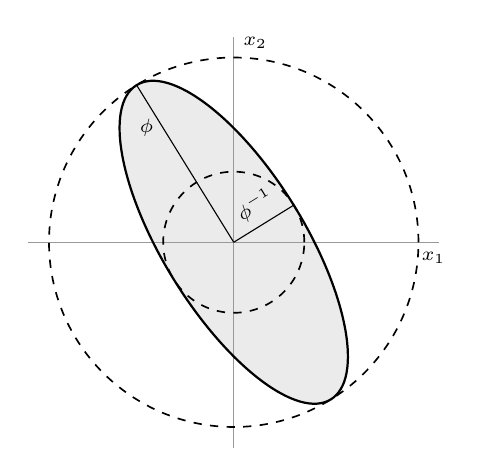
\begin{tikzpicture}[scale=1.45]
\fill[black!8, rotate=31.7175] (0,0) ellipse (0.618034 and 1.618034);
\draw[black!40, line width=0.4pt] (-1.8,0) -- (1.8,0);
\draw[black!40, line width=0.4pt] (0,-1.8) -- (0,1.8);
\draw[black, line width=0.8pt, rotate=31.7175] (0,0) ellipse (0.618034 and 1.618034);
\draw[black, dashed, line width=0.6pt] (0,0) circle (0.618034);
\draw[black, dashed, line width=0.6pt] (0,0) circle (1.618034);
\draw[line width=0.4pt, rotate=31.7175] (0,0) -- (0.618034,0);
\draw[line width=0.4pt, rotate=31.7175] (0,0) -- (0,1.618034);
\node[font=\scriptsize, rotate=31.7175] at (31.7175:0.33) [above] {$\phi^{-1}$};
\node[font=\scriptsize] at (121.7175:1.18) [left] {$\phi$};
\node[font=\scriptsize] at (1.75,0) [below] {$x_1$};
\node[font=\scriptsize] at (0,1.75) [right] {$x_2$};
\end{tikzpicture}}{The unit ball $\{x: x^{\mathsf T}Ax\le1\}$ of the norm $\|\cdot\|_A$ for the positive definite matrix $A$ with the rows $(2,1)$ and $(1,1)$ (shaded ellipse), and the Euclidean discs of radii $\phi^{-1}$ and $\phi$ (dashed), where $\phi$ is the golden ratio. The ellipse lies between the two discs and touches each in two points, on the eigenvectors of $A$; this is the inequality $\phi^{-1}\|x\|_2\le\|x\|_A\le\phi\|x\|_2$ with the best constants.\label{fig:norm-sandwich}}
\end{figure}

\begin{corollary}[Finite-dimensional normed spaces]
\label{cor:finite-dimensional}
Let $X$ be a finite-dimensional normed space with a basis $b_1,\ldots,b_n$.
\begin{enumerate}
\item A sequence $x^{(m)}=\sum_ja^{(m)}_jb_j$ converges to $x=\sum_ja_jb_j$ if and only if $a^{(m)}_j\to a_j$ for every $j$.
\item $X$ is complete, that is, a Banach space.
\item Every finite-dimensional subspace of a normed space is closed.
\item Every linear map from $X$ to a normed space $Y$ is bounded. Hence $\mathcal L(X,Y)$ consists of all linear maps from $X$ to $Y$.
\item A subset of $X$ is compact if and only if it is closed and bounded.
\item For every nonempty closed set $F\subseteq X$ and every $x\in X$ there is a nearest point of $F$ to $x$.
\end{enumerate}
\end{corollary}

\begin{proof}
By \cref{thm:norms-equivalent}, $\|\cdot\|$ is equivalent to the norm $|x|_\infty=\max_j|a_j|$ of the proof, and by \cref{prop:equivalent-norms} and \cref{prop:cauchy-basic}\,(iv) the two norms have the same convergent sequences, Cauchy sequences, closed sets, bounded sets and compact sets. (i) In the norm $|\cdot|_\infty$, convergence means convergence of the coefficients. (ii) The coordinate map identifies $(X,|\cdot|_\infty)$ isometrically with $(\mathbb F^n,\|\cdot\|_\infty)$, which is complete, as observed in \cref{sec:completeness-metric}. (iii) A finite-dimensional subspace $Y$ of a normed space is complete by (ii), applied to $Y$ with the restricted norm, and therefore closed by \cref{prop:closed-complete}. (iv) For a linear $T$ and $x=\sum_ja_jb_j$, $\|Tx\|\le\sum_j|a_j|\,\|Tb_j\|\le\bigl(\sum_j\|Tb_j\|\bigr)|x|_\infty\le C'\|x\|$ for a constant $C'$. (v) In $(X,|\cdot|_\infty)$, which is isometric to $(\mathbb F^n,\|\cdot\|_\infty)$, this is the Heine--Borel theorem. (vi) As for $\mathbb R^n$ after \cref{prop:compact-distance}: the set $F\cap\bar B(x,\|x-y_0\|)$ with $y_0\in F$ is nonempty, closed and bounded, hence compact by (v), and a nearest point of it to $x$ is a nearest point of $F$.
\end{proof}

Part (iv) extends \cref{prop:finite-dim-bounded} from the spaces $\mathbb F^n$ with the $p$-norms to all finite-dimensional normed spaces, as announced in \cref{sec:bounded-linear}, and it shows that the notation $\mathcal L(X,Y)$ of Volume~II, which there meant all linear maps, agrees with that of \cref{ch:metric-spaces} whenever $X$ is finite-dimensional. Part (iii) has a concrete meaning in approximation theory. The polynomials of degree at most $n$ form a subspace of dimension $n+1$ of $C[a,b]$, so they form a closed subspace for each of the norms $\|\cdot\|_\infty$, $\|\cdot\|_1$ and $\|\cdot\|_2$: a limit of polynomials of degree at most $n$ in any of these norms is a polynomial of degree at most $n$. The space of all polynomials, which is infinite-dimensional, is not closed: the Taylor polynomials $\sum_{k\le m}x^k/k!$ converge to $e^x$ in the supremum norm on $[0,1]$, with the error at most $e/(m+1)!$ by \vcref{1}{thm:taylor-lagrange}, and $e^x$ is not a polynomial, since no derivative of it vanishes identically.

The compactness of the unit sphere in finite dimensions also explains why the supremum in the definition of an operator norm is a maximum there, as \vcref{1}{sec:limits-rn} observed for $\|A\|_2$: if $X$ is finite-dimensional and $X\ne\{0\}$, the continuous function $x\mapsto\|Tx\|$ attains its maximum on the compact unit sphere $\{x: \|x\|=1\}$, which is $\|T\|$. In infinite dimensions the supremum need not be attained. The multiplier $M_a$ on $\ell^2$ with $a_k=1-1/k$ of \cref{sec:bounded-linear} has $\|M_a\|=\|a\|_\infty=1$, but $\|M_ax\|_2^2=\sum_k(1-1/k)^2|x_k|^2<\|x\|_2^2$ for every $x\ne0$.

\subsection{What Equivalence Means in Computation}

In $\mathbb F^n$ the theorem says that the choice of a norm does not affect which sequences converge, which sets are open, closed, bounded or compact, or which maps are continuous. Numerical analysis exploits this freedom constantly: to prove that an iteration converges, one may choose whatever norm makes the proof easiest, as \cref{thm:jacobi-contraction} did with $\|\cdot\|_\infty$ for matrices that are diagonally dominant by rows and with a weighted $1$-norm for those that are diagonally dominant by columns. The constants of equivalence, however, depend on the norms and on the dimension. On $\mathbb F^n$ the best constants between the $p$-norms are those of \cref{prop:p-norm-monotone}: $\|x\|_\infty\le\|x\|_2\le\|x\|_1\le\sqrt n\,\|x\|_2\le n\|x\|_\infty$, with equality for $\mathbf e_1$ in the first two and for $(1,\ldots,1)$ in the last two. For matrices, \vcref{2}{prop:norm-comparison} gives $\|A\|_\infty/\sqrt n\le\|A\|_2\le\sqrt m\,\|A\|_\infty$ for $A\in\mathbb F^{m\times n}$. A statement such as ``the error is below $10^{-8}$'' therefore means different things in different norms, and in dimension $10^6$ the difference between $\|\cdot\|_\infty$ and $\|\cdot\|_1$ is a factor of up to $10^6$. \Cref{sec:compact-computation} measures how large the factor typically is.

What does not depend on the norm is the rate at which an iteration converges, in the following sense.

\begin{proposition}[Rates of convergence do not depend on the norm]
\label{prop:rate-norm-independent}
Let $\|\cdot\|$ and $\|\cdot\|'$ be norms on a finite-dimensional space $X$, with $c\|x\|\le\|x\|'\le C\|x\|$, and let $(e_k)$ be a sequence in $X$.
\begin{enumerate}
\item If $\|e_k\|\le Mq^k$ for all $k$, then $\|e_k\|'\le CMq^k$ for all $k$.
\item $\limsup_{k\to\infty}\|e_k\|^{1/k}=\limsup_{k\to\infty}(\|e_k\|')^{1/k}$: the \term{asymptotic rate} of the sequence is the same in all norms.
\end{enumerate}
\end{proposition}

\begin{proof}
(i) is immediate. (ii) Write $u_k\coloneqq\|e_k\|^{1/k}$ and $u'_k\coloneqq(\|e_k\|')^{1/k}$. Then $c^{1/k}u_k\le u'_k\le C^{1/k}u_k$, and $c^{1/k}\to1$ and $C^{1/k}\to1$ (\vcref{1}{thm:standard-limits}). So a subsequence of $(u_k)$ converges to some $\lambda\in[0,\infty]$ if and only if the corresponding subsequence of $(u'_k)$ does, by the squeeze theorem, and by \cref{thm:limsup-properties}\,(ii) the largest subsequential limits of the two sequences agree.
\end{proof}

For the errors $e_k=G^k e_0$ of a linear iteration with a matrix $G$, the asymptotic rate is at most $\lim_k\|G^k\|^{1/k}=\rho(G)$, the spectral radius, by Gelfand's formula (\vcref{2}{thm:gelfand}); the proposition explains why this limit is the same for every matrix norm. A change of norm changes the number of steps needed to reach a tolerance by a bounded amount: if $\|e_k\|$ decreases exactly like $q^k$, the tolerance $\tau$ is reached in the norm $\|\cdot\|'$ at most $\ln(C/c)/\ln(1/q)$ steps earlier or later than in the norm $\|\cdot\|$, up to rounding of the step numbers. \Cref{sec:compact-computation} observes this for the Jacobi iteration.

\subsection{Riesz's Lemma}

In infinite dimensions the closed unit ball is not compact, as \cref{prop:l2-ball-not-compact} showed for $\ell^p$. The note in \vcref{2}{sec:spectral-theorem} used the same fact to explain why the spectral theorem fails for self-adjoint operators in general. The following lemma of F.~Riesz shows that this happens in every infinite-dimensional normed space. It replaces orthogonality, which is not available in a general normed space, by an approximate substitute.

\begin{lemma}[Riesz's lemma]
\label{lem:riesz}
Let $Y$ be a closed subspace of a normed space $X$ with $Y\ne X$, and let $0<\theta<1$. There is $x\in X$ with $\|x\|=1$ and $\operatorname{dist}(x,Y)\ge\theta$. If $Y$ is finite-dimensional, there is such an $x$ with $\operatorname{dist}(x,Y)=1$.
\end{lemma}

\begin{proof}
Choose $x_0\in X\setminus Y$. Since $Y$ is closed, $d\coloneqq\operatorname{dist}(x_0,Y)>0$ by \cref{prop:closure}\,(iv). As $d/\theta>d$, there is $y_0\in Y$ with $\|x_0-y_0\|\le d/\theta$. Let $x\coloneqq(x_0-y_0)/\|x_0-y_0\|$, so that $\|x\|=1$. For $y\in Y$,
\[
\|x-y\|=\frac{\bigl\|x_0-\bigl(y_0+\|x_0-y_0\|\,y\bigr)\bigr\|}{\|x_0-y_0\|}\ge\frac d{d/\theta}=\theta,
\]
because $y_0+\|x_0-y_0\|\,y$ lies in $Y$, so that the numerator is at least $d$. If $Y$ is finite-dimensional, a nearest point $y_0$ of $Y$ to $x_0$ exists by \cref{cor:finite-dimensional}\,(vi), applied in the finite-dimensional space $\operatorname{span}(Y\cup\{x_0\})$; then $\|x_0-y_0\|=d$, and the same computation gives $\|x-y\|\ge1$ for all $y\in Y$, while $y=0$ gives $\|x-0\|=1$.
\end{proof}

In an inner product space, a unit vector orthogonal to $Y$ has distance exactly $1$ from $Y$, by Pythagoras, and the lemma would be trivial if such vectors existed. In a general normed space there is no orthogonality, and the lemma produces a unit vector that is almost as far from $Y$ as an orthogonal one would be.

\begin{theorem}[Riesz]
\label{thm:riesz-compact}
For a normed space $X$ the following are equivalent:
\begin{enumerate}
\item $X$ is finite-dimensional;
\item the closed unit ball $\bar B(0,1)$ of $X$ is compact;
\item every bounded sequence in $X$ has a convergent subsequence.
\end{enumerate}
\end{theorem}

\begin{proof}
(i)$\Rightarrow$(iii) Let $(x_n)$ be bounded. The closed ball $\bar B(0,R)$ that contains it is closed and bounded, hence compact by \cref{cor:finite-dimensional}\,(v), and \cref{thm:compact-equivalences} gives a convergent subsequence. (iii)$\Rightarrow$(ii) Every sequence in $\bar B(0,1)$ is bounded and has a convergent subsequence, whose limit lies in the closed ball; so the ball is sequentially compact, hence compact. (ii)$\Rightarrow$(i) Suppose that $X$ is infinite-dimensional. We construct unit vectors $x_1,x_2,\ldots$ with $\|x_m-x_n\|\ge1$ for $m\ne n$. Choose any unit vector $x_1$. If $x_1,\ldots,x_n$ have been chosen, their span $Y_n$ is finite-dimensional, hence closed by \cref{cor:finite-dimensional}\,(iii), and different from $X$. By \cref{lem:riesz}, there is a unit vector $x_{n+1}$ with $\operatorname{dist}(x_{n+1},Y_n)=1$, so $\|x_{n+1}-x_m\|\ge1$ for $m\le n$. The sequence $(x_n)$ lies in the closed unit ball and has no Cauchy subsequence, hence no convergent one, so the ball is not compact.
\end{proof}

The theorem turns the remark of the note in \vcref{2}{sec:spectral-theorem}, that ``the unit sphere is no longer compact'', into a statement about every infinite-dimensional normed space. In $\ell^p$ the unit sequences are an explicit sequence of the kind constructed in the proof. In $C[0,1]$ with the supremum norm, the monomials $x^n$ are another: they lie in the unit ball, and no subsequence converges, since by \cref{sec:open-closed} a uniform limit would have to agree with the discontinuous pointwise limit. The theorem also shows that in an infinite-dimensional normed space no closed ball $\bar B(a,r)$ is compact, because it is a translated and scaled copy of the unit ball, and consequently no compact set has an interior point. Compact sets in infinite dimensions are thin, like the Hilbert cube of \cref{prop:hilbert-cube}.

\subsection{Best Approximation}

Approximating a complicated object by a simple one is the basic operation of numerical analysis: a function by a polynomial, a vector by an element of a subspace, a matrix by one of low rank. When the simple objects form a finite-dimensional subspace, a best approximation always exists.

\begin{theorem}[Existence of best approximations]
\label{thm:best-approximation-normed}
Let $Y$ be a finite-dimensional subspace of a normed space $X$. For every $x\in X$ there is $y^*\in Y$ with
\[
\|x-y^*\|=\operatorname{dist}(x,Y)=\min_{y\in Y}\|x-y\| .
\]
The set of all such $y^*$ is compact and convex.
\end{theorem}

\begin{proof}
The subspace $Y$ is closed by \cref{cor:finite-dimensional}\,(iii). Apply \cref{cor:finite-dimensional}\,(vi) in the finite-dimensional space $\operatorname{span}(Y\cup\{x\})$, in which $Y$ is a nonempty closed set. The set $M$ of best approximations is $Y\cap\bar B(x,d)$ with $d\coloneqq\operatorname{dist}(x,Y)$, which is closed and bounded in $Y$, hence compact by \cref{cor:finite-dimensional}\,(v); and if $y_1,y_2\in M$ and $0\le t\le1$, then $\|x-(ty_1+(1-t)y_2)\|\le t\|x-y_1\|+(1-t)\|x-y_2\|=d$, so $ty_1+(1-t)y_2\in M$.
\end{proof}

In an inner product space the best approximation is unique and is the orthogonal projection, \vcref{2}{thm:best-approximation}. In other norms it need not be unique. In $\mathbb R^2$ with $\|\cdot\|_1$, the distance of $x=(1,0)$ from the line $Y=\{t(1,1): t\in\mathbb R\}$ is $\min_t(|1-t|+|t|)=1$, attained by every $t\in[0,1]$, a whole segment of best approximations, as the theorem allows. For the supremum norm on $C[a,b]$ and the polynomials of degree at most $n$, the theorem gives the existence of a best uniform approximation of every continuous function, which is the starting point of Chebyshev's theory of minimax approximation; there the best approximation is unique, for a reason particular to polynomials, and Volume~XI develops this theory and the algorithms that compute it. If $Y$ is infinite-dimensional, even closed, a best approximation need not exist, as the example at the end of \cref{sec:compact-continuous} indicates for closed sets; in Hilbert spaces it always exists for closed subspaces, by the projection theorem of Chapter~22.

\section{Connectedness}
\label{sec:connectedness}

\subsection{Connected Spaces}

\begin{definition}[Connected space]
\label{def:connected}
A \term{separation} of a metric space $X$ is a pair of disjoint nonempty open sets $U$ and $V$ with $X=U\cup V$. The space $X$ is \term{connected} if it has no separation, and \term{disconnected} otherwise. A subset of $X$ is connected if it is connected as a metric space with the restricted metric.
\end{definition}

The empty set and every one-point set are connected. The subspace $\mathbb Q$ of $\mathbb R$ is disconnected: \cref{sec:open-closed} found the separation of $\mathbb Q$ into the open sets $\{q: q^2<2\}$ and $\{q: q^2>2\}$, which is the splitting that \cref{prop:ivt-completeness} associated with the failure of completeness. The set $[0,1]\cup[2,3]$ is disconnected, both intervals being open in the subspace, and so is every set with the discrete metric that has more than one point.

\begin{proposition}[Descriptions of connectedness]
\label{prop:connected-characterisations}
For a metric space $X$ the following are equivalent:
\begin{enumerate}
\item $X$ is connected;
\item the only subsets of $X$ that are both open and closed are $\emptyset$ and $X$;
\item every continuous function from $X$ to the two-point space $\{0,1\}$ with the discrete metric is constant.
\end{enumerate}
A subset $S$ of $X$ is disconnected if and only if there are open sets $U$ and $V$ of $X$ with $S\subseteq U\cup V$, $S\cap U\cap V=\emptyset$, and $S\cap U\ne\emptyset\ne S\cap V$.
\end{proposition}

\begin{proof}
If $U,V$ is a separation, $U$ is open, and closed since its complement $V$ is open, and it is neither $\emptyset$ nor $X$; conversely, a set $U$ that is open and closed and different from $\emptyset$ and $X$ forms a separation with $X\setminus U$. So (i) and (ii) are equivalent. A continuous $f\colon X\to\{0,1\}$ gives the open and closed set $f^{-1}(\{0\})$, since $\{0\}$ is open and closed in $\{0,1\}$; conversely, an open and closed set $U$ gives the continuous indicator function $\mathbf 1_U$, whose preimages of all subsets of $\{0,1\}$ are among $\emptyset$, $U$, $X\setminus U$ and $X$. So (ii) and (iii) are equivalent. The statement about subsets is the definition, with the open sets of $S$ written as $U\cap S$ and $V\cap S$ by \cref{prop:relative-open}.
\end{proof}

Description (iii) is the most convenient in proofs, as the following results show.

\begin{theorem}[Connected subsets of the line]
\label{thm:connected-real}
A subset of $\mathbb R$ is connected if and only if it is an interval.
\end{theorem}

\begin{proof}
Let $S\subseteq\mathbb R$ be connected, and let $x,y\in S$ and $x<z<y$. If $z\notin S$, the open sets $(-\infty,z)$ and $(z,\infty)$ satisfy the condition of \cref{prop:connected-characterisations} for $S$, which is impossible; so $z\in S$, and $S$ is an interval by \vcref{1}{prop:intervals}.

Conversely, let $I$ be an interval and $f\colon I\to\{0,1\}$ continuous, and suppose $f$ is not constant: $f(a)\ne f(b)$ for some $a<b$ in $I$. Replacing $f$ by $1-f$ if necessary, we may assume $f(a)=0$. Continuity into the discrete space $\{0,1\}$ means that every point $x$ of $I$ has a $\delta>0$ such that $f$ is constant on $(x-\delta,x+\delta)\cap I$. Let
\[
s\coloneqq\sup\{x\in[a,b]: f=0\text{ on }[a,x]\},
\]
which lies in $[a,b]$, and choose $\delta$ for the point $s$. There are points $x\in(s-\delta,s]$ with $f=0$ on $[a,x]$, so $f(s)=0$, the value of $f$ near $s$, and $f=0$ on $[a,s]$ as well as on $[s,s+\delta)\cap[a,b]$. If $s<b$, this contradicts the definition of $s$; so $s=b$ and $f(b)=0$, a contradiction.
\end{proof}

The second half of the proof is the supremum argument of \cref{thm:interval-compact} once more, and it uses the completeness of $\mathbb R$ in the same way. \Cref{prop:ivt-completeness} showed that, among ordered fields, the complete ones are exactly those in which the closed intervals are connected in this sense.

\begin{theorem}[Continuous images of connected spaces]
\label{thm:connected-image}
Let $f\colon X\to Y$ be continuous. If $X$ is connected, so is $f(X)$.
\end{theorem}

\begin{proof}
If $g\colon f(X)\to\{0,1\}$ is continuous, then $g\circ f\colon X\to\{0,1\}$ is continuous and therefore constant, so $g$ is constant on $f(X)$.
\end{proof}

\begin{corollary}[Intermediate value theorem]
\label{cor:ivt-general}
Let $X$ be connected and $f\colon X\to\mathbb R$ continuous. If $a,b\in X$ and $y$ lies between $f(a)$ and $f(b)$, then $y=f(c)$ for some $c\in X$.
\end{corollary}

\begin{proof}
$f(X)$ is a connected subset of $\mathbb R$, hence an interval by \cref{thm:connected-real}, and it contains $f(a)$ and $f(b)$.
\end{proof}

For $X=[a,b]$ and for an arbitrary interval this is \vcref{1}{cor:ivt} and \vcref{1}{cor:interval-image}, and the promise of \cref{prop:ivt-completeness} to develop connectedness in general is kept. The corollary applies far beyond intervals. If $f$ is a continuous function on the unit circle $S^1\subseteq\mathbb R^2$, for instance the temperature along the equator, then $g(x)\coloneqq f(x)-f(-x)$ is continuous with $g(-x)=-g(x)$; it takes values of both signs, or vanishes, and since $S^1$ is connected, being the image of $[0,2\pi]$ under $t\mapsto(\cos t,\sin t)$, it has a zero. There are always two opposite points of the circle with the same value of $f$.

\subsection{Unions, Closures and Components}

\begin{proposition}[Building connected sets]
\label{prop:connected-unions}
Let $X$ and $Y$ be metric spaces.
\begin{enumerate}
\item If $(C_i)_{i\in I}$ is a family of connected subsets of $X$ and $C_0$ is a connected subset that meets every $C_i$, then $C_0\cup\bigcup_iC_i$ is connected. In particular, connected sets with a common point have a connected union.
\item If $C\subseteq X$ is connected and $C\subseteq S\subseteq\overline C$, then $S$ is connected; in particular $\overline C$ is connected.
\item If $X$ and $Y$ are connected, so is $X\times Y$ with the product metric.
\end{enumerate}
\end{proposition}

\begin{proof}
(i) Let $f$ be a continuous function from the union to $\{0,1\}$. It is constant on $C_0$, with a value $v$, and constant on every $C_i$, with the value $v$ because $C_i$ meets $C_0$. (ii) Let $f\colon S\to\{0,1\}$ be continuous; it is constant on $C$, with a value $v$. Every $s\in S$ is the limit of a sequence $(c_n)$ in $C$, by \cref{prop:closure-sequences}, so $f(s)=\lim f(c_n)=v$. (iii) Fix $y_0\in Y$. For each $x\in X$ the sets $X\times\{y_0\}$ and $\{x\}\times Y$ are connected, as images of $X$ and $Y$ under continuous maps, and they meet in $(x,y_0)$; so their union $T_x$ is connected by (i). The sets $T_x$ all contain the connected set $X\times\{y_0\}$, and their union is $X\times Y$, which is therefore connected by (i).
\end{proof}

By (iii) and induction, $\mathbb R^n$ and every box $I_1\times\cdots\times I_n$ of intervals are connected, with the product metric, and hence with every norm, since connectedness depends only on the open sets.

\begin{definition}[Component]
\label{def:component}
Let $X$ be a metric space and $x\in X$. The \term{component} of $x$ in $X$ is the union of all connected subsets of $X$ that contain $x$.
\end{definition}

\begin{proposition}[Components]
\label{prop:components}
The component $C(x)$ of $x$ is connected, it contains every connected subset of $X$ that contains $x$, and it is closed. Two components are equal or disjoint, so that the components form a partition of $X$; every connected subset of $X$ lies in exactly one component, if it is nonempty.
\end{proposition}

\begin{proof}
$C(x)$ is a union of connected sets with the common point $x$, hence connected by \cref{prop:connected-unions}\,(i), and it contains every connected set that contains $x$ by definition. Its closure is connected by \cref{prop:connected-unions}\,(ii) and contains $x$, so it lies in $C(x)$, and $C(x)$ is closed. If $C(x)$ and $C(y)$ have a point in common, their union is connected and contains $x$ and $y$, so it lies in $C(x)$ and in $C(y)$, and the two components are equal. A nonempty connected set $S$ with a point $x$ lies in $C(x)$.
\end{proof}

A space is connected if and only if it has exactly one component, or is empty. The components of $[0,1]\cup[2,3]$ are the two intervals, and those of $\mathbb Q$ are its one-point sets, since a connected subset of $\mathbb Q$ with two points $p<q$ would be an interval of $\mathbb R$, by \cref{thm:connected-real}, containing the irrational numbers between $p$ and $q$. For open subsets of $\mathbb R$ the components have a simple description.

\begin{theorem}[Open subsets of the line]
\label{thm:open-sets-real}
Every open set $U\subseteq\mathbb R$ is the union of countably many disjoint open intervals, namely its components, and there is no other way of writing $U$ as a union of disjoint open intervals.
\end{theorem}

\begin{proof}
A component $C$ of $U$ is an interval by \cref{thm:connected-real}. It is open: if $x\in C$ and $(x-r,x+r)\subseteq U$, this interval is connected and meets $C$, so it lies in $C$ by \cref{prop:components}. The components are disjoint, cover $U$, and each contains a rational number. Let $q_0,q_1,\ldots$ be an enumeration of $\mathbb Q$ (\vcref{1}{thm:q-countable}), and assign to each component the smallest $k$ with $q_k\in C$; this is an injection of the set of components into $\mathbb N$, so there are countably many of them. If $U=\bigcup_jI_j$ with disjoint open intervals $I_j$, each $I_j$ is connected and lies in a component $C$; and $C$ is the union of the disjoint open sets $C\cap I_j$, so by connectedness only one of them is nonempty, and $C=I_j$.
\end{proof}

The complement of the Cantor set in $(0,1)$ is an example: it is open, and its components are the countably many removed middle thirds $(1/3,2/3)$, $(1/9,2/9)$, $(7/9,8/9)$, and so on. The same argument shows that in a normed space the components of an open set are open, since balls are convex and therefore connected (\cref{prop:path-connected} below), and that in a separable normed space, such as $\mathbb R^n$, an open set has at most countably many components.

\subsection{Path-Connected Spaces}

\begin{definition}[Path, path-connected space]
\label{def:path-connected}
A \term{path} in a metric space $X$ from $x$ to $y$ is a continuous map $\gamma\colon[0,1]\to X$ with $\gamma(0)=x$ and $\gamma(1)=y$. The space $X$ is \term{path-connected} if any two of its points are joined by a path in $X$.
\end{definition}

Paths can be reversed, $t\mapsto\gamma(1-t)$, and joined: if $\gamma$ runs from $x$ to $y$ and $\eta$ from $y$ to $z$, the map that equals $\gamma(2t)$ for $t\le1/2$ and $\eta(2t-1)$ for $t\ge1/2$ is continuous, since its two pieces agree at $t=1/2$, and runs from $x$ to $z$.

\begin{proposition}[Path-connected spaces]
\label{prop:path-connected}
\leavevmode
\begin{enumerate}
\item Every path-connected space is connected.
\item Every convex subset of a normed space is path-connected, in particular every ball and every subspace.
\item The continuous image of a path-connected space is path-connected.
\item In a normed space $X$ of dimension at least $2$, the set $X\setminus\{0\}$ and the unit sphere $\{x: \|x\|=1\}$ are path-connected.
\end{enumerate}
\end{proposition}

\begin{proof}
(i) Let $x\in X$. For every $y\in X$, a path from $x$ to $y$ has a connected image, by \cref{thm:connected-image,thm:connected-real}, which contains $x$ and $y$; so $y$ lies in the component $C(x)$, and $X=C(x)$ is connected. (ii) For $x$ and $y$ in a convex set, $t\mapsto(1-t)x+ty$ is a path in the set, continuous by \cref{prop:distance-lipschitz}. (iii) If $\gamma$ joins $x$ and $y$, then $f\circ\gamma$ joins $f(x)$ and $f(y)$. (iv) Let $x,y\ne0$. If $0$ does not lie on the segment from $x$ to $y$, the segment is a path in $X\setminus\{0\}$. Otherwise $y=-sx$ with $s>0$; choose $z$ outside the one-dimensional space spanned by $x$, which exists since $\dim X\ge2$; the segments from $x$ to $z$ and from $z$ to $y$ do not pass through $0$, because $0=(1-t)x+tz$ with $0<t\le1$ would put $z$ in the span of $x$, and similarly for $y$. The sphere is the image of $X\setminus\{0\}$ under the continuous map $x\mapsto x/\|x\|$.
\end{proof}

As for components, the \term{path component} of a point $x$ is the set of all points that can be joined to $x$ by a path. Since paths can be reversed and joined, the path components partition the space, and each lies in a component, by \cref{prop:path-connected}\,(i). The open set $\mathbb R^2\setminus\{(x,0): x\in\mathbb R\}$ has the two path components $\{y>0\}$ and $\{y<0\}$, which are also its components; \cref{sec:matrix-paths} finds the path components of the invertible matrices. In general a component may consist of several path components.

The converse of (i) fails, and the standard counterexample is drawn in \cref{fig:sine-curve}.

\begin{figure}
\sdfloat{%
\begin{tikzpicture}
\begin{axis}[sdplot, width=0.62\textwidth, height=0.34\textwidth, xmin=-0.03, xmax=1.02, ymin=-1.15, ymax=1.15,
  xtick={0,0.5,1}, ytick={-1,0,1}, xlabel={$x$}]
\addplot[black, line width=0.35pt] coordinates {(1.00000,0.8415) (0.90909,0.8912) (0.83333,0.9320) (0.76923,0.9636) (0.71429,0.9854) (0.66667,0.9975) (0.62500,0.9996) (0.58824,0.9917) (0.55556,0.9738) (0.52632,0.9463) (0.50000,0.9093) (0.47619,0.8632) (0.45455,0.8085) (0.43478,0.7457) (0.41667,0.6755) (0.40000,0.5985) (0.38462,0.5155) (0.37037,0.4274) (0.35714,0.3350) (0.34483,0.2392) (0.33333,0.1411) (0.32258,0.0416) (0.31250,-0.0584) (0.30303,-0.1577) (0.29412,-0.2555) (0.28571,-0.3508) (0.27778,-0.4425) (0.27027,-0.5298) (0.26316,-0.6119) (0.25641,-0.6878) (0.25000,-0.7568) (0.24390,-0.8183) (0.23810,-0.8716) (0.23256,-0.9162) (0.22727,-0.9516) (0.22222,-0.9775) (0.21739,-0.9937) (0.21277,-0.9999) (0.20833,-0.9962) (0.20408,-0.9825) (0.20000,-0.9589) (0.19608,-0.9258) (0.19231,-0.8835) (0.18868,-0.8323) (0.18519,-0.7728) (0.18182,-0.7055) (0.17857,-0.6313) (0.17544,-0.5507) (0.17241,-0.4646) (0.16949,-0.3739) (0.16667,-0.2794) (0.16393,-0.1822) (0.16129,-0.0831) (0.15873,0.0168) (0.15625,0.1165) (0.15385,0.2151) (0.15152,0.3115) (0.14925,0.4048) (0.14706,0.4941) (0.14493,0.5784) (0.14286,0.6570) (0.14085,0.7290) (0.13889,0.7937) (0.13699,0.8504) (0.13514,0.8987) (0.13333,0.9380) (0.13158,0.9679) (0.12987,0.9882) (0.12821,0.9985) (0.12658,0.9989) (0.12500,0.9894) (0.12346,0.9699) (0.12195,0.9407) (0.12048,0.9022) (0.11905,0.8546) (0.11765,0.7985) (0.11628,0.7344) (0.11494,0.6630) (0.11364,0.5849) (0.11236,0.5010) (0.11111,0.4121) (0.10989,0.3191) (0.10870,0.2229) (0.10753,0.1245) (0.10638,0.0248) (0.10526,-0.0752) (0.10417,-0.1743) (0.10309,-0.2718) (0.10204,-0.3665) (0.10101,-0.4575) (0.10000,-0.5440) (0.09901,-0.6251) (0.09804,-0.6999) (0.09709,-0.7677) (0.09615,-0.8278) (0.09524,-0.8797) (0.09434,-0.9228) (0.09346,-0.9566) (0.09259,-0.9809) (0.09174,-0.9954) (0.09091,-1.0000) (0.09009,-0.9946) (0.08929,-0.9792) (0.08850,-0.9540) (0.08772,-0.9193) (0.08696,-0.8755) (0.08621,-0.8228) (0.08547,-0.7620) (0.08475,-0.6935) (0.08403,-0.6181) (0.08333,-0.5366) (0.08264,-0.4496) (0.08197,-0.3582) (0.08130,-0.2632) (0.08065,-0.1656) (0.08000,-0.0663) (0.07937,0.0336) (0.07874,0.1332) (0.07813,0.2315) (0.07752,0.3275) (0.07692,0.4202) (0.07634,0.5087) (0.07576,0.5921) (0.07519,0.6696) (0.07463,0.7404) (0.07407,0.8038) (0.07353,0.8592) (0.07299,0.9060) (0.07246,0.9437) (0.07194,0.9720) (0.07143,0.9906) (0.07092,0.9993) (0.07042,0.9980) (0.06993,0.9868) (0.06944,0.9657) (0.06897,0.9349) (0.06849,0.8948) (0.06803,0.8457) (0.06757,0.7883) (0.06711,0.7229) (0.06667,0.6503) (0.06623,0.5712) (0.06579,0.4864) (0.06536,0.3967) (0.06494,0.3031) (0.06452,0.2065) (0.06410,0.1078) (0.06369,0.0080) (0.06329,-0.0919) (0.06289,-0.1909) (0.06250,-0.2879) (0.06211,-0.3821) (0.06173,-0.4724) (0.06135,-0.5581) (0.06098,-0.6381) (0.06061,-0.7118) (0.06024,-0.7784) (0.05988,-0.8371) (0.05952,-0.8876) (0.05917,-0.9291) (0.05882,-0.9614) (0.05848,-0.9841) (0.05814,-0.9969) (0.05780,-0.9998) (0.05747,-0.9927) (0.05714,-0.9756) (0.05682,-0.9488) (0.05650,-0.9126) (0.05618,-0.8672) (0.05587,-0.8132) (0.05556,-0.7510) (0.05525,-0.6813) (0.05495,-0.6048) (0.05464,-0.5223) (0.05435,-0.4346) (0.05405,-0.3425) (0.05376,-0.2470) (0.05348,-0.1490) (0.05319,-0.0495) (0.05291,0.0504) (0.05263,0.1499) (0.05236,0.2478) (0.05208,0.3433) (0.05181,0.4354) (0.05155,0.5231) (0.05128,0.6055) (0.05102,0.6820) (0.05076,0.7516) (0.05051,0.8137) (0.05025,0.8676) (0.05000,0.9129) (0.04975,0.9491) (0.04950,0.9758) (0.04926,0.9928) (0.04902,0.9998) (0.04878,0.9968) (0.04854,0.9839) (0.04831,0.9612) (0.04808,0.9288) (0.04785,0.8872) (0.04762,0.8367) (0.04739,0.7778) (0.04717,0.7112) (0.04695,0.6374) (0.04673,0.5573) (0.04651,0.4716) (0.04630,0.3813) (0.04608,0.2871) (0.04587,0.1900) (0.04566,0.0910) (0.04545,-0.0089) (0.04525,-0.1086) (0.04505,-0.2073) (0.04484,-0.3040) (0.04464,-0.3976) (0.04444,-0.4872) (0.04425,-0.5719) (0.04405,-0.6510) (0.04386,-0.7235) (0.04367,-0.7888) (0.04348,-0.8462) (0.04329,-0.8952) (0.04310,-0.9352) (0.04292,-0.9659) (0.04274,-0.9869) (0.04255,-0.9981) (0.04237,-0.9993) (0.04219,-0.9905) (0.04202,-0.9718) (0.04184,-0.9434) (0.04167,-0.9056) (0.04149,-0.8587) (0.04132,-0.8033) (0.04115,-0.7398) (0.04098,-0.6689) (0.04082,-0.5914) (0.04065,-0.5079) (0.04049,-0.4194) (0.04032,-0.3266) (0.04016,-0.2306) (0.04000,-0.1324) (0.03984,-0.0327) (0.03968,0.0672) (0.03953,0.1665) (0.03937,0.2641) (0.03922,0.3591) (0.03906,0.4504) (0.03891,0.5373) (0.03876,0.6188) (0.03861,0.6942) (0.03846,0.7626) (0.03831,0.8233) (0.03817,0.8759) (0.03802,0.9197) (0.03788,0.9543) (0.03774,0.9794) (0.03759,0.9946) (0.03745,1.0000) (0.03731,0.9954) (0.03717,0.9808) (0.03704,0.9564) (0.03690,0.9224) (0.03676,0.8793) (0.03663,0.8273) (0.03650,0.7671) (0.03636,0.6992) (0.03623,0.6244) (0.03610,0.5433) (0.03597,0.4567) (0.03584,0.3657) (0.03571,0.2709) (0.03559,0.1735) (0.03546,0.0743) (0.03534,-0.0257) (0.03521,-0.1253) (0.03509,-0.2238) (0.03497,-0.3199) (0.03484,-0.4129) (0.03472,-0.5018) (0.03460,-0.5856) (0.03448,-0.6636) (0.03436,-0.7350) (0.03425,-0.7990) (0.03413,-0.8551) (0.03401,-0.9026) (0.03390,-0.9410) (0.03378,-0.9701) (0.03367,-0.9895) (0.03356,-0.9990) (0.03344,-0.9985) (0.03333,-0.9880) (0.03322,-0.9677) (0.03311,-0.9377) (0.03300,-0.8983) (0.03289,-0.8500) (0.03279,-0.7931) (0.03268,-0.7284) (0.03257,-0.6563) (0.03247,-0.5777) (0.03236,-0.4933) (0.03226,-0.4040) (0.03215,-0.3107) (0.03205,-0.2143) (0.03195,-0.1157) (0.03185,-0.0159) (0.03175,0.0840) (0.03165,0.1830) (0.03155,0.2803) (0.03145,0.3747) (0.03135,0.4654) (0.03125,0.5514) (0.03115,0.6320) (0.03106,0.7062) (0.03096,0.7733) (0.03086,0.8328) (0.03077,0.8839) (0.03067,0.9262) (0.03058,0.9592) (0.03049,0.9826) (0.03040,0.9962) (0.03030,0.9999) (0.03021,0.9936) (0.03012,0.9773) (0.03003,0.9513) (0.02994,0.9158) (0.02985,0.8711) (0.02976,0.8178) (0.02967,0.7562) (0.02959,0.6871) (0.02950,0.6112) (0.02941,0.5291) (0.02933,0.4417) (0.02924,0.3500) (0.02915,0.2547) (0.02907,0.1569) (0.02899,0.0575) (0.02890,-0.0425) (0.02882,-0.1420) (0.02874,-0.2401) (0.02865,-0.3358) (0.02857,-0.4282) (0.02849,-0.5163) (0.02841,-0.5992) (0.02833,-0.6761) (0.02825,-0.7463) (0.02817,-0.8090) (0.02809,-0.8637) (0.02801,-0.9097) (0.02793,-0.9466) (0.02786,-0.9740) (0.02778,-0.9918) (0.02770,-0.9996) (0.02762,-0.9974) (0.02755,-0.9853) (0.02747,-0.9633) (0.02740,-0.9317) (0.02732,-0.8908) (0.02725,-0.8410) (0.02717,-0.7828) (0.02710,-0.7167) (0.02703,-0.6435) (0.02695,-0.5639) (0.02688,-0.4786) (0.02681,-0.3886) (0.02674,-0.2947) (0.02667,-0.1978) (0.02660,-0.0989) (0.02653,0.0009) (0.02646,0.1007) (0.02639,0.1995) (0.02632,0.2964) (0.02625,0.3902) (0.02618,0.4802) (0.02611,0.5654) (0.02604,0.6449) (0.02597,0.7180) (0.02591,0.7839) (0.02584,0.8420) (0.02577,0.8916) (0.02571,0.9324) (0.02564,0.9638) (0.02558,0.9856) (0.02551,0.9976) (0.02545,0.9995) (0.02538,0.9915) (0.02532,0.9736) (0.02525,0.9460) (0.02519,0.9089) (0.02513,0.8628) (0.02506,0.8080) (0.02500,0.7451) (0.02491,0.6371) (0.02481,0.5147) (0.02472,0.3808) (0.02463,0.2384) (0.02454,0.0906) (0.02445,-0.0593) (0.02436,-0.2078) (0.02427,-0.3516) (0.02418,-0.4876) (0.02410,-0.6126) (0.02401,-0.7238) (0.02392,-0.8188) (0.02384,-0.8954) (0.02375,-0.9519) (0.02367,-0.9870) (0.02358,-0.9999) (0.02350,-0.9904) (0.02342,-0.9587) (0.02334,-0.9054) (0.02326,-0.8318) (0.02317,-0.7395) (0.02309,-0.6306) (0.02301,-0.5075) (0.02294,-0.3731) (0.02286,-0.2302) (0.02278,-0.0822) (0.02270,0.0677) (0.02262,0.2160) (0.02255,0.3595) (0.02247,0.4949) (0.02240,0.6192) (0.02232,0.7296) (0.02225,0.8236) (0.02217,0.8991) (0.02210,0.9544) (0.02203,0.9883) (0.02195,1.0000) (0.02188,0.9892) (0.02181,0.9562) (0.02174,0.9018) (0.02167,0.8271) (0.02160,0.7338) (0.02153,0.6240) (0.02146,0.5003) (0.02139,0.3652) (0.02132,0.2220) (0.02125,0.0738) (0.02119,-0.0760) (0.02112,-0.2242) (0.02105,-0.3673) (0.02099,-0.5022) (0.02092,-0.6258) (0.02086,-0.7353) (0.02079,-0.8283) (0.02073,-0.9027) (0.02066,-0.9569) (0.02060,-0.9896) (0.02053,-1.0000) (0.02047,-0.9880) (0.02041,-0.9538) (0.02035,-0.8981) (0.02028,-0.8223) (0.02022,-0.7281) (0.02016,-0.6174) (0.02010,-0.4930) (0.02004,-0.3574) (0.01998,-0.2138) (0.01992,-0.0654) (0.01986,0.0844) (0.01980,0.2324) (0.01974,0.3751) (0.01969,0.5094) (0.01963,0.6323) (0.01957,0.7410) (0.01951,0.8330) (0.01946,0.9063) (0.01940,0.9593) (0.01934,0.9907) (0.01929,0.9999) (0.01923,0.9866) (0.01918,0.9512) (0.01912,0.8944) (0.01907,0.8175) (0.01901,0.7223) (0.01896,0.6108) (0.01890,0.4856) (0.01885,0.3495) (0.01880,0.2056) (0.01874,0.0570) (0.01869,-0.0928) (0.01864,-0.2405) (0.01859,-0.3829) (0.01854,-0.5166) (0.01848,-0.6388) (0.01843,-0.7466) (0.01838,-0.8376) (0.01833,-0.9099) (0.01828,-0.9616) (0.01823,-0.9918) (0.01818,-0.9998) (0.01813,-0.9852) (0.01808,-0.9486) (0.01803,-0.8906) (0.01799,-0.8126) (0.01794,-0.7164) (0.01789,-0.6041) (0.01784,-0.4783) (0.01779,-0.3416) (0.01775,-0.1974) (0.01770,-0.0486) (0.01765,0.1012) (0.01761,0.2487) (0.01756,0.3906) (0.01751,0.5238) (0.01747,0.6452) (0.01742,0.7522) (0.01738,0.8422) (0.01733,0.9133) (0.01729,0.9639) (0.01724,0.9929) (0.01720,0.9995) (0.01715,0.9837) (0.01711,0.9459) (0.01706,0.8867) (0.01702,0.8077) (0.01698,0.7105) (0.01693,0.5974) (0.01689,0.4709) (0.01685,0.3337) (0.01681,0.1891) (0.01676,0.0402) (0.01672,-0.1095) (0.01668,-0.2568) (0.01664,-0.3984) (0.01660,-0.5310) (0.01656,-0.6516) (0.01652,-0.7577) (0.01647,-0.8467) (0.01643,-0.9167) (0.01639,-0.9661) (0.01635,-0.9938) (0.01631,-0.9992) (0.01627,-0.9822) (0.01623,-0.9431) (0.01619,-0.8828) (0.01616,-0.8027) (0.01612,-0.7046) (0.01608,-0.5906) (0.01604,-0.4634) (0.01600,-0.3258) (0.01596,-0.1809) (0.01592,-0.0318) (0.01589,0.1179) (0.01585,0.2649) (0.01581,0.4061) (0.01577,0.5381) (0.01574,0.6580) (0.01570,0.7631) (0.01566,0.8511) (0.01562,0.9200) (0.01559,0.9683) (0.01555,0.9947) (0.01552,0.9989) (0.01548,0.9806) (0.01544,0.9403) (0.01541,0.8788) (0.01537,0.7977) (0.01534,0.6986) (0.01530,0.5838) (0.01527,0.4560) (0.01523,0.3178) (0.01520,0.1726) (0.01516,0.0234) (0.01513,-0.1262) (0.01509,-0.2730) (0.01506,-0.4137) (0.01503,-0.5451) (0.01499,-0.6643) (0.01496,-0.7685) (0.01493,-0.8555) (0.01489,-0.9233) (0.01486,-0.9703) (0.01483,-0.9956) (0.01479,-0.9984) (0.01476,-0.9789) (0.01473,-0.9374) (0.01470,-0.8748) (0.01466,-0.7926) (0.01463,-0.6926) (0.01460,-0.5770) (0.01457,-0.4485) (0.01453,-0.3099) (0.01450,-0.1643) (0.01447,-0.0150) (0.01444,0.1346) (0.01441,0.2811) (0.01438,0.4214) (0.01435,0.5522) (0.01432,0.6706) (0.01429,0.7739) (0.01426,0.8598) (0.01422,0.9265) (0.01419,0.9723) (0.01416,0.9963) (0.01413,0.9979) (0.01410,0.9772) (0.01407,0.9344) (0.01404,0.8707) (0.01402,0.7874) (0.01399,0.6865) (0.01396,0.5701) (0.01393,0.4409) (0.01390,0.3018) (0.01387,0.1560) (0.01384,0.0066) (0.01381,-0.1429) (0.01378,-0.2892) (0.01376,-0.4290) (0.01373,-0.5592) (0.01370,-0.6768) (0.01367,-0.7792) (0.01364,-0.8641) (0.01361,-0.9296) (0.01359,-0.9742) (0.01356,-0.9970) (0.01353,-0.9974) (0.01350,-0.9753) (0.01348,-0.9314) (0.01345,-0.8665) (0.01342,-0.7822) (0.01340,-0.6803) (0.01337,-0.5632) (0.01334,-0.4334) (0.01332,-0.2938) (0.01329,-0.1477) (0.01326,0.0018) (0.01324,0.1512) (0.01321,0.2972) (0.01318,0.4366) (0.01316,0.5661) (0.01313,0.6829) (0.01311,0.7844) (0.01308,0.8683) (0.01305,0.9327) (0.01303,0.9761) (0.01300,0.9976) (0.01298,0.9967) (0.01295,0.9734) (0.01293,0.9283) (0.01290,0.8623) (0.01288,0.7770) (0.01285,0.6742) (0.01283,0.5562) (0.01280,0.4258) (0.01278,0.2858) (0.01276,0.1394) (0.01273,-0.0102) (0.01271,-0.1595) (0.01268,-0.3052) (0.01266,-0.4441) (0.01263,-0.5730) (0.01261,-0.6891) (0.01259,-0.7896) (0.01256,-0.8724) (0.01254,-0.9357) (0.01252,-0.9779) (0.01249,-0.9982) (0.01247,-0.9960) (0.01245,-0.9715) (0.01242,-0.9251) (0.01240,-0.8580) (0.01238,-0.7716) (0.01235,-0.6679) (0.01233,-0.5492) (0.01231,-0.4182) (0.01229,-0.2777) (0.01226,-0.1310) (0.01224,0.0186) (0.01222,0.1678) (0.01220,0.3132) (0.01217,0.4516) (0.01215,0.5799) (0.01213,0.6951) (0.01211,0.7947) (0.01208,0.8765) (0.01206,0.9386) (0.01204,0.9796) (0.01202,0.9986) (0.01200,0.9952) (0.01198,0.9695) (0.01195,0.9219) (0.01193,0.8537) (0.01191,0.7663) (0.01189,0.6616) (0.01187,0.5422) (0.01185,0.4105) (0.01183,0.2696) (0.01181,0.1227) (0.01179,-0.0270) (0.01176,-0.1761) (0.01174,-0.3212) (0.01172,-0.4591) (0.01170,-0.5867) (0.01168,-0.7011) (0.01166,-0.7998) (0.01164,-0.8805) (0.01162,-0.9415) (0.01160,-0.9813) (0.01158,-0.9990) (0.01156,-0.9944) (0.01154,-0.9674) (0.01152,-0.9186) (0.01150,-0.8493) (0.01148,-0.7608) (0.01146,-0.6553) (0.01144,-0.5351) (0.01142,-0.4028) (0.01140,-0.2615) (0.01138,-0.1143) (0.01136,0.0354) (0.01134,0.1843) (0.01133,0.3292) (0.01131,0.4666) (0.01129,0.5935) (0.01127,0.7071) (0.01125,0.8048) (0.01123,0.8845) (0.01121,0.9443) (0.01119,0.9829) (0.01117,0.9994) (0.01115,0.9934) (0.01114,0.9652) (0.01112,0.9153) (0.01110,0.8448) (0.01108,0.7553) (0.01106,0.6489) (0.01104,0.5280) (0.01103,0.3951) (0.01101,0.2534) (0.01099,0.1060) (0.01097,-0.0438) (0.01095,-0.1926) (0.01093,-0.3371) (0.01092,-0.4740) (0.01090,-0.6002) (0.01088,-0.7130) (0.01086,-0.8098) (0.01085,-0.8884) (0.01083,-0.9470) (0.01081,-0.9844) (0.01079,-0.9996) (0.01078,-0.9924) (0.01076,-0.9630) (0.01074,-0.9119) (0.01072,-0.8403) (0.01071,-0.7498) (0.01069,-0.6425) (0.01067,-0.5208) (0.01066,-0.3874) (0.01064,-0.2453) (0.01062,-0.0976) (0.01060,0.0522) (0.01059,0.2008) (0.01057,0.3450) (0.01055,0.4814) (0.01054,0.6070) (0.01052,0.7189) (0.01050,0.8147) (0.01049,0.8922) (0.01047,0.9497) (0.01045,0.9858) (0.01044,0.9998) (0.01042,0.9914) (0.01041,0.9607) (0.01039,0.9084) (0.01037,0.8357) (0.01036,0.7442) (0.01034,0.6361) (0.01033,0.5136) (0.01031,0.3796) (0.01029,0.2371) (0.01028,0.0893) (0.01026,-0.0606) (0.01025,-0.2091) (0.01023,-0.3529) (0.01021,-0.4887) (0.01020,-0.6136) (0.01018,-0.7247) (0.01017,-0.8196) (0.01015,-0.8960) (0.01014,-0.9523) (0.01012,-0.9872) (0.01011,-0.9999) (0.01009,-0.9902) (0.01008,-0.9583) (0.01006,-0.9048) (0.01005,-0.8310) (0.01003,-0.7386) (0.01002,-0.6295) (0.01000,-0.5064) (0.00999,-0.3718) (0.00997,-0.2289) (0.00996,-0.0809) (0.00994,0.0690) (0.00993,0.2173) (0.00991,0.3607) (0.00990,0.4960) (0.00988,0.6202) (0.00987,0.7305) (0.00985,0.8243) (0.00984,0.8997) (0.00982,0.9548) (0.00981,0.9885) (0.00979,1.0000) (0.00978,0.9890) (0.00977,0.9559) (0.00975,0.9012) (0.00974,0.8263) (0.00972,0.7329) (0.00971,0.6230) (0.00969,0.4991) (0.00968,0.3640) (0.00967,0.2207) (0.00965,0.0725) (0.00964,-0.0774) (0.00962,-0.2255) (0.00961,-0.3685) (0.00960,-0.5033) (0.00958,-0.6268) (0.00957,-0.7362) (0.00956,-0.8291) (0.00954,-0.9033) (0.00953,-0.9573) (0.00951,-0.9897) (0.00950,-1.0000) (0.00949,-0.9878) (0.00947,-0.9534) (0.00946,-0.8975) (0.00945,-0.8216) (0.00943,-0.7271) (0.00942,-0.6164) (0.00941,-0.4918) (0.00939,-0.3562) (0.00938,-0.2125) (0.00937,-0.0641) (0.00935,0.0857) (0.00934,0.2337) (0.00933,0.3763) (0.00932,0.5106) (0.00930,0.6333) (0.00929,0.7419) (0.00928,0.8337) (0.00926,0.9069) (0.00925,0.9597) (0.00924,0.9909) (0.00923,0.9999) (0.00921,0.9864) (0.00920,0.9508) (0.00919,0.8938) (0.00917,0.8167) (0.00916,0.7213) (0.00915,0.6097) (0.00914,0.4845) (0.00912,0.3483) (0.00911,0.2043) (0.00910,0.0557) (0.00909,-0.0941) (0.00907,-0.2418) (0.00906,-0.3841) (0.00905,-0.5178) (0.00904,-0.6398) (0.00903,-0.7475) (0.00901,-0.8384) (0.00900,-0.9104) (0.00899,-0.9620) (0.00898,-0.9920) (0.00896,-0.9997) (0.00895,-0.9850) (0.00894,-0.9481) (0.00893,-0.8900) (0.00892,-0.8119) (0.00890,-0.7155) (0.00889,-0.6031) (0.00888,-0.4771) (0.00887,-0.3404) (0.00886,-0.1961) (0.00885,-0.0473) (0.00883,0.1025) (0.00882,0.2500) (0.00881,0.3919) (0.00880,0.5250) (0.00879,0.6463) (0.00878,0.7530) (0.00876,0.8429) (0.00875,0.9138) (0.00874,0.9643) (0.00873,0.9930) (0.00872,0.9995) (0.00871,0.9835) (0.00870,0.9454) (0.00868,0.8861) (0.00867,0.8069) (0.00866,0.7096) (0.00865,0.5963) (0.00864,0.4697) (0.00863,0.3325) (0.00862,0.1878) (0.00861,0.0389) (0.00859,-0.1108) (0.00858,-0.2581) (0.00857,-0.3996) (0.00856,-0.5321) (0.00855,-0.6526) (0.00854,-0.7585) (0.00853,-0.8474) (0.00852,-0.9172) (0.00851,-0.9665) (0.00850,-0.9940) (0.00849,-0.9992) (0.00847,-0.9820) (0.00846,-0.9427) (0.00845,-0.8822) (0.00844,-0.8019) (0.00843,-0.7036) (0.00842,-0.5896) (0.00841,-0.4622) (0.00840,-0.3245) (0.00839,-0.1795) (0.00838,-0.0305) (0.00837,0.1192) (0.00836,0.2662) (0.00835,0.4073) (0.00834,0.5392)};
\addplot[black, line width=1.6pt] coordinates {(0,-1) (0,1)};
\addplot[black, only marks, mark=*, mark size=1.1pt] coordinates {(1,0.84147)};
\end{axis}
\end{tikzpicture}}{The topologist's sine curve: the graph of $\sin(1/x)$ for $0<x\le1$, together with the segment $\{0\}\times[-1,1]$ (thick), which is the set of limit points of the graph on the vertical axis. The graph oscillates infinitely often between $-1$ and $1$ as $x\to0$; it is drawn only for $x\ge1/120$, where its oscillations can still be resolved. The union is connected but not path-connected.\label{fig:sine-curve}}
\end{figure}

\begin{proposition}[The topologist's sine curve]
\label{prop:sine-curve}
Let $G\coloneqq\{(x,\sin(1/x)): 0<x\le1\}$ and $J\coloneqq\{0\}\times[-1,1]$. The set $S\coloneqq G\cup J\subseteq\mathbb R^2$ is compact and connected, but not path-connected.
\end{proposition}

\begin{proof}
The graph $G$ is path-connected, as the image of $(0,1]$ under the continuous map $x\mapsto(x,\sin(1/x))$, hence connected. Its closure is $S$. Points of $J$ are limits of points of $G$: for $(0,y)$ with $|y|\le1$, choose $u_k\ge k$ with $\sin u_k=y$, possible because $\sin$ takes every value in $[-1,1]$ on each interval of length $2\pi$; then $(1/u_k,y)\to(0,y)$. Conversely, a limit of points $(x_k,\sin(1/x_k))$ of $G$ with $x_k\to x>0$ lies in $G$, by continuity, and one with $x_k\to0$ lies in $J$. So $S=\overline G$ is connected by \cref{prop:connected-unions}\,(ii), and it is compact, being closed and bounded.

Suppose that $\gamma=(\gamma_1,\gamma_2)$ is a path in $S$ from $(0,0)$ to $(1,\sin1)$. The set of $t\in[0,1]$ with $\gamma(t)\in J$ is closed, as the preimage of the closed set $J$, and contains $0$; let $t_0$ be its largest element. Then $t_0<1$, $\gamma_1(t_0)=0$, and $\gamma_1(t)>0$ for $t>t_0$. By continuity of $\gamma_2$ at $t_0$ there is $\eta\in(0,1-t_0]$ with $|\gamma_2(t)-\gamma_2(t_0)|<1/2$ for $t_0\le t\le t_0+\eta$. The continuous function $\gamma_1$ takes the values $0$ at $t_0$ and $\gamma_1(t_0+\eta)>0$, so by the intermediate value theorem it takes every value in between on $[t_0,t_0+\eta]$, in particular the values $x_k\coloneqq1/(\pi/2+2k\pi)$ and $x'_k\coloneqq1/(-\pi/2+2k\pi)$ for all large $k$. At the corresponding times $t$ and $t'$, which are larger than $t_0$, the path lies on $G$, so $\gamma_2(t)=\sin(1/x_k)=1$ and $\gamma_2(t')=\sin(1/x'_k)=-1$. These two values differ by $2$, but both lie within $1/2$ of $\gamma_2(t_0)$, a contradiction.
\end{proof}

In open subsets of normed spaces, the distinction disappears, and the connectedness of Volume~I, defined with broken lines, agrees with that of this chapter. A \term{polygonal path} is a path that consists of finitely many segments, that is, a path $\gamma$ for which there are $0=t_0<t_1<\cdots<t_m=1$ such that $\gamma$ is affine on each $[t_{j-1},t_j]$. \Cref{fig:polygonal-path} shows one in an open annulus, where the segment between the two points would leave the set.

\begin{figure}
\sdfloat{%
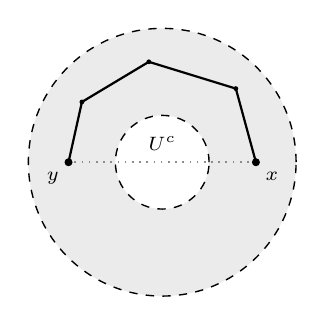
\begin{tikzpicture}[scale=1.7]
\fill[black!8, even odd rule] (0,0) circle (1) (0,0) circle (0.35);
\draw[black, dashed, line width=0.5pt] (0,0) circle (1);
\draw[black, dashed, line width=0.5pt] (0,0) circle (0.35);
\draw[black!45, dotted, line width=0.6pt] (0.7,0) -- (-0.7,0);
\draw[black, line width=0.8pt] (0.7,0) -- (0.55,0.55) -- (-0.1,0.75) -- (-0.6,0.45) -- (-0.7,0);
\foreach \p in {(0.55,0.55),(-0.1,0.75),(-0.6,0.45)} {\fill \p circle (0.018);}
\fill (0.7,0) circle (0.03); \fill (-0.7,0) circle (0.03);
\node[font=\scriptsize, below right] at (0.7,0) {$x$};
\node[font=\scriptsize, below left] at (-0.7,0) {$y$};
\node[font=\scriptsize] at (0,0.14) {$U^c$};
\end{tikzpicture}}{A polygonal path (solid) from $x$ to $y$ in the open annulus $U=\{z\in\mathbb R^2: 0.35<\|z\|<1\}$ (shaded; the dashed circles do not belong to $U$). The segment from $x$ to $y$ (dotted) leaves $U$, but a path with four segments stays inside. By \cref{thm:connected-open}, such paths exist between any two points of a connected open set.\label{fig:polygonal-path}}
\end{figure}

\begin{theorem}[Connected open sets]
\label{thm:connected-open}
For an open subset $U$ of a normed space the following are equivalent:
\begin{enumerate}
\item $U$ is connected;
\item $U$ is path-connected;
\item any two points of $U$ are joined by a polygonal path in $U$.
\end{enumerate}
\end{theorem}

\begin{proof}
(iii)$\Rightarrow$(ii) is clear, and (ii)$\Rightarrow$(i) is \cref{prop:path-connected}\,(i). (i)$\Rightarrow$(iii): Let $U$ be connected and nonempty, fix $a\in U$, and let $A$ be the set of points of $U$ that are joined to $a$ by a polygonal path in $U$. It contains $a$. If $x\in A$ and $B(x,r)\subseteq U$, every $y\in B(x,r)$ lies in $A$: append to a polygonal path from $a$ to $x$ the segment from $x$ to $y$, which lies in the convex set $B(x,r)$. So $A$ is open. If $x\in U\setminus A$ and $B(x,r)\subseteq U$, then no $y\in B(x,r)$ lies in $A$, since otherwise the segment from $y$ to $x$ would put $x$ in $A$; so $U\setminus A$ is open. By connectedness $U\setminus A$ is empty, and every point of $U$ is joined to $a$, hence, by reversing and joining paths, to every other point.
\end{proof}

For open subsets of $\mathbb R^n$, \vcref{1}{def:connected-open} called a set connected if any two of its points can be joined by a broken line, which is (iii). The theorem shows that this is connectedness in the sense of \cref{def:connected}, so that the remark after \vcref{1}{cor:zero-gradient} and the theorems of \vcref{1}{ch:vector-calculus} that assume connected open sets hold for all connected open sets in the present sense. The proof also shows that the segments can be taken parallel to the coordinate axes, since the cubes $\{y: \|y-x\|_\infty<r\}$ are open in $\mathbb R^n$ and any two of their points are joined by at most $n$ axis-parallel segments inside the cube.

The argument of the proof is worth isolating. A function $f$ on a metric space is \term{locally constant} if every point has a neighbourhood on which $f$ is constant.

\begin{proposition}[Locally constant functions]
\label{prop:locally-constant}
Every locally constant function on a connected metric space is constant. In particular, if $U\subseteq\mathbb R^n$ is open and connected and $f\colon U\to\mathbb R$ is differentiable with $\nabla f=\mathbf 0$ on $U$, then $f$ is constant.
\end{proposition}

\begin{proof}
Let $f$ be locally constant on $X$ and $a\in X$. The set $\{x: f(x)=f(a)\}$ is open, since each of its points has a neighbourhood on which $f$ equals $f(a)$, and its complement is open for the same reason. It is nonempty, so it is $X$, by \cref{prop:connected-characterisations}. For the second statement, every point of $U$ has a ball in $U$ around it, which is convex, and $f$ is constant on the ball by \vcref{1}{cor:zero-gradient}.
\end{proof}

On a disconnected open set the conclusion fails: on $\mathbb R\setminus\{0\}$ the function equal to $-1$ for $x<0$ and $1$ for $x>0$ has derivative $0$. The proposition is the general form of this observation, and it is how connectedness enters uniqueness theorems: the constant of integration of an antiderivative, a potential of a gradient field, or a solution of a differential equation determined by one value are unique only on connected domains.

\subsection{Totally Disconnected Sets}

A metric space is \term{totally disconnected} if its components are its one-point sets. We have seen that $\mathbb Q$ is totally disconnected, and the same argument applies to every subset of $\mathbb R$ that contains no interval of positive length: such a set has no connected subsets with two points. So the irrational numbers and the Cantor set are totally disconnected; the latter because it contains no interval, by \cref{prop:cantor-set}\,(ii). The space $\Omega=\{0,1\}^{\{1,2,\ldots\}}$ of \cref{sec:compact-continuous} is totally disconnected as well, since it is homeomorphic to the Cantor set, and connectedness, being defined by open sets, is preserved by homeomorphisms. The Cantor set is thus a nonempty compact metric space that is totally disconnected and has no isolated points, and Brouwer proved that every such space is homeomorphic to it~\cite[Thm.~7.4]{kechris1995}.

Connectedness also distinguishes spaces that cannot be told apart by cardinality. By \cref{thm:continuum-sets}, the line and the plane have the same number of points.

\begin{proposition}
\label{prop:line-plane}
The spaces $\mathbb R$ and $\mathbb R^2$ are not homeomorphic, and neither are $[0,1]$ and the unit circle $S^1$.
\end{proposition}

\begin{proof}
Suppose $h\colon\mathbb R^2\to\mathbb R$ is a homeomorphism and let $p\in\mathbb R^2$. Then $h$ restricts to a homeomorphism of $\mathbb R^2\setminus\{p\}$ onto $\mathbb R\setminus\{h(p)\}$. The first set is path-connected by \cref{prop:path-connected}\,(iv), translated by $p$, hence connected; the second is not, being the union of the disjoint nonempty open sets $(-\infty,h(p))$ and $(h(p),\infty)$. This contradicts \cref{thm:connected-image}. For $[0,1]$ and $S^1$, remove the point $1/2$ from the interval and its image from the circle: the interval falls into two pieces, while the circle without a point is the image of an open interval under $t\mapsto(\cos t,\sin t)$, hence connected.
\end{proof}

That $\mathbb R^m$ and $\mathbb R^n$ are not homeomorphic for $m\ne n$ is a deeper theorem of Brouwer, the invariance of dimension, which needs the methods of algebraic topology~\cite[Sect.~2.B]{hatcher2002}; removing points no longer helps for $m,n\ge2$.

\section{Paths in Matrix Groups}
\label{sec:matrix-paths}

The space $\mathbb F^{n\times n}$ of square matrices is a normed space of dimension $n^2$, and by \cref{thm:norms-equivalent} all its norms, the operator norms and the Frobenius norm among them, give the same open sets, convergent sequences, compact sets and connected sets. A sequence of matrices converges if and only if every entry converges, and a function of a matrix that is built from the entries by sums, products and quotients with nonzero denominators, such as the determinant, the adjugate and the inverse, is continuous. This section applies compactness and connectedness to sets of matrices. We write
\begin{gather*}
\mathrm{GL}_n(\mathbb F)\coloneqq\{A\in\mathbb F^{n\times n}: \det A\ne0\},\\
\mathrm O(n)\coloneqq\{Q\in\mathbb R^{n\times n}: Q^{\mathsf T}Q=I\},\qquad\mathrm U(n)\coloneqq\{Q\in\mathbb C^{n\times n}: Q^{\mathsf H}Q=I\}
\end{gather*}
for the invertible, the orthogonal and the unitary matrices, and $\mathrm{SO}(n)\coloneqq\{Q\in\mathrm O(n): \det Q=1\}$ for the rotations. All of them are groups under multiplication.

\subsection{Invertible Matrices Are Open and Dense}

\begin{proposition}
\label{prop:gl-open-dense}
$\mathrm{GL}_n(\mathbb F)$ is an open and dense subset of $\mathbb F^{n\times n}$.
\end{proposition}

\begin{proof}
It is open as the preimage of the open set $\mathbb F\setminus\{0\}$ under the continuous function $\det$, or by \cref{cor:perturbation-banach}, which gives the explicit ball $\{A+E: \|E\|<1/\|A^{-1}\|\}$ of invertible matrices around every invertible $A$. For density, let $A\in\mathbb F^{n\times n}$. The function $t\mapsto\det(A+tI)$ is a polynomial in $t$ of degree $n$ with leading coefficient $1$, so it has at most $n$ zeros (\vcref{1}{cor:factor}). Hence there are $t_k\to0$ with $\det(A+t_kI)\ne0$, and $A+t_kI\to A$.
\end{proof}

A random matrix is therefore invertible ``almost surely'', and a singular matrix becomes invertible under almost every small perturbation; this is why exact singularity is rarely seen in floating-point computation, and why the distance to the nearest singular matrix, $\sigma_n(A)$ in the $2$-norm by \vcref{2}{cor:distance-singular}, is the meaningful quantity. Density also justifies a method of proof that Volume~II used several times: an identity between continuous functions of matrices that holds for invertible matrices holds for all matrices, by \cref{prop:dense-agree}. Here is one more example.

\begin{proposition}
\label{prop:adjugate-product}
For all $A,B\in\mathbb F^{n\times n}$, $\operatorname{adj}(AB)=\operatorname{adj}(B)\operatorname{adj}(A)$.
\end{proposition}

\begin{proof}
For $n=1$ both sides are $[1]$ (\vcref{2}{def:adjugate}). Let $n\ge2$. Each entry of $\operatorname{adj}M$ is, up to sign, a minor of $M$, hence a polynomial in the entries of $M$; so both sides of the identity are continuous functions of the pair $(A,B)$ in $\mathbb F^{n\times n}\times\mathbb F^{n\times n}$. If $A$ and $B$ are invertible, then $\operatorname{adj}M=(\det M)M^{-1}$ for $M=A$, $B$ and $AB$, by \vcref{2}{thm:adjugate}, and
\[
\operatorname{adj}(AB)=\det(AB)\,(AB)^{-1}=\det B\,B^{-1}\det A\,A^{-1}=\operatorname{adj}(B)\operatorname{adj}(A).
\]
The pairs of invertible matrices form a dense subset of $\mathbb F^{n\times n}\times\mathbb F^{n\times n}$ with the product metric, by \cref{prop:gl-open-dense} applied to each factor, so the identity holds everywhere by \cref{prop:dense-agree}.
\end{proof}

A direct proof from the cofactors is possible, but requires the Cauchy--Binet formula for minors; the density argument replaces it by two lines. For complex matrices, the diagonalisable matrices, and even those with $n$ distinct eigenvalues, are dense in $\mathbb C^{n\times n}$, by \vcref{2}{thm:diagonalisable-dense}, and the paragraphs after that theorem used this to prove the Cayley--Hamilton theorem a third time. Over $\mathbb R$ this density fails. A real $2\times2$ matrix with the rows $(a,b)$ and $(c,d)$ has real eigenvalues if and only if its discriminant $\Delta\coloneqq(a-d)^2+4bc$ is nonnegative. The rotation $R_{\pi/2}$, with the rows $(0,-1)$ and $(1,0)$, has $\Delta=-4$, and since $\Delta$ is a continuous function of the entries, all matrices in a neighbourhood of $R_{\pi/2}$ have $\Delta<0$ and nonreal eigenvalues, so none of them is diagonalisable over $\mathbb R$. Such topological statements, that a property holds on an open set or on a dense set, are the precise form of the informal statements ``generically'' and ``robustly'' of numerical linear algebra.

\subsection{Matrices of Low Rank}

The same reasoning applies to rectangular matrices and their rank. By \vcref{2}{thm:rank-minors}, $\operatorname{rank}A\le k$ if and only if all minors of order $k+1$ vanish, and \vcref{2}{cor:rank-lsc} drew the consequence that the rank cannot drop under small perturbations. In topological language:

\begin{proposition}[Sets of matrices of bounded rank]
\label{prop:rank-sets}
Let $m,n\ge1$, $p\coloneqq\min(m,n)$ and $0\le k\le p$, and let $\mathcal R_k$ be the set of matrices in $\mathbb F^{m\times n}$ of rank at most $k$.
\begin{enumerate}
\item $\mathcal R_k$ is closed, and the set of matrices of full rank $p$ is open and dense in $\mathbb F^{m\times n}$.
\item $\mathcal R_k$ is the closure of the set of matrices of rank exactly $k$.
\item For every $A\in\mathbb F^{m\times n}$, the distance $\operatorname{dist}(A,\mathcal R_k)$ in any norm is attained by some matrix of rank at most $k$; in the norm $\|\cdot\|_2$ it equals $\sigma_{k+1}(A)$ for $k<p$.
\end{enumerate}
\end{proposition}

\begin{proof}
(i) For $k=p$ the set $\mathcal R_p$ is the whole space. For $k<p$, $\mathcal R_k$ is the set of common zeros of the minors of order $k+1$, which are polynomials in the entries and hence continuous; so it is an intersection of closed sets. The matrices of full rank form the complement of $\mathcal R_{p-1}$, which is open. For density and for (ii), let $A=\sum_{i=1}^r\sigma_i\mathbf u_i\mathbf v_i^{\mathsf H}$ be a singular value decomposition, with $r=\operatorname{rank}A$ and orthonormal $\mathbf u_1,\ldots,\mathbf u_p$ and $\mathbf v_1,\ldots,\mathbf v_p$ (\vcref{2}{thm:svd}). For $r\le j\le p$ and $t>0$, the matrix $A+t\sum_{i=r+1}^j\mathbf u_i\mathbf v_i^{\mathsf H}$ has the positive singular values $\sigma_1,\ldots,\sigma_r$ and $j-r$ values $t$, so its rank is $j$, and it tends to $A$ as $t\to0$. With $j=p$ this shows that the matrices of full rank are dense; with $j=k$, for $A\in\mathcal R_k$, it shows that $A$ is a limit of matrices of rank exactly $k$. Conversely, such limits lie in the closed set $\mathcal R_k$. (iii) $\mathcal R_k$ is a nonempty closed subset of the finite-dimensional space $\mathbb F^{m\times n}$, so a nearest point exists by \cref{cor:finite-dimensional}\,(vi); in the $2$-norm the distance is $\sigma_{k+1}$ by the Eckart--Young theorem, \vcref{2}{thm:eckart-young}.
\end{proof}

Part (i) is why numerical rank, rather than rank, is the meaningful notion in floating-point arithmetic, as \vcref{2}{prop:numerical-rank} made precise: a matrix of full rank stays of full rank under small perturbations, but every rank-deficient matrix is the limit of matrices of full rank, and rounding errors almost always produce one of them. The set $\mathcal R_k$ is not convex for $1\le k<p$, since $\mathbf e_1\mathbf e_1^{\mathsf T}$ and $\mathbf e_2\mathbf e_2^{\mathsf T}$ lie in $\mathcal R_1$ while their average has rank $2$; this is why the nearest matrices in (iii) need not be unique, as the theorem of Eckart and Young records for the spectral norm.

\subsection{The Two Components of the Real Invertible Matrices}

\Vcref{2}{prop:orientation-continuous} showed that a continuous path of bases cannot change the orientation, that is, that $\det$ cannot change its sign along a path in $\mathrm{GL}_n(\mathbb R)$. The note after it outlined the converse, that any two invertible matrices with determinants of the same sign can be joined by such a path. We now prove it, together with the corresponding statements for the orthogonal and unitary matrices.

\begin{theorem}[The orthogonal and unitary groups]
\label{thm:orthogonal-groups}
\leavevmode
\begin{enumerate}
\item $\mathrm O(n)$, $\mathrm{SO}(n)$ and $\mathrm U(n)$ are compact.
\item $\mathrm{SO}(n)$ and $\mathrm U(n)$ are path-connected.
\item $\mathrm O(n)$ has exactly two components, $\mathrm{SO}(n)$ and $\mathrm O^-(n)\coloneqq\{Q\in\mathrm O(n): \det Q=-1\}$, and each of them is path-connected.
\end{enumerate}
\end{theorem}

\begin{proof}
(i) The set $\mathrm O(n)$ is closed, since $Q\mapsto Q^{\mathsf T}Q$ is continuous, and bounded, since $\|Q\|_{\mathrm F}^2=\operatorname{tr}(Q^{\mathsf T}Q)=n$; it is compact by the Heine--Borel theorem. $\mathrm{SO}(n)$ is a closed subset of it, being a preimage of $\{1\}$ under $\det$, and $\mathrm U(n)$ is compact by the same argument as $\mathrm O(n)$.

(ii) Let $Q\in\mathrm{SO}(n)$. By \vcref{2}{cor:orthogonal-form}\,(i) there is an orthogonal $U$ with $U^{\mathsf T}QU=\operatorname{diag}(I_p,-I_q,R_{\varphi_1},\ldots,R_{\varphi_s})$, where $R_\varphi$ is the rotation through the angle $\varphi$ and $(-1)^q=\det Q=1$, so that $q$ is even. Since $-I_2=R_\pi$, the block $-I_q$ is a block diagonal matrix of $q/2$ rotations $R_\pi$, and we may write $U^{\mathsf T}QU=\operatorname{diag}(I_p,R_{\psi_1},\ldots,R_{\psi_l})$. Let
\[
Q_t\coloneqq U\operatorname{diag}\bigl(I_p,R_{(1-t)\psi_1},\ldots,R_{(1-t)\psi_l}\bigr)U^{\mathsf T}\qquad(0\le t\le1).
\]
Its entries are continuous functions of $t$, since those of $R_\theta$ are $\pm\cos\theta$ and $\pm\sin\theta$, and every $Q_t$ is orthogonal with determinant $1$. So $t\mapsto Q_t$ is a path in $\mathrm{SO}(n)$ from $Q_0=Q$ to $Q_1=I$. Any two rotations are joined through $I$. For a unitary $V$, there is a unitary $W$ with $V=W\operatorname{diag}(e^{i\theta_1},\ldots,e^{i\theta_n})W^{\mathsf H}$, $\theta_j\in\mathbb R$, because $V$ is normal (\vcref{2}{cor:schur-normal}) and its eigenvalues have modulus $1$ (\vcref{2}{prop:unitary-eigen}); and $V_t\coloneqq W\operatorname{diag}(e^{i(1-t)\theta_j})W^{\mathsf H}$ is a path in $\mathrm U(n)$ from $V$ to $I$.

(iii) Let $D\coloneqq\operatorname{diag}(-1,1,\ldots,1)$. Multiplication by $D$ maps $\mathrm{SO}(n)$ onto $\mathrm O^-(n)$ and back, and it is continuous, so $\mathrm O^-(n)$ is path-connected by \cref{prop:path-connected}\,(iii). The two sets are the preimages of the open sets $(0,\infty)$ and $(-\infty,0)$ under $\det$, since $\det Q=\pm1$ for orthogonal $Q$; so they are open in $\mathrm O(n)$, disjoint and nonempty, and they form a separation of $\mathrm O(n)$. Being connected, each lies in a component; and a component cannot meet both, since it is connected and would be separated by them. So they are the components.
\end{proof}

In $\mathrm{SO}(3)$, the path of the proof turns a rotation about an axis through the angle $\psi$ back to the identity by rotating through the angles $(1-t)\psi$ about the same axis (\vcref{2}{prop:rotation-axis}). A reflection in $\mathrm O^-(n)$ cannot be deformed into a rotation through orthogonal matrices, because the determinant would have to jump from $-1$ to $1$, and \cref{cor:ivt-general} forbids a continuous function on a connected set to omit the values in between.

\begin{theorem}[The real invertible matrices]
\label{thm:gl-real}
The set $\mathrm{GL}_n(\mathbb R)$ has exactly two components,
\[
\mathrm{GL}_n^+(\mathbb R)\coloneqq\{A: \det A>0\}\qquad\text{and}\qquad\mathrm{GL}_n^-(\mathbb R)\coloneqq\{A: \det A<0\},
\]
and each of them is open in $\mathbb R^{n\times n}$ and path-connected. Every $A\in\mathrm{GL}_n^+(\mathbb R)$ can be joined to $I$, and every $A\in\mathrm{GL}_n^-(\mathbb R)$ to $D=\operatorname{diag}(-1,1,\ldots,1)$, by a path of invertible matrices.
\end{theorem}

\begin{proof}
Let $A\in\mathrm{GL}_n^+(\mathbb R)$. Its columns are linearly independent, so by \vcref{2}{thm:qr} it has a QR factorisation $A=QR$ with an orthogonal $Q$ and an upper triangular $R$ with positive diagonal entries $r_{jj}$. Then $\det R=\prod_jr_{jj}>0$ and $\det Q=\det A/\det R>0$, so $Q\in\mathrm{SO}(n)$. For $0\le t\le1$ let $R_t\coloneqq(1-t)R+tI$. It is upper triangular with the positive diagonal entries $(1-t)r_{jj}+t$, hence invertible, and $t\mapsto QR_t$ is a path in $\mathrm{GL}_n^+(\mathbb R)$ from $A$ to $Q$. By \cref{thm:orthogonal-groups}\,(ii), $Q$ is joined to $I$ by a path in $\mathrm{SO}(n)\subseteq\mathrm{GL}_n^+(\mathbb R)$, and joining the two paths gives a path from $A$ to $I$. So $\mathrm{GL}_n^+(\mathbb R)$ is path-connected. Multiplication by $D$ is a continuous bijection of $\mathrm{GL}_n^+(\mathbb R)$ onto $\mathrm{GL}_n^-(\mathbb R)$, with itself as inverse, so $\mathrm{GL}_n^-(\mathbb R)$ is path-connected and every element is joined to $D=DI$. Both sets are open, as preimages of open sets under $\det$, disjoint and nonempty, so they form a separation of $\mathrm{GL}_n(\mathbb R)$, and as in the proof of \cref{thm:orthogonal-groups}\,(iii) they are its components.
\end{proof}

The proof makes the note of \vcref{2}{sec:det-volume} precise in a different way from the outline given there, which deformed the factors of a product of elementary matrices (\vcref{2}{cor:elementary-product}); both arguments are complete once paths and connectedness are defined, and the QR factorisation has the advantage that the path is given by a formula. It also shows more: the factorisation $A=QR$, whose factors depend continuously on $A$ by the formulas of the Gram--Schmidt process, identifies $\mathrm{GL}_n^+(\mathbb R)$ with the product of $\mathrm{SO}(n)$ and the set of upper triangular matrices with positive diagonal, which is convex, so that the real invertible matrices are, topologically, the orthogonal matrices together with a convex set of ``shapes''.

\subsection{The Complex Invertible Matrices}

Over $\mathbb C$ there is no orientation to preserve, and the invertible matrices form a single piece. The proof is a pleasant use of the fundamental fact that a nonzero polynomial has only finitely many zeros.

\begin{theorem}[The complex invertible matrices]
\label{thm:gl-complex}
$\mathrm{GL}_n(\mathbb C)$ is path-connected.
\end{theorem}

\begin{proof}
Let $A\in\mathrm{GL}_n(\mathbb C)$, and consider the matrices $(1-z)A+zI$ for $z\in\mathbb C$, on the complex line through $A$ and $I$. The function $p(z)\coloneqq\det\bigl((1-z)A+zI\bigr)$ is a polynomial in $z$ of degree at most $n$, by the Leibniz formula, and it is not the zero polynomial, since $p(1)=1$. So it has finitely many zeros $\zeta_1,\ldots,\zeta_m$ (\vcref{1}{cor:factor}), none of them equal to $0$ or $1$, since $p(0)=\det A\ne0$. Choose $w\in\mathbb C$ that lies on none of the finitely many rays from $0$ through a $\zeta_j$ and from $1$ through a $\zeta_j$; such $w$ exist, since a circle around $0$ of radius larger than $2$ meets each of these rays in at most one point. Then the segment from $0$ to $w$ and the segment from $w$ to $1$ avoid all zeros of $p$. Let $\gamma\colon[0,1]\to\mathbb C$ run along the first segment and then along the second, as in \cref{sec:connectedness}. The path $t\mapsto(1-\gamma(t))A+\gamma(t)I$ has continuous entries, starts at $A$, ends at $I$, and its determinant $p(\gamma(t))$ never vanishes.
\end{proof}

Over $\mathbb R$ the same idea fails, and it shows why. The segment from $A$ to $I$ is the real interval $0\le z\le1$, and if $\det A<0$, the real polynomial $p$, negative at $0$ and positive at $1$, has a zero in between by the intermediate value theorem; the detour through nonreal $z$ that saves the complex case is not available, because the matrices $(1-z)A+zI$ are then no longer real. Topologically, $\mathbb C$ without finitely many points is connected, while $\mathbb R$ without one point is not. The QR argument of \cref{thm:gl-real} gives a second proof: a complex invertible $A$ is $QR$ with a unitary $Q$ and an upper triangular $R$ with positive diagonal, $R$ is deformed into $I$ as before, and $Q$ into $I$ by \cref{thm:orthogonal-groups}\,(ii). Hall~\cite[Sect.~1.3]{hall2015} treats the topology of these and other matrix groups.

\section{The Baire Category Theorem}
\label{sec:baire}

Cardinality distinguishes countable sets from uncountable ones, and length, which Part~III develops into measure, distinguishes sets of length zero from larger ones. Completeness supplies a third notion of size, which is topological. A closed set without interior points, such as a line in the plane or the Cantor set in $\mathbb R$, is thin in the sense that every open set contains an open set that avoids it, and Baire's theorem says that a complete metric space is never a countable union of such thin sets. This is an existence theorem: to show that a point with some property exists, it suffices to show that the points without the property form a countable union of thin sets.

\subsection{Thin Sets}

\begin{definition}[Nowhere dense, meagre and residual sets]
\label{def:meagre}
Let $X$ be a metric space. A set $E\subseteq X$ is \term{nowhere dense} if its closure has empty interior, $\operatorname{int}\overline E=\emptyset$. It is \term{meagre}, or of the \term{first category}, if it is a countable union of nowhere dense sets, and of the \term{second category} otherwise. A set is \term{residual} if its complement is meagre. A countable intersection of open sets is a \term{$G_\delta$ set}, and a countable union of closed sets an \term{$F_\sigma$ set}.
\end{definition}

A set $E$ is nowhere dense if and only if every nonempty open set $U$ contains a nonempty open set that does not meet $E$, namely $U\setminus\overline E$, which is nonempty because $U\not\subseteq\overline E$. For a closed set $F$, being nowhere dense means having no interior points, and then $X\setminus F$ is open and dense. So the complement of a meagre set contains a countable intersection of dense open sets, and conversely a countable intersection of dense open sets has a meagre complement: residual sets are those that contain a countable intersection of dense open sets.

Finite sets are nowhere dense in $\mathbb R$, and so are $\mathbb Z$, the set $\{1/n: n\ge1\}$ and the Cantor set, which is closed and contains no interval. The set $\mathbb Q$ is not nowhere dense, since its closure is $\mathbb R$, but it is meagre, as a countable union of points. A line in the plane is nowhere dense, and so is the graph of a continuous function $\mathbb R\to\mathbb R$. In a normed space, every subspace $Y\ne X$ that is closed is nowhere dense: if it contained a ball $B(y,r)$, it would contain $B(0,r)=B(y,r)-y$ and hence, by scaling, all of $X$. In particular, every finite-dimensional subspace of an infinite-dimensional normed space is nowhere dense, by \cref{cor:finite-dimensional}\,(iii). The open set $\mathbb R\setminus\mathbb Z$ and the set of irrational numbers, $\bigcap_{q\in\mathbb Q}(\mathbb R\setminus\{q\})$, are $G_\delta$ sets; $\mathbb Q$ is an $F_\sigma$ set.

\subsection{Baire's Theorem}

\begin{theorem}[Baire category theorem]
\label{thm:baire}
Let $X$ be a complete metric space. The intersection of countably many dense open subsets of $X$ is dense in $X$. Equivalently: every meagre subset of $X$ has empty interior; and if $X\ne\emptyset$, then $X$ is not meagre in itself, so that $X$ is not a countable union of closed sets with empty interior.
\end{theorem}

\begin{proof}
Let $U_1,U_2,\ldots$ be dense open sets and $B_0\coloneqq B(x_0,r_0)$ an open ball, $r_0>0$. We find a point of $B_0$ that lies in every $U_n$. Since $U_1$ is dense, it meets $B_0$, and $B_0\cap U_1$ is open; choose a ball $B(x_1,\rho)\subseteq B_0\cap U_1$ and a radius $r_1$ with $0<r_1<\min(\rho,1)$, so that the closed ball $\bar B(x_1,r_1)$ lies in $B_0\cap U_1$. Recursively, given $x_{n-1}$ and $r_{n-1}$, the open set $B(x_{n-1},r_{n-1})\cap U_n$ is nonempty, because $U_n$ is dense, and we choose $x_n$ and $r_n$ with $0<r_n<1/n$ such that
\[
\bar B(x_n,r_n)\subseteq B(x_{n-1},r_{n-1})\cap U_n .
\]
The closed balls $\bar B(x_n,r_n)$ are nonempty, nested and have diameters at most $2r_n<2/n$, so by Cantor's intersection theorem, \cref{thm:cantor-intersection}, they have a common point $x$. It lies in $\bar B(x_1,r_1)\subseteq B_0$ and in $\bar B(x_n,r_n)\subseteq U_n$ for every $n$.

For the equivalent forms, let $M=\bigcup_nE_n$ with nowhere dense sets $E_n$. The sets $U_n\coloneqq X\setminus\overline{E_n}$ are open and dense, so $\bigcap_nU_n$ is dense, and it does not meet $M$. A set whose complement is dense has empty interior, so $M$ has empty interior; for $M=X\ne\emptyset$ this is impossible. Conversely, the first form follows from the second, since the complement of a countable intersection of dense open sets is meagre, and a set whose complement has empty interior is dense.
\end{proof}

This is the proof announced after Cantor's intersection theorem in \cref{sec:completeness-metric}: the balls are chosen to avoid one thin set after another, as \cref{fig:baire-balls} illustrates, and completeness provides a point that survives all the choices.

\begin{figure}
\sdfloat{%
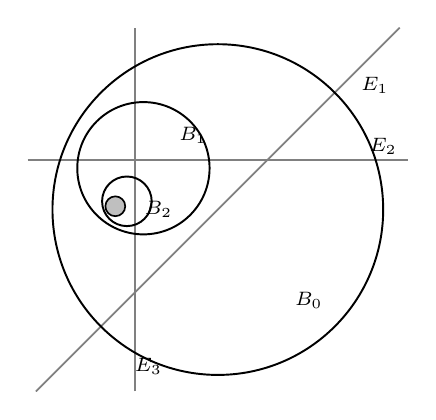
\begin{tikzpicture}[scale=2.1]
\clip (-1.15,-1.1) rectangle (1.15,1.1);
\draw[black!50, line width=0.6pt] (-1.1,-1.1) -- (1.1,1.1);
\draw[black!50, line width=0.6pt] (-1.15,0.3) -- (1.15,0.3);
\draw[black!50, line width=0.6pt] (-0.5,-1.1) -- (-0.5,1.1);
\draw[black, line width=0.7pt] (0,0) circle (1);
\draw[black, line width=0.7pt] (-0.45,0.25) circle (0.4);
\draw[black, line width=0.7pt] (-0.55,0.05) circle (0.15);
\fill[black!25] (-0.62,0.02) circle (0.06);
\draw[black, line width=0.6pt] (-0.62,0.02) circle (0.06);
\node[font=\scriptsize] at (0.55,-0.55) {$B_0$};
\node[font=\scriptsize] at (-0.15,0.45) {$B_1$};
\node[font=\scriptsize] at (-0.36,0.0) {$B_2$};
\node[font=\scriptsize] at (0.95,0.75) {$E_1$};
\node[font=\scriptsize] at (1.0,0.38) {$E_2$};
\node[font=\scriptsize] at (-0.42,-0.95) {$E_3$};
\end{tikzpicture}}{The proof of Baire's theorem in the plane, with three nowhere dense sets, the lines $E_1$, $E_2$ and $E_3$ (grey), and the dense open sets $U_n=\mathbb R^2\setminus E_n$. Inside the ball $B_0$, the closed ball $B_1$ avoids $E_1$, the closed ball $B_2\subseteq B_1$ avoids $E_2$, and the closed ball $B_3\subseteq B_2$ (shaded) avoids $E_3$. Continuing with countably many sets and radii tending to $0$, the balls shrink to a point that lies in none of the $E_n$.\label{fig:baire-balls}}
\end{figure} Completeness cannot be omitted. The space $\mathbb Q$ is the countable union of its points, each of which is closed and nowhere dense in $\mathbb Q$. The theorem also holds in every \term{locally compact} metric space, in which every point has a compact neighbourhood, such as an open subset of $\mathbb R^n$: in the proof, one chooses the first ball so small that its closure is compact, and replaces Cantor's intersection theorem by \cref{cor:nested-compact}. An open subset $U$ of a complete space $X$ is in general not complete, but it satisfies the conclusion as well: if $V_n$ are dense open subsets of $U$, the sets $V_n\cup(X\setminus\overline U)$ are dense and open in $X$, and every nonempty open subset of $U$ meets their intersection $\bigl(\bigcap_nV_n\bigr)\cup(X\setminus\overline U)$ in a point of $\bigcap_nV_n$.

A form of the theorem that is often convenient in applications concerns covers by closed sets.

\begin{corollary}[Closed covers]
\label{cor:baire-closed-cover}
Let $X$ be a complete metric space and $X=\bigcup_nF_n$ with closed sets $F_n$. Then the open set $\bigcup_n\operatorname{int}F_n$ is dense in $X$. In particular, if $X\ne\emptyset$, some $F_n$ contains a ball.
\end{corollary}

\begin{proof}
The set $F_n\setminus\operatorname{int}F_n$ is closed, as the intersection of $F_n$ with the closed set $X\setminus\operatorname{int}F_n$, and it has empty interior: an open set inside $F_n\setminus\operatorname{int}F_n$ would lie in $F_n$ and hence in $\operatorname{int}F_n$, by \cref{prop:closure}\,(i). So $E\coloneqq\bigcup_n(F_n\setminus\operatorname{int}F_n)$ is meagre, and $X\setminus E$ is dense by \cref{thm:baire}. A point $x\notin E$ lies in some $F_n$, because the $F_n$ cover $X$, and not in $F_n\setminus\operatorname{int}F_n$, so it lies in $\operatorname{int}F_n$. Hence $X\setminus E\subseteq\bigcup_n\operatorname{int}F_n$, and the latter is dense.
\end{proof}

\subsection{First Applications}

\begin{corollary}[Complete spaces without isolated points]
\label{cor:perfect-uncountable}
A nonempty complete metric space without isolated points is uncountable. In particular $\mathbb R$, every interval of positive length and the Cantor set are uncountable.
\end{corollary}

\begin{proof}
In a space without isolated points, every one-point set $\{x\}$ is closed and has empty interior, since an open set $\{x\}$ would contain a ball $B(x,r)=\{x\}$, which makes $x$ isolated. A countable space would be the countable union of its points, contradicting \cref{thm:baire}. The Cantor set is complete, as a closed subset of $\mathbb R$, and it has no isolated points by \cref{prop:cantor-set}\,(iii).
\end{proof}

This is the third proof in this series that $\mathbb R$ is uncountable, after the diagonal argument of \vcref{1}{thm:r-uncountable} and Cantor's nested interval argument, \cref{prop:cantor-nested}. The present proof is in fact a version of the latter: the nested intervals that avoid the points $x_0,x_1,\ldots$ one after another are the nested balls of the proof of Baire's theorem, which avoid the nowhere dense sets $\{x_n\}$. What Baire's theorem adds is that the same works for any countable family of nowhere dense sets, not only for points.

\begin{proposition}
\label{prop:q-not-gdelta}
The set $\mathbb Q$ is not a $G_\delta$ subset of $\mathbb R$, and the set of irrational numbers is not an $F_\sigma$ subset.
\end{proposition}

\begin{proof}
Suppose $\mathbb Q=\bigcap_nU_n$ with open sets $U_n$. Each $U_n$ contains $\mathbb Q$ and is therefore dense. So are the open sets $V_q\coloneqq\mathbb R\setminus\{q\}$, $q\in\mathbb Q$, of which there are countably many. The intersection of all the $U_n$ and all the $V_q$ is $\mathbb Q\cap(\mathbb R\setminus\mathbb Q)=\emptyset$, which contradicts \cref{thm:baire}. The second statement follows by taking complements.
\end{proof}

\subsection{Points of Continuity}

The note on functions with many discontinuities in \vcref{1}{sec:continuity} introduced Thomae's function, which is continuous at every irrational number and discontinuous at every rational one, and stated that no function is continuous exactly at the rational numbers. \Cref{fig:thomae} shows Thomae's function. To prove the statement, we measure how badly a function fails to be continuous at a point.

\begin{figure}
\sdfloat{%
\begin{tikzpicture}
\begin{axis}[sdplot, width=0.62\textwidth, height=0.36\textwidth, xmin=-0.02, xmax=1.02, ymin=0, ymax=1.06,
  xtick={0,0.5,1}, ytick={0,0.5,1}, xlabel={$x$}]
\addplot[black, only marks, mark=*, mark size=0.75pt] coordinates {(0.00000,1.00000) (1.00000,1.00000) (0.50000,0.50000) (0.33333,0.33333) (0.66667,0.33333) (0.25000,0.25000) (0.75000,0.25000) (0.20000,0.20000) (0.40000,0.20000) (0.60000,0.20000) (0.80000,0.20000) (0.16667,0.16667) (0.83333,0.16667) (0.14286,0.14286) (0.28571,0.14286) (0.42857,0.14286) (0.57143,0.14286) (0.71429,0.14286) (0.85714,0.14286) (0.12500,0.12500) (0.37500,0.12500) (0.62500,0.12500) (0.87500,0.12500) (0.11111,0.11111) (0.22222,0.11111) (0.44444,0.11111) (0.55556,0.11111) (0.77778,0.11111) (0.88889,0.11111) (0.10000,0.10000) (0.30000,0.10000) (0.70000,0.10000) (0.90000,0.10000) (0.09091,0.09091) (0.18182,0.09091) (0.27273,0.09091) (0.36364,0.09091) (0.45455,0.09091) (0.54545,0.09091) (0.63636,0.09091) (0.72727,0.09091) (0.81818,0.09091) (0.90909,0.09091) (0.08333,0.08333) (0.41667,0.08333) (0.58333,0.08333) (0.91667,0.08333) (0.07692,0.07692) (0.15385,0.07692) (0.23077,0.07692) (0.30769,0.07692) (0.38462,0.07692) (0.46154,0.07692) (0.53846,0.07692) (0.61538,0.07692) (0.69231,0.07692) (0.76923,0.07692) (0.84615,0.07692) (0.92308,0.07692) (0.07143,0.07143) (0.21429,0.07143) (0.35714,0.07143) (0.64286,0.07143) (0.78571,0.07143) (0.92857,0.07143) (0.06667,0.06667) (0.13333,0.06667) (0.26667,0.06667) (0.46667,0.06667) (0.53333,0.06667) (0.73333,0.06667) (0.86667,0.06667) (0.93333,0.06667) (0.06250,0.06250) (0.18750,0.06250) (0.31250,0.06250) (0.43750,0.06250) (0.56250,0.06250) (0.68750,0.06250) (0.81250,0.06250) (0.93750,0.06250) (0.05882,0.05882) (0.11765,0.05882) (0.17647,0.05882) (0.23529,0.05882) (0.29412,0.05882) (0.35294,0.05882) (0.41176,0.05882) (0.47059,0.05882) (0.52941,0.05882) (0.58824,0.05882) (0.64706,0.05882) (0.70588,0.05882) (0.76471,0.05882) (0.82353,0.05882) (0.88235,0.05882) (0.94118,0.05882) (0.05556,0.05556) (0.27778,0.05556) (0.38889,0.05556) (0.61111,0.05556) (0.72222,0.05556) (0.94444,0.05556) (0.05263,0.05263) (0.10526,0.05263) (0.15789,0.05263) (0.21053,0.05263) (0.26316,0.05263) (0.31579,0.05263) (0.36842,0.05263) (0.42105,0.05263) (0.47368,0.05263) (0.52632,0.05263) (0.57895,0.05263) (0.63158,0.05263) (0.68421,0.05263) (0.73684,0.05263) (0.78947,0.05263) (0.84211,0.05263) (0.89474,0.05263) (0.94737,0.05263) (0.05000,0.05000) (0.15000,0.05000) (0.35000,0.05000) (0.45000,0.05000) (0.55000,0.05000) (0.65000,0.05000) (0.85000,0.05000) (0.95000,0.05000) (0.04762,0.04762) (0.09524,0.04762) (0.19048,0.04762) (0.23810,0.04762) (0.38095,0.04762) (0.47619,0.04762) (0.52381,0.04762) (0.61905,0.04762) (0.76190,0.04762) (0.80952,0.04762) (0.90476,0.04762) (0.95238,0.04762) (0.04545,0.04545) (0.13636,0.04545) (0.22727,0.04545) (0.31818,0.04545) (0.40909,0.04545) (0.59091,0.04545) (0.68182,0.04545) (0.77273,0.04545) (0.86364,0.04545) (0.95455,0.04545) (0.04348,0.04348) (0.08696,0.04348) (0.13043,0.04348) (0.17391,0.04348) (0.21739,0.04348) (0.26087,0.04348) (0.30435,0.04348) (0.34783,0.04348) (0.39130,0.04348) (0.43478,0.04348) (0.47826,0.04348) (0.52174,0.04348) (0.56522,0.04348) (0.60870,0.04348) (0.65217,0.04348) (0.69565,0.04348) (0.73913,0.04348) (0.78261,0.04348) (0.82609,0.04348) (0.86957,0.04348) (0.91304,0.04348) (0.95652,0.04348) (0.04167,0.04167) (0.20833,0.04167) (0.29167,0.04167) (0.45833,0.04167) (0.54167,0.04167) (0.70833,0.04167) (0.79167,0.04167) (0.95833,0.04167) (0.04000,0.04000) (0.08000,0.04000) (0.12000,0.04000) (0.16000,0.04000) (0.24000,0.04000) (0.28000,0.04000) (0.32000,0.04000) (0.36000,0.04000) (0.44000,0.04000) (0.48000,0.04000) (0.52000,0.04000) (0.56000,0.04000) (0.64000,0.04000) (0.68000,0.04000) (0.72000,0.04000) (0.76000,0.04000) (0.84000,0.04000) (0.88000,0.04000) (0.92000,0.04000) (0.96000,0.04000) (0.03846,0.03846) (0.11538,0.03846) (0.19231,0.03846) (0.26923,0.03846) (0.34615,0.03846) (0.42308,0.03846) (0.57692,0.03846) (0.65385,0.03846) (0.73077,0.03846) (0.80769,0.03846) (0.88462,0.03846) (0.96154,0.03846) (0.03704,0.03704) (0.07407,0.03704) (0.14815,0.03704) (0.18519,0.03704) (0.25926,0.03704) (0.29630,0.03704) (0.37037,0.03704) (0.40741,0.03704) (0.48148,0.03704) (0.51852,0.03704) (0.59259,0.03704) (0.62963,0.03704) (0.70370,0.03704) (0.74074,0.03704) (0.81481,0.03704) (0.85185,0.03704) (0.92593,0.03704) (0.96296,0.03704) (0.03571,0.03571) (0.10714,0.03571) (0.17857,0.03571) (0.32143,0.03571) (0.39286,0.03571) (0.46429,0.03571) (0.53571,0.03571) (0.60714,0.03571) (0.67857,0.03571) (0.82143,0.03571) (0.89286,0.03571) (0.96429,0.03571) (0.03448,0.03448) (0.06897,0.03448) (0.10345,0.03448) (0.13793,0.03448) (0.17241,0.03448) (0.20690,0.03448) (0.24138,0.03448) (0.27586,0.03448) (0.31034,0.03448) (0.34483,0.03448) (0.37931,0.03448) (0.41379,0.03448) (0.44828,0.03448) (0.48276,0.03448) (0.51724,0.03448) (0.55172,0.03448) (0.58621,0.03448) (0.62069,0.03448) (0.65517,0.03448) (0.68966,0.03448) (0.72414,0.03448) (0.75862,0.03448) (0.79310,0.03448) (0.82759,0.03448) (0.86207,0.03448) (0.89655,0.03448) (0.93103,0.03448) (0.96552,0.03448) (0.03333,0.03333) (0.23333,0.03333) (0.36667,0.03333) (0.43333,0.03333) (0.56667,0.03333) (0.63333,0.03333) (0.76667,0.03333) (0.96667,0.03333)};
\end{axis}
\end{tikzpicture}}{Thomae's function on $[0,1]$, which is $1/q$ at a rational number $p/q$ in lowest terms and $0$ at the irrational numbers. The points $(p/q,1/q)$ are shown for $q\le30$. Near every point only finitely many dots lie above any given height, so the function is continuous where it vanishes, at the irrational numbers, and discontinuous at the rational ones; its oscillation at $p/q$ is $1/q$.\label{fig:thomae}}
\end{figure}

\begin{definition}[Oscillation]
\label{def:oscillation}
Let $f\colon X\to Y$ be a map between metric spaces. The \term{oscillation} of $f$ at $a\in X$ is
\[
\omega_f(a)\coloneqq\inf_{\delta>0}\operatorname{diam}f\bigl(B(a,\delta)\bigr)\in[0,\infty].
\]
\end{definition}

Thomae's function $t$ has the oscillation $\omega_t(p/q)=1/q$ at a rational number in lowest terms: every interval around $p/q$ contains irrational numbers, where $t=0$, and in a small enough interval the only values besides $0$ are smaller than $1/q$ or equal to $1/q$ at $p/q$ itself, by the argument of the note. At irrational points the oscillation is $0$.

\begin{proposition}[Oscillation and continuity]
\label{prop:oscillation}
Let $f\colon X\to Y$ be a map between metric spaces.
\begin{enumerate}
\item $f$ is continuous at $a$ if and only if $\omega_f(a)=0$.
\item For every $\varepsilon>0$, the set $\{x: \omega_f(x)<\varepsilon\}$ is open.
\item The set $C_f$ of points at which $f$ is continuous is a $G_\delta$ set, and the set of points at which $f$ is discontinuous is an $F_\sigma$ set.
\end{enumerate}
\end{proposition}

\begin{proof}
(i) If $f$ is continuous at $a$ and $\varepsilon>0$, some $\delta$ gives $f(B(a,\delta))\subseteq B(f(a),\varepsilon)$, a set of diameter at most $2\varepsilon$; so $\omega_f(a)=0$. Conversely, if $\omega_f(a)=0$ and $\varepsilon>0$, some $\delta$ gives $\operatorname{diam}f(B(a,\delta))<\varepsilon$, and then $d(f(x),f(a))<\varepsilon$ for $x\in B(a,\delta)$. (ii) If $\omega_f(a)<\varepsilon$, choose $\delta$ with $\operatorname{diam}f(B(a,\delta))<\varepsilon$. For $x\in B(a,\delta)$ the ball $B(x,\delta-d(x,a))$ lies in $B(a,\delta)$, so $\omega_f(x)<\varepsilon$; thus $B(a,\delta)$ lies in the set. (iii) By (i), $C_f=\bigcap_{k\ge1}\{x: \omega_f(x)<1/k\}$, an intersection of open sets by (ii). Its complement is a union of closed sets.
\end{proof}

\begin{theorem}[No function is continuous exactly at the rationals]
\label{thm:no-rational-continuity}
There is no function $f\colon\mathbb R\to\mathbb R$ that is continuous at every rational number and discontinuous at every irrational number.
\end{theorem}

\begin{proof}
The set of continuity points of such a function would be $\mathbb Q$, which is a $G_\delta$ set by \cref{prop:oscillation}\,(iii) and not a $G_\delta$ set by \cref{prop:q-not-gdelta}.
\end{proof}

This completes the note in \vcref{1}{sec:continuity}. The asymmetry between the rational and the irrational numbers is not one of size in the sense of cardinality alone: a set of continuity points must be a $G_\delta$ set, and if it is dense, it is residual by \cref{thm:baire}, so that its complement is meagre. The irrationals, which are the continuity points of Thomae's function, are a residual set, and the rationals, a meagre set, cannot be the set of continuity points of anything.

\subsection{Limits of Continuous Functions}

A pointwise limit of continuous functions need not be continuous, as the monomials $x^n$ on $[0,1]$ show, whose limit jumps at $1$. But it cannot be discontinuous everywhere.

\begin{theorem}[Pointwise limits of continuous functions]
\label{thm:baire-one}
Let $X$ be a complete metric space, and let $f_n\colon X\to\mathbb R$ be continuous functions that converge at every point to a function $f$. Then the set of points at which $f$ is continuous is a dense $G_\delta$ set; in particular it is residual and nonempty if $X\ne\emptyset$.
\end{theorem}

\begin{proof}
Fix $k\ge1$, and for $N\in\mathbb N$ let
\[
F_N\coloneqq\{x\in X: |f_m(x)-f_n(x)|\le1/k\text{ for all }m,n\ge N\} .
\]
Each $F_N$ is closed, as the intersection of the closed sets $\{|f_m-f_n|\le1/k\}$, and the $F_N$ cover $X$, because $(f_n(x))$ is a Cauchy sequence for every $x$. By \cref{cor:baire-closed-cover}, the open set $G_k\coloneqq\bigcup_N\operatorname{int}F_N$ is dense. Let $x\in\operatorname{int}F_N$. Letting $m\to\infty$ in the definition of $F_N$ gives $|f(y)-f_N(y)|\le1/k$ for all $y\in F_N$. Choose $\delta>0$ with $B(x,\delta)\subseteq F_N$ and $|f_N(y)-f_N(x)|<1/k$ for $y\in B(x,\delta)$, by the continuity of $f_N$. For such $y$,
\[
|f(y)-f(x)|\le|f(y)-f_N(y)|+|f_N(y)-f_N(x)|+|f_N(x)-f(x)|<3/k ,
\]
so $\operatorname{diam}f(B(x,\delta))\le6/k$, and $\omega_f(x)\le6/k$. Thus $\omega_f\le6/k$ on $G_k$, and $\omega_f=0$ on $\bigcap_kG_k$, which is dense by \cref{thm:baire}. So the set $C_f$ of continuity points contains a dense $G_\delta$ set; it is dense, it is a $G_\delta$ set by \cref{prop:oscillation}, and it is residual.
\end{proof}

Functions that are pointwise limits of continuous functions are called functions of \term{Baire class one}. The Dirichlet function $\mathbf 1_{\mathbb Q}$ is discontinuous everywhere, so by the theorem it is not of this class, although it is a limit of such functions, since $\mathbf 1_{\mathbb Q}(x)=\lim_m\lim_n(\cos(m!\,\pi x))^{2n}$: for fixed $m$, the inner limit is $1$ if $m!\,x$ is an integer and $0$ otherwise. Baire classified functions by the number of limits needed to obtain them from continuous ones. Derivatives are of class one.

\begin{corollary}[Continuity points of derivatives]
\label{cor:derivative-continuity}
If $f$ is differentiable on an open interval $I$, then $f'$ is continuous at the points of a dense subset of $I$.
\end{corollary}

\begin{proof}
Let $[c,d]\subseteq I$ with $c<d$, and choose $h_0>0$ with $d+h_0\in I$. The functions $g_n(x)\coloneqq n\bigl(f(x+1/n)-f(x)\bigr)$, for $n>1/h_0$, are continuous on $[c,d]$, because $f$ is, and they converge to $f'(x)$ at every $x\in[c,d]$. By \cref{thm:baire-one}, applied in the complete space $[c,d]$, the restriction of $f'$ to $[c,d]$ is continuous at the points of a dense subset of $[c,d]$; at the points of $(c,d)$, continuity of the restriction is continuity of $f'$. Every open subinterval of $I$ contains such an interval $(c,d)$.
\end{proof}

The function $x^2\sin(1/x)$ of \vcref{1}{prop:x2sin} has a derivative that is discontinuous at $0$, and Darboux's theorem, \vcref{1}{thm:darboux}, shows that derivatives have the intermediate value property even when they are discontinuous. The corollary adds that a derivative cannot be discontinuous on an interval: its discontinuities form a meagre set. Volterra's function, mentioned in the note on derivatives in \vcref{1}{sec:darboux}, has a derivative whose discontinuities form a set of positive length that is nevertheless nowhere dense, which shows how far the corollary is from saying that the discontinuities are few in the sense of length.

\subsection{Hamel Bases of Banach Spaces}

The note on bases of infinite-dimensional spaces in \vcref{2}{sec:basis-dimension} described Hamel bases, in which every vector is a finite combination of basis vectors, and remarked that the bases that matter in analysis are of a different kind. Baire's theorem shows that Hamel bases of Banach spaces are always large.

\begin{theorem}[Hamel bases of Banach spaces]
\label{thm:hamel-uncountable}
An infinite-dimensional Banach space has no countable Hamel basis. Consequently, a normed space of countably infinite dimension, such as the space of polynomials with any norm or $c_{00}$ with any norm, is not complete.
\end{theorem}

\begin{proof}
Suppose $b_1,b_2,\ldots$ is a countable Hamel basis of the Banach space $X$; since $X$ is infinite-dimensional, the basis is infinite. Every vector is a finite combination of basis vectors, so $X=\bigcup_nY_n$ with $Y_n\coloneqq\operatorname{span}\{b_1,\ldots,b_n\}$. Each $Y_n$ is finite-dimensional, hence closed by \cref{cor:finite-dimensional}\,(iii), and different from $X$, hence nowhere dense, as observed after \cref{def:meagre}. This contradicts \cref{thm:baire}. The second statement is the contrapositive.
\end{proof}

The space $c_{00}$ of finite sequences thus fails to be complete not only in the norms $\|\cdot\|_p$, as \cref{sec:completeness-metric} showed, but in every norm whatsoever. The spaces of polynomials, of trigonometric polynomials and of finite sequences, which are the spaces on which computation actually takes place, are never complete; their completions, such as $C[a,b]$, $\ell^p$ and the spaces $L^p$ of Part~III, have uncountable Hamel bases, which cannot be written down and play no role in computation. Their useful bases are bases in the sense of convergent series, as the note in Volume~II said.

\begin{note}{Hamel bases and discontinuous additive functions}
By the axiom of choice, $\mathbb R$ regarded as a vector space over $\mathbb Q$ has a Hamel basis $H$, as Hamel showed~\cite{hamel1905}. It is uncountable: otherwise every real number would be a rational combination of finitely many elements of a countable set, and $\mathbb R$ would be countable, contrary to \cref{cor:perfect-uncountable}. Choose two basis elements $h_0\ne h_1$, and define $f\colon\mathbb R\to\mathbb R$ as the $\mathbb Q$-linear map with $f(h_0)=1$ and $f(h)=0$ for every other $h\in H$. Then $f(x+y)=f(x)+f(y)$ for all real $x$ and $y$, but $f$ is not of the form $f(x)=cx$: this would require $c=1/h_0$ and $ch_1=0$. By \vcref{1}{thm:cauchy-functional}, which shows that continuous additive functions are linear, $f$ is discontinuous; in fact it is discontinuous everywhere, and its graph is dense in the plane. For the latter, observe that the graph is a $\mathbb Q$-linear subspace of $\mathbb R^2$ that contains $(h_0,1)$ and $(h_1,0)$, and therefore all the points $s(h_0,1)+t(h_1,0)$ with $s,t\in\mathbb Q$. These points are the image of the dense set $\mathbb Q^2$ under the linear map with the matrix that has the columns $(h_0,1)$ and $(h_1,0)$, whose determinant $-h_1$ is nonzero; an invertible linear map of $\mathbb R^2$ is a homeomorphism and maps dense sets to dense sets. A function with a dense graph is unbounded on every interval, and so it is continuous nowhere. This is the construction of discontinuous additive functions mentioned in \vcref{1}{sec:general-powers} and in the note of \vcref{2}{sec:basis-dimension}. It cannot be made explicit, since it depends on the axiom of choice through the basis $H$; additive functions that are bounded on some interval, or merely measurable, are linear, as Acz\'el explains~\cite{aczel1966}.
\end{note}

\subsection{Category and Measure}

Meagre sets are small in the sense of category, and sets that can be covered by countably many intervals of arbitrarily small total length, the sets of measure zero of the note on Lebesgue's criterion in \vcref{1}{sec:integrable-functions}, are small in the sense of measure. The two notions of smallness are independent: a set can be small in one sense and large in the other. The Liouville numbers of \cref{sec:continuum} give an explicit example. Call an irrational number $x$ a \term{Liouville number} if for every $n\ge1$ there are integers $p$ and $q\ge2$ with
\[
0<\Bigl|x-\frac pq\Bigr|<\frac1{q^n} .
\]
Every Liouville number is transcendental, by \cref{thm:liouville}: if $x$ were algebraic of degree $d$, the inequality $c/q^d\le|x-p/q|<q^{-n}$ would force $q^{n-d}<1/c$, so for $n>d$ the denominators would satisfy $q<1/c$. But only finitely many fractions with denominators below $1/c$ lie within distance $1$ of $x$, none of them equals the irrational number $x$, and so their distances from $x$ have a positive minimum, which the bound $|x-p/q|<q^{-n}\le2^{-n}$ undercuts for large $n$.

\begin{proposition}[The Liouville numbers]
\label{prop:liouville-residual}
The set $L$ of Liouville numbers is a dense $G_\delta$ subset of $\mathbb R$, hence residual and uncountable, and it has measure zero: for every $\varepsilon>0$ it can be covered by countably many open intervals of total length less than $\varepsilon$.
\end{proposition}

\begin{proof}
For $n\ge1$ let
\[
U_n\coloneqq\bigcup_{q\ge2}\ \bigcup_{p\in\mathbb Z}\Bigl(\frac pq-\frac1{q^n},\frac pq+\frac1{q^n}\Bigr),
\]
an open set that contains every rational number, since $p/q=2p/(2q)$ can always be written with a denominator at least $2$; so $U_n$ is dense. An irrational $x$ lies in $U_n$ exactly when it has an approximation as in the definition for this $n$, so $L=(\mathbb R\setminus\mathbb Q)\cap\bigcap_nU_n$, which is a countable intersection of dense open sets, as $\mathbb R\setminus\mathbb Q=\bigcap_{r\in\mathbb Q}(\mathbb R\setminus\{r\})$. By \cref{thm:baire} it is dense and residual, and it is uncountable, since a countable set is meagre and $\mathbb R$ is not the union of two meagre sets.

For the measure, it suffices to cover $L\cap[m,m+1]$ for each integer $m$ by intervals of total length less than $\varepsilon/2^{|m|+2}$; together these cover $L$ with total length less than $\sum_m\varepsilon/2^{|m|+2}<\varepsilon$. By translation we may take $m=0$. For $n\ge3$, $L\cap[0,1]\subseteq U_n\cap[0,1]$, and the intervals of $U_n$ that meet $[0,1]$ have $0\le p\le q$, at most $q+1\le2q$ of them for each $q$, each of length $2q^{-n}$. Their total length is at most
\[
\sum_{q\ge2}2q\cdot2q^{-n}=4\sum_{q\ge2}q^{1-n}\le4\int_1^\infty x^{1-n}\,dx=\frac4{n-2},
\]
by comparison with the integral (\vcref{1}{thm:integral-test}), and this is less than any prescribed positive number for large $n$.
\end{proof}

So $\mathbb R$ is the union of the residual set $L$, which has measure zero, and its complement, which is meagre. Almost every real number, in the sense of measure, is not a Liouville number; a ``typical'' real number, in the sense of category, is one. Oxtoby's book is devoted to the interplay of the two notions~\cite{oxtoby1980}, and Part~III returns to measure. Chapter~5 uses Baire's theorem in the space $C[0,1]$ to prove that a typical continuous function, in the sense of category, is nowhere differentiable, a statement about functions that has no counterpart in the sense of measure at the level of this volume.

\section{Compactness and Dimension in Computation}
\label{sec:compact-computation}

The theorems of this chapter are qualitative: all norms on $\mathbb R^n$ are equivalent, a compact set has a finite $\varepsilon$-net, a closed bounded set in $\mathbb R^n$ is compact. Behind each of them stands a number that depends on the dimension, the constant of equivalence or the size of the net, and in the high dimensions of scientific computing these numbers are large. This section looks at them in three computations. They were made on an Apple M4 Pro processor with Python~3.15 and its binary64 floating-point numbers, using the random number generator, the normal distribution, the vector norms and the array operations of the version of the stardust library of 25 November 2026; the iteration counts of \cref{tab:jacobi-stopping} were reproduced independently with NumPy~2.5.5.

\subsection{Norms of Random Vectors}

On $\mathbb R^n$, $\|x\|_\infty\le\|x\|_1\le n\|x\|_\infty$ and $\|x\|_\infty\le\|x\|_2\le\sqrt n\,\|x\|_\infty$, and the upper constants are attained only by vectors whose components all have the same modulus. Are they a pessimistic artefact, or do typical vectors come close to them? \Cref{tab:norm-ratios} shows the ratios for vectors whose components are independent standard normal random numbers, $1000$ vectors for each dimension up to $10^4$ and $200$ for $n=10^5$.

\begin{table}
\sdfloat{%
\begin{sdtable}{colspec={rllll}, row{1}={font=\small\bfseries}}
\toprule
$n$ & $\|x\|_1/\|x\|_\infty$ & bound $n$ & $\|x\|_2/\|x\|_\infty$ & bound $\sqrt n$ \\
\midrule
$10$ & $4.31$ \ $[2.17,\,7.06]$ & $10$ & $1.66$ \ $[1.10,\,2.42]$ & $3.16$ \\
$10^2$ & $29.4$ \ $[17.6,\,41.2]$ & $10^2$ & $3.67$ \ $[2.40,\,5.02]$ & $10$ \\
$10^3$ & $235$ \ $[173,\,311]$ & $10^3$ & $9.34$ \ $[6.87,\,12.2]$ & $31.6$ \\
$10^4$ & $2003$ \ $[1430,\,2350]$ & $10^4$ & $25.1$ \ $[17.9,\,29.5]$ & $100$ \\
$10^5$ & $17\,748$ \ $[14\,374,\,19\,788]$ & $10^5$ & $70.3$ \ $[57.0,\,78.5]$ & $316$ \\
\bottomrule
\end{sdtable}}{Ratios of norms of random vectors $x\in\mathbb R^n$ with independent standard normal components: the median over the samples, followed by the smallest and the largest value in brackets, compared with the largest possible values $n$ and $\sqrt n$ of the ratios. The medians grow almost in proportion to the bounds.\label{tab:norm-ratios}}
\end{table}

The ratios are far from the lower bound $1$, which only vectors with a single nonzero component attain, and they grow almost as fast as the upper bounds. The reason is that a sum of $n$ comparable terms is about $n$ times a typical term, while the largest term grows very slowly with $n$. In the samples, the median of $\|x\|_1/n$ lay between $0.797$ and $0.798$ for every $n\ge100$, close to the mean $\sqrt{2/\pi}=0.7979$ of $|X|$ for a standard normal $X$, while the median of $\|x\|_\infty$ was $1.84$, $2.71$, $3.38$, $3.98$ and $4.49$ for $n=10,\ldots,10^5$, growing by less than $0.7$ for each factor $10$ from $n=100$ on. For $n=10^5$, the median ratio $\|x\|_1/\|x\|_\infty$ is $0.177n$, and $\|x\|_2/\|x\|_\infty$ is $0.222\sqrt n$. So the constants of equivalence are not an artefact: for vectors whose information is spread over all components, a tolerance in the norm $\|\cdot\|_1$ corresponds to a tolerance in $\|\cdot\|_\infty$ that is smaller by a factor growing almost in proportion to $n$.

\subsection{Stopping an Iteration}

The effect on an iterative method is easy to predict with \cref{prop:rate-norm-independent}. We ran Jacobi's method for the tridiagonal system of \cref{sec:metric-computation}, with $3$ on the diagonal and $-1$ next to it, now of size $n\in\{10^2,10^4,10^6\}$, with the right-hand side $b_i=1+\sin(\pi t_i)$ at $n$ equally spaced points $t_i$ of $[0,1]$, including the ends, from $\mathbf x_0=\mathbf 0$. By \cref{thm:jacobi-contraction}, the iteration contracts with $q=2/3$ in the norm $\|\cdot\|_\infty$. The iteration was stopped at the first step $k$ at which the step $\mathbf d_k\coloneqq\mathbf x_k-\mathbf x_{k-1}$ satisfied $\|\mathbf d_k\|\le10^{-8}$, for five choices of the norm. \Cref{tab:jacobi-stopping} shows the results.

\begin{table}
\sdfloat{%
\begin{sdtable}{colspec={rrrrrr}, row{1}={font=\small\bfseries}}
\toprule
$n$ & $\|\cdot\|_\infty$ & $\|\cdot\|_2$ & $\|\cdot\|_1$ & $n^{-1/2}\|\cdot\|_2$ & $n^{-1}\|\cdot\|_1$ \\
\midrule
$10^2$ & $46$ & $51$ & $57$ & $45$ & $45$ \\
$10^4$ & $46$ & $57$ & $68$ & $45$ & $45$ \\
$10^6$ & $46$ & $63$ & $80$ & $45$ & $45$ \\
\bottomrule
\end{sdtable}}{The number of Jacobi steps after which the step $\mathbf x_k-\mathbf x_{k-1}$ first has the norm at most $10^{-8}$, for the tridiagonal systems of the text and five norms. The last two columns use the norms divided by $n^{1/2}$ and $n$, which measure the root mean square and the mean modulus of the components.\label{tab:jacobi-stopping}}
\end{table}

In the maximum norm the number of steps does not depend on $n$; the iteration contracts by the factor $2/3$ per step, independently of the size of the system, as the theorem asserts. In the norms $\|\cdot\|_2$ and $\|\cdot\|_1$ the number grows by $5$, $11$, $17$ steps and by $11$, $22$, $34$ steps. The prediction of \cref{prop:rate-norm-independent} is that the extra number of steps is at most $\ln C/\ln(1/q)$, where $C$ is the constant in $\|\mathbf d\|\le C\|\mathbf d\|_\infty$, that is, $\ln\sqrt n/\ln(3/2)$ and $\ln n/\ln(3/2)$; these are $5.7$, $11.4$, $17.0$ and $11.4$, $22.7$, $34.1$. The observed numbers come within one step of the worst case, because the steps $\mathbf d_k$ have the shape of the right-hand side, spread evenly over all components: at $k=46$, $\|\mathbf d_k\|_1/(n\|\mathbf d_k\|_\infty)$ was $0.818$ for $n=10^6$, which is the ratio $(1+2/\pi)/2$ of the mean of $1+\sin\pi t$ over $[0,1]$ to its maximum. The last two columns show the remedy that numerical software commonly adopts: a tolerance for the root mean square or the mean modulus of the components, $n^{-1/2}\|\cdot\|_2$ or $n^{-1}\|\cdot\|_1$, has the same meaning in every dimension, and the number of steps is then independent of $n$. Whichever norm is chosen, the a posteriori bound of \cref{thm:banach-fixed-point} converts the step into a bound for the error, and the constants of equivalence convert it into another norm.

\subsection{Counting \texorpdfstring{$\varepsilon$}{epsilon}-Nets}

Total boundedness asks for a finite $\varepsilon$-net, and its size measures how much information is needed to describe a point of the set to within $\varepsilon$. For the unit ball of $\mathbb R^d$ the size can be estimated by volumes. Call a set $S$ \term{$\varepsilon$-separated} if any two of its points have a distance at least $\varepsilon$.

\begin{proposition}[Nets in the Euclidean ball]
\label{prop:covering-numbers}
Let $B$ be the closed Euclidean unit ball of $\mathbb R^d$ and $0<\varepsilon\le1$. Let $N(\varepsilon)$ be the smallest number of points of an $\varepsilon$-net of $B$, and let $P(\varepsilon)$ be the largest number of points of an $\varepsilon$-separated subset of $B$. Then
\[
\Bigl(\frac1\varepsilon\Bigr)^d\le N(\varepsilon)\le P(\varepsilon)\le\Bigl(1+\frac2\varepsilon\Bigr)^d .
\]
\end{proposition}

\begin{proof}
Let $V_d$ be the volume of $B$, so that a ball of radius $r$ has the volume $V_dr^d$, by \vcref{1}{thm:ball-volume}; an open ball has the same volume as the closed one, since they differ by a set of content zero. If $S\subseteq B$ is $\varepsilon$-separated, the open balls $B(s,\varepsilon/2)$, $s\in S$, are disjoint and lie in the ball of radius $1+\varepsilon/2$ around $0$. So $\sum_{s\in S}\mathbf 1_{B(s,\varepsilon/2)}\le\mathbf 1_{\bar B(0,1+\varepsilon/2)}$ pointwise, and integrating, with the linearity and monotonicity of the integral in $\mathbb R^d$ (\vcref{1}{thm:multiple-summary}), gives $|S|\,V_d(\varepsilon/2)^d\le V_d(1+\varepsilon/2)^d$, which is the upper bound for $P(\varepsilon)$. In particular $P(\varepsilon)$ is finite. An $\varepsilon$-separated set $S$ with $P(\varepsilon)$ points is an $\varepsilon$-net of $B$: a point of $B$ at a distance at least $\varepsilon$ from all points of $S$ could be added to $S$. So $N(\varepsilon)\le P(\varepsilon)$. Finally, if the balls $B(y_j,\varepsilon)$, $j=1,\ldots,N$, cover $B$, then $\mathbf 1_B\le\sum_j\mathbf 1_{B(y_j,\varepsilon)}$, and integrating gives $V_d\le NV_d\varepsilon^d$.
\end{proof}

Both bounds grow exponentially with the dimension. To see where the truth lies between them, we chose $10^6$ points independently and uniformly distributed in $B$, for $d=1,\ldots,10$, each as a normal random vector divided by its norm and multiplied by $u^{1/d}$ with $u$ uniform in $[0,1]$, and selected from them greedily a $1/2$-separated set: take the first point, discard all points closer than $1/2$ to it, and repeat with the first remaining point. The selected set is $1/2$-separated, as a final check of all pairwise distances confirmed, so its size is a lower bound for $P(1/2)$; and it is a $1/2$-net of the sample, though not necessarily of $B$. \Cref{fig:nets} shows the sizes together with the bounds $2^d$ and $5^d$ of the proposition.

\begin{figure}
\sdfloat{%
\begin{tikzpicture}
\begin{axis}[sdplot, width=0.56\textwidth, height=0.44\textwidth, ymode=log, xmin=0.5, xmax=10.5, ymin=1, ymax=2e7,
  xtick={1,2,...,10}, ytick={1,10,100,1000,10000,100000,1000000,10000000}, xlabel={$d$},
  legend style={at={(0.03,0.97)}, anchor=north west}]
\addplot[black!45, line width=0.7pt, mark=none] coordinates {(1,5) (2,25) (3,125) (4,625) (5,3125) (6,15625) (7,78125) (8,390625) (9,1953125) (10,9765625)};
\addlegendentry{$5^d$}
\addplot[black, line width=0.7pt, mark=*, mark size=1.4pt] coordinates {(1,4) (2,12) (3,38) (4,107) (5,271) (6,667) (7,1529) (8,3339) (9,6979) (10,14139)};
\addlegendentry{greedy}
\addplot[black, dashed, line width=0.7pt, mark=none] coordinates {(1,2) (2,4) (3,8) (4,16) (5,32) (6,64) (7,128) (8,256) (9,512) (10,1024)};
\addlegendentry{$2^d$}
\end{axis}
\end{tikzpicture}}{Sizes of $1/2$-separated sets in the unit ball of $\mathbb R^d$ selected greedily from $10^6$ random points (dots), for $d=1,\ldots,10$, with the lower bound $2^d$ for the size of a $1/2$-net and the upper bound $5^d$ for the size of a $1/2$-separated set from \cref{prop:covering-numbers}. The greedy sets grow by a factor between $2$ and $3$ per dimension, from $4$ points for $d=1$ to $14\,139$ for $d=10$.\label{fig:nets}}
\end{figure}

The greedy sets had $4$, $12$, $38$, $107$, $271$, $667$, $1529$, $3339$, $6979$ and $14\,139$ points. In dimension $1$ the largest $1/2$-separated subset of $[-1,1]$ has the $5$ points $-1,-1/2,0,1/2,1$, which attain the upper bound, while the greedy choice from random points found $4$. The ratio of successive sizes decreases from $3$ to about $2$, partly because $10^6$ random points become sparse in a ten-dimensional ball, so that the greedy set underestimates $P(1/2)$ more and more. The trend is unmistakable. To describe every point of the unit ball of $\mathbb R^{10}$ to within $1/2$, at least $2^{10}=1024$ reference points are needed, by the proposition; to within $1/4$, at least $14\,139$ are needed, since a ball of radius $1/4$ contains at most one point of a $1/2$-separated set; and for a tolerance $\varepsilon$ the number grows like $\varepsilon^{-d}$. This growth is one form of the curse of dimensionality, and it limits grid searches as in \vcref{1}{prop:grid-max}, which on $[0,1]^d$ need of the order of $(K\sqrt d/(2\varepsilon))^d$ evaluations to locate a maximum of a Lipschitz function with the constant $K$ to within $\varepsilon$, and nearest-neighbour searches, which Volume~XVII studies. In the limit of infinite dimension the count is infinite: the unit ball of $\ell^2$ contains the infinitely many unit sequences $\mathbf e_k$ at mutual distances $\sqrt2$, which is the noncompactness of \cref{prop:l2-ball-not-compact,thm:riesz-compact}.

\bigskip
A metric space is compact if every open cover has a finite subcover, and for metric spaces this is equivalent to sequential compactness and to completeness together with total boundedness; compact sets are closed and bounded, and in $\mathbb R^n$, by the Heine--Borel theorem, the closed bounded sets are exactly the compact ones, while the closed unit ball of $\ell^2$ is not compact. Finite and countable products of compact spaces are compact, and so are the Hilbert cube and the Cantor set, which is homeomorphic to the space of sequences of zeros and ones. Continuous images of compact sets are compact; continuous real functions on compact sets attain their extreme values, lower semicontinuous ones their minima; continuous maps on compact sets are uniformly continuous, and continuous bijections of compact sets are homeomorphisms. On a finite-dimensional space all norms are equivalent, so that finite-dimensional normed spaces are complete, their subspaces closed, their linear maps bounded and their closed bounded sets compact, and best approximations from finite-dimensional subspaces exist; by Riesz's lemma the closed unit ball is compact only in finite dimensions. A space is connected if it cannot be split into two disjoint nonempty open sets; the connected subsets of $\mathbb R$ are the intervals, continuous images of connected sets are connected, which is the general intermediate value theorem, open subsets of $\mathbb R$ are countable disjoint unions of open intervals, and connected open subsets of normed spaces are polygonally connected, although connected sets in general need not be path-connected. The real invertible matrices form two path components, distinguished by the sign of the determinant, and the complex ones a single one. In a complete metric space a countable intersection of dense open sets is dense; consequently such a space without isolated points is uncountable, no function is continuous exactly at the rational numbers, pointwise limits of continuous functions are continuous on a residual set, and infinite-dimensional Banach spaces have uncountable Hamel bases.

The next chapter studies sequences of functions and the uniform convergence that preserves continuity, integrals and, under conditions, derivatives. Compactness enters there through Dini's theorem and through the space $C(K)$ of continuous functions on a compact set, whose compact subsets Chapter~5 characterises.

\chapternotes

The idea of extracting finite subcovers grew out of the proofs of uniform continuity and of the theorems on continuous functions on closed intervals. Heine's paper of 1872 proved that continuous functions on closed intervals are uniformly continuous~\cite{heine1872}, and Borel proved in his thesis of 1895 that every countable cover of a closed bounded interval by open intervals has a finite subcover~\cite{borel1895}; the extension to arbitrary covers is due to Cousin~\cite{cousin1895} and to Lebesgue. Fr\'echet introduced the word ``compact'' in his thesis~\cite{frechet1906}, for sets in which every infinite subset has an accumulation point, and the definition by open covers became standard through the work of Alexandroff and Urysohn in the 1920s. Raman-Sundstr\"om traces this history and its consequences for teaching~\cite{ramansundstrom2015}. Hausdorff's \emph{Grundz\"uge der Mengenlehre} introduced total boundedness and proved that a metric space is compact if and only if it is complete and totally bounded~\cite{hausdorff1914}. Tychonoff's theorem on products is in~\cite{tychonoff1930}, and Riesz's lemma and the theorem that the unit ball is compact only in finite dimensions are in his paper of 1918 on linear functional equations~\cite{riesz1918}, which also laid the foundations of the theory of compact operators of Chapter~22. The notion of connectedness passed through several forms, from Cantor's definition by chains of points with small steps to the definition by separations used here; Wilder describes this evolution~\cite{wilder1978}. Brouwer's invariance of dimension is proved by Hatcher~\cite{hatcher2002}, and Brouwer's characterisation of the Cantor set by Kechris~\cite{kechris1995}.

Baire proved his theorem in his thesis of 1899 for the spaces $\mathbb R^n$, together with the theorem on pointwise limits of continuous functions and the classification of functions that bears his name~\cite{baire1899}; Osgood had proved the case of the line two years earlier, in a study of nonuniform convergence~\cite{osgood1897}. In functional analysis, Baire's theorem is the source of the principle of uniform boundedness of Banach and Steinhaus~\cite{banach1927}, which asserts that a family of bounded linear maps on a Banach space that is bounded at every point is bounded in the operator norm, and of the open mapping theorem, which shows that the inverse of a bounded linear bijection between Banach spaces is bounded~\cite{banach1932}. This volume does not prove these theorems; Folland~\cite[Sect.~5.3]{folland1999} and Kreyszig~\cite{kreyszig1978} do. Oxtoby's book on measure and category~\cite{oxtoby1980} treats Baire's theorem, its applications on the line, and the comparison with measure, including the decomposition of the line into a meagre set and a set of measure zero. Hamel's basis is in~\cite{hamel1905}, and Acz\'el discusses the additive functions~\cite{aczel1966}. The topology of matrix groups is developed by Hall~\cite{hall2015}.

Rudin~\cite[Chaps.~2 and~4]{rudin1976} treats compactness and connectedness in metric spaces concisely, and Kolmogorov and Fomin~\cite{kolmogorov1975} and Simmons~\cite{simmons1963} at the level of this chapter, with many examples; Munkres~\cite{munkres2000} develops them in general topological spaces, with Tychonoff's theorem and the topologist's sine curve. Kreyszig~\cite[Sect.~2.4--2.5]{kreyszig1978} proves the equivalence of norms in finite dimensions and Riesz's lemma with applications in mind, and Dieudonn\'e~\cite{dieudonne1960} presents the whole subject in his uniform abstract style. Abbott~\cite{abbott2015} discusses the Baire category theorem and the continuity points of functions at the level of a first course in analysis, and Vershynin~\cite[Sect.~4.2]{vershynin2018} treats nets and covering numbers in high dimensions, with the bounds of \cref{prop:covering-numbers}.

\chapterreferences
